\documentclass[12pt,twoside]{report}
\usepackage[T1]{fontenc}
\usepackage[utf8]{inputenc}
\usepackage[polish]{babel}
\usepackage{verbatim}
\usepackage{graphicx}
\usepackage{amsfonts}
\usepackage{amsmath}
\usepackage{url}
\usepackage{musicography}
\usepackage{pdfpages}

\usepackage[maxnames=100]{biblatex}
\usepackage{csquotes}
\addbibresource{bibliography.bib}

\author{Jan Karwowski}
\title{Nienadzorowane uczenie sieci neuronowych w zadaniu rozpoznawania akordów muzycznych}
\includeonly{introduction,music_theory,dataset,methodology,experiments,summary}

\pagestyle{headings}
\sloppy

\newcommand{\code}[1]{\texttt{#1}}
\newcommand{\filetype}[1]{\texttt{#1}}
\renewcommand{\matrix}[1]{\ensuremath{\boldsymbol{#1}}}
\newcommand{\defmatrix}[3]{\ensuremath{\matrix{#1} \in \mathbb{R}^{#2 \times #3}}}

\AtBeginDocument{%
  \renewcommand\tablename{Tabela}
  \renewcommand\listtablename{Spis tabel}
}


\begin{document}

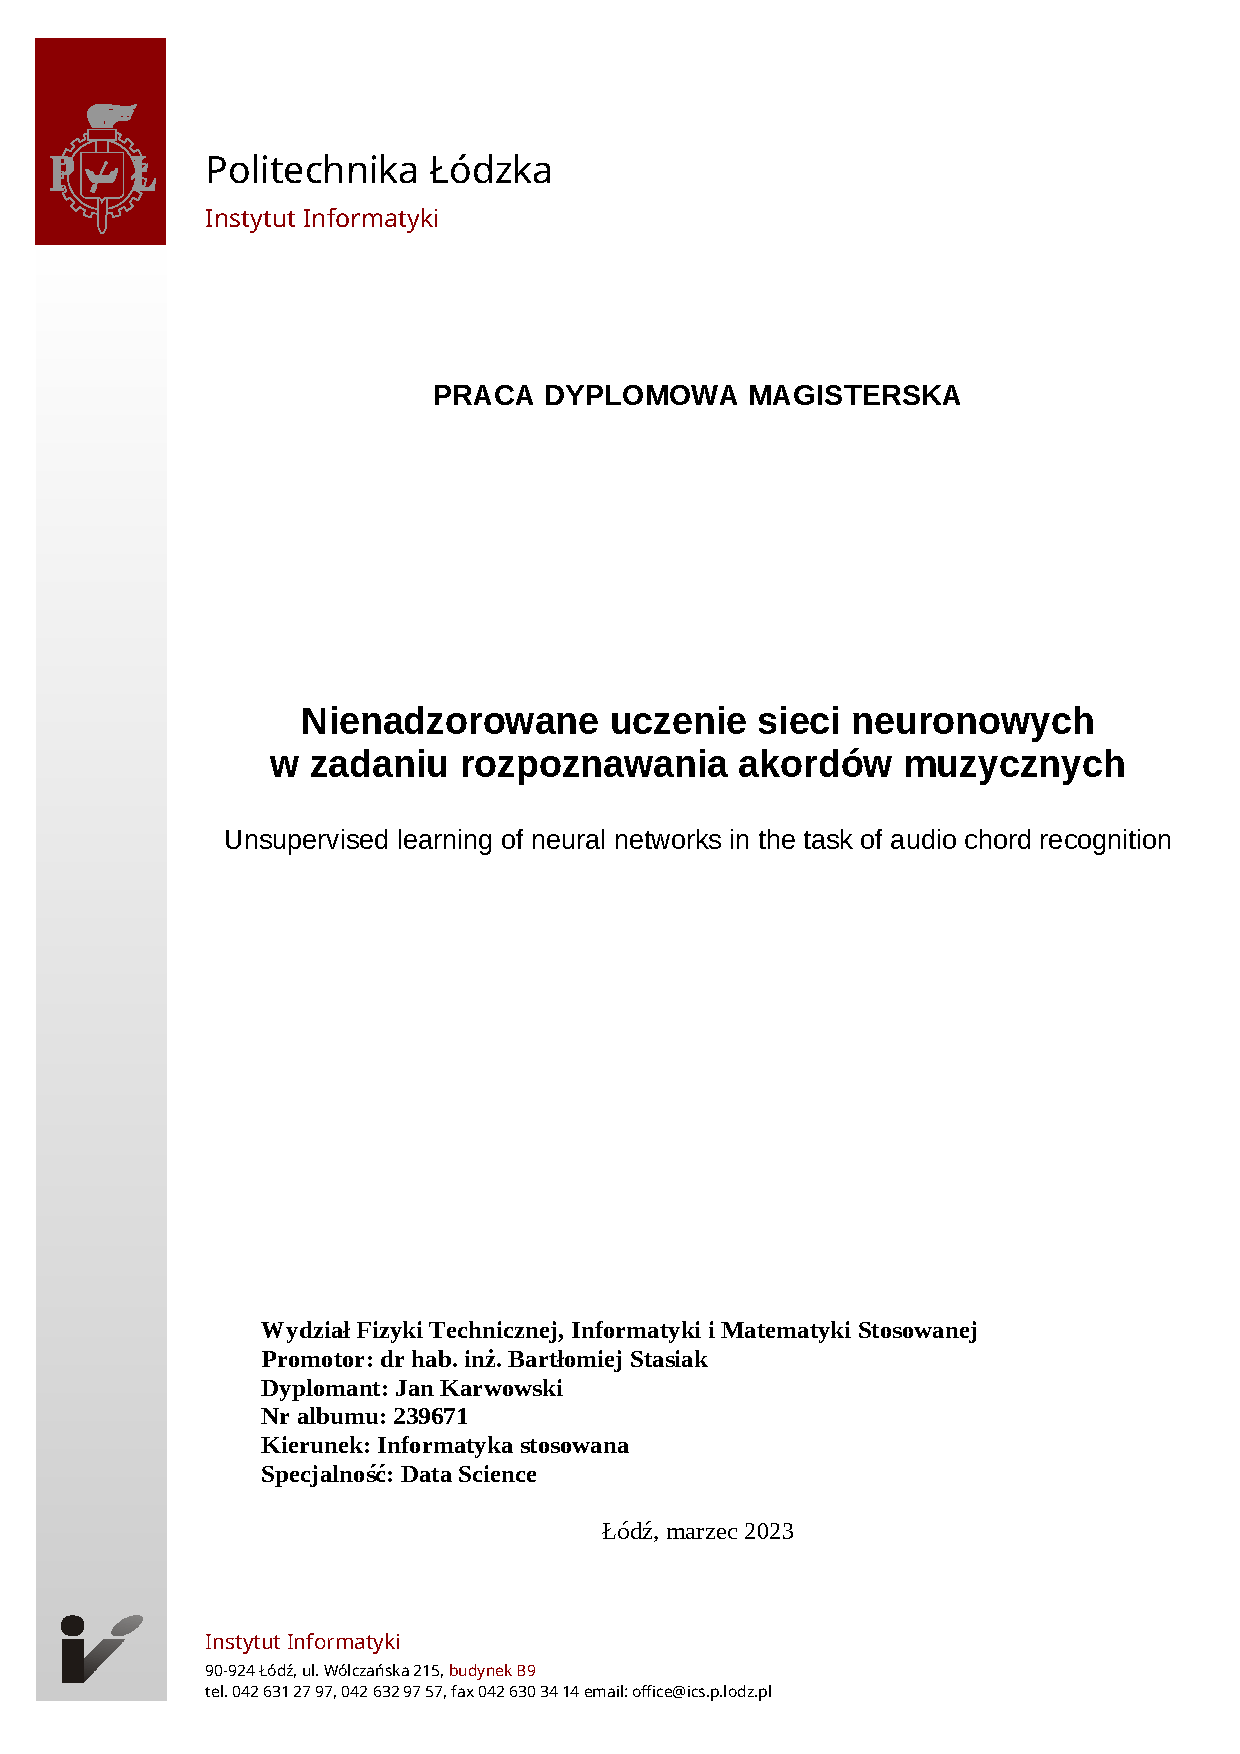
\includepdf{title_page}
\null\newpage

\tableofcontents

\chapter{Wstęp} \label{chapter:introduction}



\section{Problematyka i~zakres pracy}

% zakres
Niniejsza praca dotyczy zakresu cyfrowego przetwarzania sygnałów, sztucznej inteligencji i~uczenia maszynowego, a~w szczególności nadzorowanych i~nienadzorowanych sposobów uczenia głębokich sieci neuronowych.

% główny cel i~problematyka
Głównym celem pracy jest opracowanie i~przeanalizowanie algorytmu rozpoznawania akordów muzycznych bazującego na nienadzorowanych metodach uczenia sieci neuronowych. Na problematykę tę składają się więc dwa, dość luźno powiązane tematy:
\begin{itemize}
    \item automatyczne rozpoznawanie akordów muzycznych;
    \item nienadzorowane uczenie sieci neuronowych.
\end{itemize}

% ogólnie o~rozpoznawaniu akordów
Problem rozpoznawania akordów jest jednym z~podstawowych zadań z~dziedziny MIR (ang. \emph{Music Information Retrieval}) i~polega na automatycznym wyodrębnieniu z~nagrania muzycznego podstawowych struktur, jakimi są akordy --- różne układy brzmiących jednocześnie dźwięków. Automatyczne rozpoznawanie akordów może mieć wiele specjalistycznych zastosowań, takich jak ocenianie podobieństwa między utworami, rozpoznawanie gatunku czy automatyczne przygotowanie nut dla amatorów grania na gitarze. W~stosunku do innych zadań realizowanych za pomocą głębokich sieci neuronowych, takich jak klasyfikacja obrazów czy rozpoznawanie mowy, rozpoznawanie akordów jest stosunkowo proste. Istnieje już wiele dobrze sprawdzających się algorytmów realizujących to zadanie, zarówno starszych, bazujących na klasycznych metodach przetwarzania sygnałów, jak i~nowszych, opartych na uczeniu maszynowym, w~tym o~głębokie sieci neuronowe. 

% minusy rozpoznawania sieciami
Nowsze metody, bazujące głównie na sieciach neuronowych, wykazują się większą dokładnością niż klasyczne, deterministyczne algorytmy. Wymagają jednak uprzedniego przygotowania przez człowieka jak największej ilości poprawnych oznaczeń akordów dla wielu różnych utworów. Wymaga to dużo czasu i~specjalistycznej wiedzy oraz praktyki muzycznej. Ponadto oznaczenia takie pozostają mocno subiektywne i~trudno, aby były pozbawione błędów i~niedokładności.  Na podstawie gotowych przykładów sieć neuronowa uczy się sama realizować to zadanie. Dodatkowo proces nauki jest czasochłonny i~wymaga specjalistycznego sprzętu, jak karty graficzne, aby móc być zrealizowanym w~czasie nie dłuższym niż kilkanaście godzin. O~ile więc podejście to daje lepsze wyniki, jest znacznie trudniejsze w~realizacji i~narażone na wiele różnych błędów.

% wchodzi self-supervised
Częściowym rozwiązaniem powyższych problemów jest wykorzystanie nienadzorowanych metod uczenia sieci neuronowych. Metody te rozwijają się prężnie w~ostatnich latach i~pozwalają wykorzystać dane bez oznaczeń (np. losowe nagrania pobrane z~serwisów internetowych), aby nauczyć sieć neuronową struktury tychże danych i~występujących w~nich zależności. Przygotowane w~ten sposób modele sieci neuronowych mogą być później uczone realizacji konkretnych zadań metodami nadzorowanymi. Podejście to prowadzi do potencjalnych korzyści, takich jak:
\begin{itemize}
    \item krótszy czas nauki zadania docelowego (jeden model wytrenowany w~sposób nienadzorowany może być wykorzystany do wielu zadań docelowych);
    \item mniejsza ilość danych, wymaganych do nauki;
    \item lepsze generalizacja i~ogólnie lepsze wyniki.
\end{itemize}
Zadanie rozpoznawania akordów nadaje się więc idealnie, aby zastosować w~nim powyższe podejście. Pojawiły się już pierwsze próby stosowania metod nienadzorowanych w~zadaniu rozpoznawania akordów. Badania te są jednak jeszcze bardzo nieliczne i~niedojrzałe. Zdecydowanie pełen potencjał metod nienadzorowanych, który można obserwować w~popularniejszych dziedzinach jak przetwarzanie obrazu i~tekstu naturalnego, nie został jeszcze wykorzystany ani tutaj, ani w~całej dziedzinie MIR.

% wyzwania
Podejmując tematykę rozpoznawania akordów z~wykorzystaniem nienadzorowanych metod uczenia sieci neuronowych, trzeba zmierzyć się z~całym mnóstwem wyzwań. Po pierwsze i~najważniejsze, należy zgromadzić dwa zbiory danych. Pierwszym jest mniejszy zbiór danych oznaczonych, niezbędny, aby ostatecznie nauczyć sieć rozpoznawać akordy. Drugim jest najlepiej wielokrotnie większy zbiór danych bez oznaczeń, który będzie wykorzystany do treningów nienadzorowanych. Podczas gromadzenia danych trzeba zmierzyć się z~problemami ich jakości, zaszumienia błędnymi przykładami, odpowiednich rozkładów i~metod przechowywania. Po drugie, trzeba przygotować algorytm uczenia nienadzorowanego, który będzie adaptował istniejące już rozwiązania z~innych, większych i~lepiej finansowanych dziedzin, w~szczególności przetwarzania obrazów, rozpoznawania mowy i~przetwarzania języka naturalnego. Na końcu trzeba przeprowadzić serię czasochłonnych i~zasobożernych eksperymentów, których celem jest wykazać korzyści z~treningu nienadzorowanego. Korzyści te wcale nie muszą się wyraźnie pojawić i~należy zadbać o~ostrożną i~rozsądną interpretację wyników.

% wyniki
W~wyniku doświadczeń przeprowadzonych w~ramach niniejszej pracy, udało się wykazać korzyści z~treningu nienadzorowanego. Głównym znalezionym zyskiem jest wielokrotnie krótszy czas treningu i~nieznacznie poprawione wyniki. Przeprowadzone badania są jednak bardzo ograniczone i~absolutnie nie wyczerpują podjętego tematu pracy.



\section{Cele pracy}

\subsubsection{Zapoznanie się ze współczesnymi metodami nienadzorowanego uczenia sieci i~ich popularyzacja}

Pierwszym celem poznawczym pracy było zebranie informacji na temat metod uczenia sieci neuronowych bez nadzoru, czyli wykorzystując ogólnodostępne dane bez oznaczeń. Metody te rozwijają się w~ostatnich latach i~są wykorzystywane zwłaszcza w~dziedzinach takich jak rozpoznawanie obrazu, rozpoznawanie mowy i~analiza języka naturalnego. Stanowią ciekawy i~rozsądny kierunek rozwoju głębokich sieci neuronowych, umożliwiający osiąganie zupełnie nowych rezultatów.

\subsubsection{Zapoznanie się z~metodami rozpoznawania akordów muzycznych, bazującymi na sieciach neuronowych}

Drugim celem poznawczym było zebranie i~analiza literatury dotyczącej rozpoznawania akordów za pomocą sieci neuronowych. Przegląd ten miał służyć zorientowaniu się, na jakim etapie są badania nad tym konkretnym, jak i~również innymi problemami z~dziedziny MIR. Na tej podstawie można zaproponować wiele potencjalnych usprawnień i~kierunków rozwoju zaadoptowanych z~bardziej rozwiniętych obszarów jak przetwarzanie języka naturalnego.

\subsubsection{Zgromadzenie jak największych zbiorów danych oznaczonych i~nieoznaczonych oraz automatyzacja tego procesu}

Pierwszym praktycznym zadaniem realizowanym w~ramach niniejszej pracy jest zgromadzenie odpowiednio dużych zbiorów danych oznaczonych i~nieoznaczonych. Gromadzenie, organizacja i~wstępne przetwarzanie danych stanowi zawsze kluczowy element w~zadaniach rozwiązywanych za pomocą uczenia maszynowego. W~niniejszej pracy podjęta została próba jak największej automatyzacji tego czasochłonnego procesu, ocenione również zostały skutki zaproponowanego podejścia.

\subsubsection{Zaprojektowanie i~wykorzystanie algorytmu nienadzorowanego uczenia sieci neuronowych w~zadaniu rozpoznawania akordów muzycznych}

W~ramach niniejszej pracy powstała propozycja algorytmu uczenia nienadzorowanego, który może być wykorzystany i~przynieść korzyści w~realizacji zadania rozpoznawania akordów muzycznych. Algorytm ten jest bardzo prosty i~stanowi jedynie adaptację pewnego podejścia, wykorzystywanego w~obszarach przetwarzaniu języka naturalnego, analizy obrazu i~rozpoznawania mowy.

\subsubsection{Zbadanie korzyści z~zaproponowanego rozwiązanie poprzez przeprowadzenie odpowiednich eksperymentów}

Zaproponowane rozwiązanie zostało w~miarę możliwości zbadane empirycznie, poprzez przeprowadzenie odpowiednich eksperymentów. Wykonane zostały więc serie różnych treningów różnych modeli sieci neuronowych, mających na celu ocenić korzyści z~zaproponowanego podejścia. Wszystkie eksperymenty zostały dokładnie udokumentowane i~szczegółowo opisane.



\section{Metoda badawcza}

W~pierwszej kolejności przeanalizowana została cała znaleziona literatura, dotycząca rozpoznawania akordów za pomocą sieci neuronowych. Są to głównie pochodzące z~wielu różnych źródeł i~zagregowane na platformach internetowych artykuły naukowe, dostępne w~języku angielskim. Taką samą formę mają również prace stanowiące drugą część przeglądu, czyli odnoszące się do nienadzorowanego uczenia sieci neuronowych. Ze względu na ich ogromną ilość, przejrzana i~opisana została jedynie mała część, co istotniejszych prac na ten temat. Związane są one z~bardzo różnymi obszarami, takimi jak przetwarzanie tekstu naturalnego, analiza obrazu, rozpoznawanie mowy, rozpoznawanie innych dźwięków, a~nawet pierwsze podejścia do wykorzystania nienadzorowanego uczenia w~rozpoznawaniu akordów.

Drugim etapem pracy była adaptacja istniejących metod uczenia nienadzorowanego do dziedziny przetwarzania utworów muzycznych. Wybrane zostało w~szczególności jedno podejście do nienadzorowanego treningu sieci neuronowych i~wykorzystane przy projektowaniu ostatecznej formy zaproponowanego w~ramach niniejszej pracy algorytmu.

Skuteczność zaproponowanego algorytmu została oceniona poprzez odpowiednie eksperymenty, których głównym celem było wykazanie korzyści z~zaproponowanego podejścia. Wybrana została więc jedna praca \cite{park_bi-directional_2019}, prezentująca ostatnie, najlepsze wyniki na zadaniu rozpoznawania akordów. Podejście autorów, sprowadzające się do odpowiedniej procedury wstępnego przetwarzania danych i~odpowiedniej architektury modelu sieci neuronowej, zostało zreprodukowane i~nieznacznie uproszczone. W~ten sposób przygotowane zostało środowisko do przeprowadzenia eksperymentów. Następnie, przeprowadzone zostały dwa treningi nienadzorowane i~seria treningów nadzorowanych, podczas których wykazana została przydatność i~skuteczność treningów nienadzorowanych.



\section{Przegląd literatury w~dziedzinie}

Przegląd literatury jak wspomniano wcześniej, składa się z~dwóch głównych części. Pierwsza część dotyczy rozpoznawania akordów, ale tylko z~wykorzystaniem sieci neuronowych. Aby ograniczyć liczbę analizowanych prac, zrezygnowano z~tych, które dotyczą starszych metod, stosowanych przed rozpowszechnieniem się sieci neuronowych (z drobnymi wyjątkami). Skupiono się natomiast możliwie dokładnie na analizie rozwiązań opartych na sieciach neuronowych. Wyszukano w~tym celu i~zgromadzono niemalże wszystkie (zdaniem autora) opublikowane prace, gdzie próbowano rozpoznawać akordy modelami sieci neuronowych. Druga część przeglądu jest luźniejsza i~mniej szczegółowa, ponieważ dotyczy znacznie szerszego obszaru, jakim jest nienadzorowane uczenie sieci neuronowych. Stosowane jest ono w~bardzo różnych dziedzinach. Wyszukane zostały co ważniejsze i~bardziej interesujące w~kontekście rozpoznawania akordów prace, gdzie proponowano, analizowano i~adaptowano algorytmy nienadzorowanego uczenia sieci neuronowych. Algorytmy te dzielą się właściwie na dwie, powiązane ze sobą grupy: metody samonadzorowane (ang. \emph{self-supervised}) i~metody półnadzorowane (ang. \emph{semi-supervised}). Wszystkie te algorytmy mają natomiast ten sam cel: wykorzystać dane bez oznaczeń, aby później uzyskać lepsze wyniki na konkretnym zadaniu.

\subsection{Rozpoznawanie akordów za pomocą sieci neuronowych}

% początek (humphrey)
Pierwszą próbę rozpoznawania akordów muzycznych za pomocą sieci neuronowych podjęli Eric J. Humphrey i~Juan P. Bello w~2012 roku \cite{humphrey_rethinking_2012}. Opisali oni jak za pomocą splotowej sieci neuronowej, stosowanej wcześniej głównie w~rozpoznawaniu obrazów, można rozpoznawać akordy muzyczne. Ich pomysł zapoczątkował całą serię badań innych naukowców zajmujących się problemem ACR (ang. \emph{Audio Chord Recognition}), stanowiącym jedno z~podstawowych zadań z~dziedziny MIR (ang. \emph{Music Information Retrieval}). Zaproponowane przez nich rozwiązanie jest stosunkowo proste, dzisiaj natomiast już zdecydowanie wymagające usprawnień. Wynika to z~faktu, że faktyczny rozwój uczenia głębokiego (ang. \emph{deep learning}) rozpoczął się właśnie w~roku 2012 i~od tego czasu powstało całe mnóstwo metod pozwalających osiągnąć dokładniejsze wyniki mniejszym kosztem obliczeniowym.

% opis prac Korzeniowskiego
Jedną z~najobszerniejszych serii prac dotyczących rozpoznawania akordów muzycznych z~wykorzystaniem sieci neuronowych wykonali Korzeniowski i~Widmer \cite{korzeniowski_feature_2016,korzeniowski_fully_2016,korzeniowski_futility_2017,korzeniowski_improved_2018,korzeniowski_automatic_2018,korzeniowski_large-scale_2018}. W~ciągu kilku lat przeprowadzili szereg badań i~wydali sześć artykułów związanych z~tym tematem. Artykuły te wynikają kolejno jedne z~drugich i~nawzajem się uzupełniają. W~pierwszym z~nich \cite{korzeniowski_feature_2016} autorzy proponują użycie perceptronu wielowarstwowego do ekstrakcji cech dźwięku (ang. \emph{chroma feature}) w~miejsce wcześniej stosowanych deterministycznych, znacznie mniej skomplikowanych algorytmów ekstrakcji cech. Tak powstała reprezentacja jest ich zdaniem znacznie lepsza i~może zostać wykorzystana do dalszej klasyfikacji akordów, lub w~zupełnie innym celu. Dodatkowo pomysł ten jest motywowany założeniem, że to właśnie ekstrakcja cech z~surowych danych gra kluczową rolę w~jakości klasyfikacji akordów --- jest znacznie ważniejsza od późniejszego rozpoznawania konkretnego akordu i~detekcji całej sekwencji. W~kolejnej pracy \cite{korzeniowski_fully_2016} autorzy wykorzystują tym razem splotową sieć neuronową w~połączeniu z~CRF (ang. \emph{Conditional Random Fields}) aby stworzyć kompletny algorytm rozpoznający akordy. Daje on bardzo konkurencyjne wyniki, które do dziś praktycznie nie zostały znacząco poprawione. Rozwiązania te stanowią punkt odniesienia dla wielu kolejnych prac innych badaczy \cite{ohanlon_fifthnet_2021, park_bi-directional_2019}.

W~dalszym toku badań autorzy skupiają się na możliwości usprawnienia wcześniejszych rozwiązań poprzez wykorzystanie modeli językowych i~powiązania między zadaniem detekcji sekwencji akordów a~zadaniem detekcji i~zrozumienia sekwencji słów w~języku naturalnym. Najpierw udowadniają, że złożone modele językowe (sieci rekurencyjne) nie sprawdzą się dobrze, jeśli będą stosowane na poziomie pojedynczych ramek czasowych, a~nie pojedynczych wystąpień akordów \cite{korzeniowski_futility_2017}. W~takiej sytuacji lepiej sprawdzają się znacznie prostsze modele jak HMM (ang. \emph{Hidden Markov Model}), które w~praktyce jedynie ,,wygładzają'' sekwencję akordów. W~kolejnych badaniach \cite{korzeniowski_large-scale_2018} wykazują, że modele stosowane do przetwarzania języka naturalnego (ang. \emph{Natural Language Processing}) mają duży potencjał i~potrafią skutecznie modelować zależności w~sekwencjach akordów muzycznych (np. przewidywać cykle), co pozwala usprawnić ogólną jakość klasyfikacji akordów. Autorzy opisują w~końcu model probabilistyczny, pozwalający połączyć model akustyczny (rozpoznający akordy w~danej chwili czasu) z~modelem językowym (dekodującym całą sekwencję pojedynczych akordów), implementują go i~przeprowadzają szereg eksperymentów pozwalających potwierdzić, że tak zastosowane złożone modele językowe usprawniają jakość klasyfikacji akordów \cite{korzeniowski_improved_2018}.

O~ile opisane powyżej prace stanowią bardzo istotny wkład w~dziedzinę badań nad zadaniem ACR i~porządkują wiele aspektów tego zagadnienia (jak kwestia wykorzystania modeli językowych), to w~obecnej chwili są już raczej przestarzałe. Spostrzeżenia i~wnioski zawarte w~tych pracach pozostają w~większości aktualne, jednakże nie ma sensu stosowanie wykorzystywanych wtedy architektur sieci neuronowych, ze względu na możliwość wykorzystania nowszych modeli, dokładniejszych i~wydajniejszych obliczeniowo.

% structured training (o niezbalansowaniu)
Równolegle do prac Korzeniowskiego i~Widmera, jak również już po ich ostatnich publikacjach związanych z~tym tematem, powstawało wiele innych prac dotyczących zadania rozpoznawania akordów muzycznych za pomocą sieci neuronowych. Wśród nich warto wspomnieć \cite{mcfee_structured_2017}, gdzie autorzy próbują rozwiązać problem niezbalansowanych zbiorów danych (w praktyce niektóre akordy występują znacznie rzadziej niż inne, a~do tego są bardzo podobne do tych występujących częściej) poprzez ,,ustrukturyzowanie'' treningu. Rozwiązanie to w~uproszczeniu polega na dołożeniu dodatkowych funkcji kosztu dla sieci neuronowej (dodatkowego nadzorowania), wymuszających ekstrakcję pewnych konkretnych (wspólnych między akordami) cech. Wszystko to pozwala osiągnąć trochę lepsze wyniki, jednakże wadą jest skomplikowanie rozwiązania. Ponadto sama idea i~kierunek badań mogą zostać poddane w~wątpliwość, ze względu na dużą ingerencję w~sposób działania sieci neuronowej i~wymuszanie pewnych zachowań. Alternatywą jest dążenie w~kierunku generalizacji i~faktycznego polegania na danych uczących, a~nie na wiedzy dziedzinowej (tzw. podejście \emph{data driven}). Przykładem takiego kierunku badań są właśnie metody nienadzorowanego uczenia sieci neuronowych.

% użycie transformerów
W~przetwarzaniu języka naturalnego już od kilku lat standardem jest architektura zwana Transformerem \cite{vaswani_attention_2017}, która pozwala zrównoleglić obliczenia wcześniej przeprowadzane sekwencyjne i~w ogóle pozwala osiągnąć wyniki lepsze, niż stosowane wcześniej do tego zadania sieci rekurencyjne. Niedawno architektura ta weszła również do użytku w~przetwarzaniu obrazów \cite{dosovitskiy_image_2021} i~obecnie modele tego typu osiągają wyniki lepsze niż klasyczne splotowe sieci neuronowe. Jeszcze przed wprowadzeniem Transformerów do przetwarzania obrazów wykonane zostały co najmniej dwie próby wykorzystania tej architektury do zadania rozpoznawania akordów. Pierwsza z~nich \cite{chen_harmony_2019} jest trudna do oceny ze względu na małą liczbę przeprowadzonych eksperymentów oraz brak realnego odniesienia do rozwiązań innych autorów. Natomiast w \cite{park_bi-directional_2019} pokazane zostało, że Transformer może dać wyniki bardzo zbliżone do osiąganych w \cite{korzeniowski_fully_2016}. Chociaż transformer nie pozwolił osiągnąć lepszych wyników, to należy pamiętać, że była to zaledwie pierwsza próba wykorzystania tej architektury, która w~najprostszej postaci sprawdziła się zupełnie zadowalająco. Można dodać, że po wprowadzeniu transformerów do przetwarzania obrazów, zostały one również w~podobny sposób wykorzystane do klasyfikacji dźwięków \cite{gong_ast_2021}.

% fifthnet
Warto jeszcze wspomnieć o~dwóch bardzo istotnych pracach, jakimi są \cite{hanlon_fifthnet_2020} oraz \cite{ohanlon_fifthnet_2021}. Pomysł autorów polega tam na radykalnym zmniejszeniu liczby parametrów sieci, na rzecz specjalistycznej architektury, odpowiedniej do problemu rozpoznawania akordów. Udało się wykazać tam, że wielokrotnie mniejszy model jest w~stanie osiągnąć tak samo dobre wyniki, jak \cite{korzeniowski_fully_2016}, przy odpowiednim formacie danych wejściowych i~odpowiednim układzie warstw sieci neuronowej. Prace te są o tyle ważne, że pokazują, iż problem rozpoznawania akordów nie jest bardzo złożony, zwłaszcza w~porównaniu z~takimi zadaniami, jak klasyfikacja obrazów czy rozpoznawanie mowy.

\subsection{Nienadzorowane uczenie sieci neuronowych}

% chaotycznie o~uczeniu nienadzorowanym
Choć próby realizacji uczenia sieci neuronowych bez oznaczeń były stosowane już wcześniej \cite{noroozi_unsupervised_2017}, to stały się tak naprawdę przydatne w~momencie, kiedy wykorzystano je w~przetwarzaniu języka naturalnego \cite{devlin_bert_2019}. W~tym obszarze stosowanie treningów nienadzorowanych, a~dokładnie samonadzorowanych, stało się właściwie standardem. Jeżeli chodzi o~obszar przetwarzania obrazów, to tutaj sytuacja ma się nieco inaczej. Wcześniejsze próby, takie jak \cite{pathak_context_2016}, czy \cite{noroozi_unsupervised_2017} nie przyniosły szczególnych rezultatów. Wciąż bardziej opłacało się trenować na dużych zbiorach do klasyfikacji i~ewentualnie dotrenowywać na zadaniu docelowym. Sytuacja ta wynika również ze znacznie większej niż w~przypadku analizy tekstu naturalnego, dostępności danych oznaczonych. Jednakże z~czasem, coraz więcej nowych pomysłów zaczęło się pojawiać i~powstały między innymi takie serie prac jak \cite{chen_simple_2020, grill_bootstrap_2020, caron_unsupervised_2021, caron_emerging_2021}, które dotyczą stricte samonadzorowanego uczenia na obrazach poprzez sprytne wykorzystanie augmentacji. Metody te nie rozpowszechniły się tak bardzo, jak w~innych obszarach, być może również ze względu na swoją złożoność. Nie wydają się one również tak dobrze pasować do zadania rozpoznawania akordów, które jednak znacznie bardziej zbliżone jest do przetwarzania tekstu, a~najbardziej do innych form analizy dźwięku, np. rozpoznawania mowy. To właśnie w~tym ostatnim obszarze, podobnie jak w~przetwarzaniu języka naturalnego, bardzo powszechnym stało się korzystanie z~metod samonadzorowanych, takich jak \cite{baevski_wav2vec_2020}. Innymi przykładami stosowania metod samonadzorowanych w~analizie dźwięku są dwie bardzo podobne prace \cite{baade_mae-ast_2022} i \cite{he_masked_2021}. Obie bazują na kluczowym dla niniejszej pracy pomyśle o~nazwie MAE \cite{he_masked_2021}, który pochodzi akurat z~dziedziny przetwarzania obrazów, ale tak naprawdę jest jedynie udaną adaptacją, pochodzącego z~przetwarzania języka naturalnego, słynnego \cite{devlin_bert_2019}.

% bardziej o~semi-supervised
Po części alternatywnym pomysłem do treningów samonadzorowanych są treningi półnadzorowane. Warto wspomnieć o~dwóch bardzo udanych pracach, jakimi są związane z~przetwarzaniem obrazów \cite{xie_self-training_2020} oraz \cite{pham_meta_2021}. W~przeciwieństwie do metod samonadzorowanych algorytmy te okazały się bardzo praktyczne i~zostały wykorzystane przy osiąganiu najwyższych wyników w~szeroko rozumianej klasyfikacji obrazów. Co ciekawe, jeżeli chodzi o~metody nienadzorowane w~rozpoznawaniu akordów, to również należą one bardziej do grupy półnadzorowanych. Powstały zwłaszcza dwie takie prace. Pierwszą jest \cite{wu_semi-supervised_2020}, w~której autorzy wykorzystują autoenkoder wariacyjny. Jeżeli chodzi o~uzyskaną poprawę, to zaznaczają oni, że wykorzystanie zaproponowanego przez nich algorytmu poprawia jakość klasyfikacji w~stosunku do prostego uczenia nadzorowanego na tych samych danych. Niestety nie porównują się do innych algorytmów. Pokazują natomiast wpływ proporcji danych oznaczonych i~nieoznaczonych na otrzymaną dokładność. Drugim algorytmem jest \cite{bortolozzo_improving_2021}, w~którym autorzy zaadaptowali wspomniany wcześniej \cite{xie_self-training_2020} do zadania rozpoznawania akordów. Jeżeli chodzi o~uzyskaną poprawność, to wyniki prezentowane w~tej pracy są całkiem spektakularne --- wielokrotnie poprawia się dokładność klasyfikacji rzadko występujących akordów.



\section{Układ pracy}

Tematem pracy jest: ,,Nienadzorowane uczenie sieci neuronowych w~zadaniu rozpoznawania akordów muzycznych'', za główny zaś cel przyjęto zaproponowanie i~przetestowanie algorytmu nienadzorowanego uczenia sieci neuronowych w~zadaniu rozpoznawania akordów. Rozdział \ref{chapter:introduction} zawiera wstęp i~cele pracy oraz przegląd literatury. Rozdział \ref{chapter:music_theory} wprowadza niezbędny zestaw pojęć z~obszaru cyfrowego przetwarzania sygnałów i~teorii muzyki oraz wyjaśnia, czym właściwie są akordy. W~rozdziale \ref{chapter:dataset} szczegółowo przedstawiony został proces gromadzenia i~wstępnego przetwarzania zbiorów danych. Następnie w~rozdziale \ref{chapter:methodology} opisany został dokładnie zaproponowany algorytm oraz wprowadzone zostały niezbędne pojęcia z~dziedziny uczenia maszynowego i~sieci neuronowych. Rozdział \ref{chapter:experiments} prezentuje szczegółowy opis przeprowadzonych eksperymentów oraz wyniki i~ich dyskusję. W~podsumowaniu pracy przedstawiono najważniejsze obserwacje i~wnioski z~przeprowadzonych eksperymentów, z~których wynika, że metody nienadzorowane są przydatne i~mają potencjał, aby być stosowane w~zadaniu rozpoznawania akordów i~innych zadaniach z~dziedziny MIR. Wnioski te stanowią najważniejszy rezultat niniejszej pracy.

\chapter{Sygnał dźwiękowy i podstawy teorii muzyki} \label{chapter:music_theory}

Niniejszy rozdział zawiera wprowadzenie teoretyczne, niezbędne do zrozumienia koncepcji akordu i wykorzystanych algorytmów wstępnego przetwarzania utworów muzycznych. Po pierwsze przedstawione zostały absolutne podstawy z obszaru cyfrowego przetwarzania sygnałów, czyli DSP (ang. \emph{Digital Signal Processing}), ponieważ przetwarzanie dźwięku za pomocą komputera stanowi właśnie formę cyfrowego przetwarzania sygnału. Dalej wprowadzony został szereg pojęć z teorii muzyki, zmierzający do wyjaśnienia czym właściwie jest akord muzyczny. Na końcu dodany został krótki opis nieskomplikowanego, historycznego już, najbardziej podstawowego algorytmu automatycznego rozpoznawania akordów muzycznych.



\section{Podstawy cyfrowego przetwarzania sygnałów}

Sygnał dźwiękowy może być opisany jako zmiany poziomu ciśnienia akustycznego w funkcji czasu\footnote{\cite{lerch_introduction_2012}, s. 7}. W praktyce oznacza to okresowe drganie cząsteczek powietrza lub innego ośrodka, które rozchodzi się w postaci fali (dźwiękowej) i może zostać zarejestrowane przez narząd słuchu. Aby było to możliwe, parametry sygnału dźwiękowego muszą mieścić się w określonym zakresie. Różne stworzenia posiadają różne granice słyszalności i tak np. pies jest w stanie usłyszeć dźwięki, których człowiek nie potrafi w żaden sposób zauważyć. 

Będący tematem tego rozdziału sygnał dźwiękowy (określany również po prostu jako \emph{dźwięk}) posiada wiele parametrów i może podlegać najróżniejszym analizom i przekształceniom.  Oczywiście sygnał dźwiękowy może pochodzić z różnych źródeł i analizowanie tego sygnału może mieć wszelakie cele, od rozpoznawania zbliżającej się straży pożarnej, poprzez rozpoznawanie mowy, aż do analizy utworu muzycznego i konkretnych jego cech. Z punktu widzenia niniejszej pracy to właśnie ten ostatni przypadek jest istotny i wszelkie operacje przetwarzania sygnału będą dokonywane na fragmentach utworów muzycznych.

% sygnał cyfrowy - próbkowanie i kwantyzacja
Ponieważ tworzony w ramach tej pracy system działa w środowisku cyfrowym, niemożliwa jest tam idealnie zgodna z rzeczywistością reprezentacja sygnału dźwiękowego. W praktyce wykorzystywana do przetwarzania jest jego cyfrowa reprezentacja, która ma formę dyskretną zarówno co do czasu, jak i co do amplitudy. Zatem przed właściwym przystąpieniem do przetwarzania sygnału dźwiękowego, podczas procesu rejestracji za pomocą dedykowanego urządzenia --- mikrofonu, który zamienia zmiany ciśnienia akustycznego na zmiany napięcia, sygnał ulega dwóm przekształceniom, przedstawionym na rys.  \ref{fig:probkowanie_i_kwantyzacja}. Pierwsze to \emph{próbkowanie}\footnote{\cite{lerch_introduction_2012}, s. 9} z pewną częstotliwością $f_p$, polegające na tym, że czas ulega dyskretyzacji i z ciągłego sygnału dźwiękowego zapisane są jedynie niektóre wartości, równomiernie oddalone od siebie o $T_s=1/f_p$ sekundy. Po drugie \emph{kwantyzacja}\footnote{\cite{lerch_introduction_2012}, s. 11}, czyli zaokrąglenie wartości amplitudy do najbliższej z wcześniej zdefiniowanego zbioru $N$ możliwych wartości. Liczba dozwolonych wartości amplitudy determinuje liczbę $w$ bitów pamięci komputera potrzebnych na zapisanie pojedynczej próbki sygnału, zgodnie ze wzorem $w=\log_{2}N$.

\begin{figure}[htb]
    \centering
    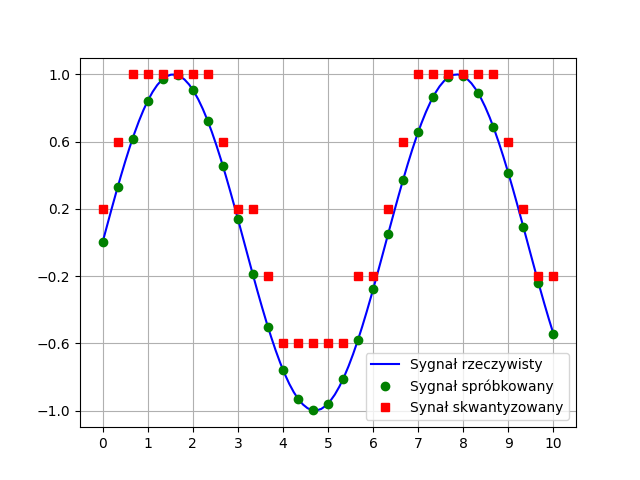
\includegraphics[width=0.9\textwidth]{images/probkowanie_i_kwantyzacja}
    \caption{Operacje próbkowania i kwantyzacji.}
    \label{fig:probkowanie_i_kwantyzacja}
\end{figure}

% sygnał okresowy i losowy
Sygnał dźwiękowy może być \emph{sygnałem okresowym} lub \emph{sygnałem losowym}\footnote{\cite{lerch_introduction_2012}, s. 7-8}. Pierwszy z nich powtarza się co określony odcinek czasu $T_0$, a drugi nie jest przewidywalny i jego wartości są zupełnie losowe. Przykładem pierwszego z nich jest dźwięk pianina, przedstawiony na rys \ref{fig:sygnal_okresowy}, gdzie da się dostrzec widoczną powtarzalność pewnego odcinka sygnału.  Sygnał losowy w postaci tzw. białego szumu został przedstawiony na rys. \ref{fig:sygnal_losowy}.

\begin{figure}[htb]
    \centering
    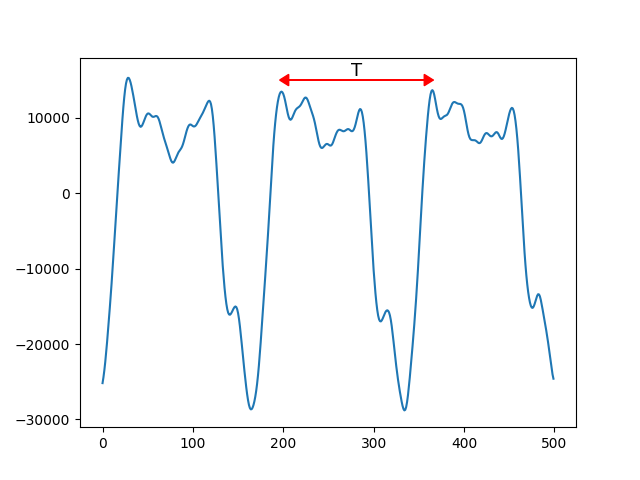
\includegraphics[width=0.9\textwidth]{images/sygnal_okresowy}
    \caption{Przykładowy sygnał okresowy - pojedynczy dźwięk pianina.}
    \label{fig:sygnal_okresowy}
\end{figure}

\begin{figure}[htb]
    \centering
    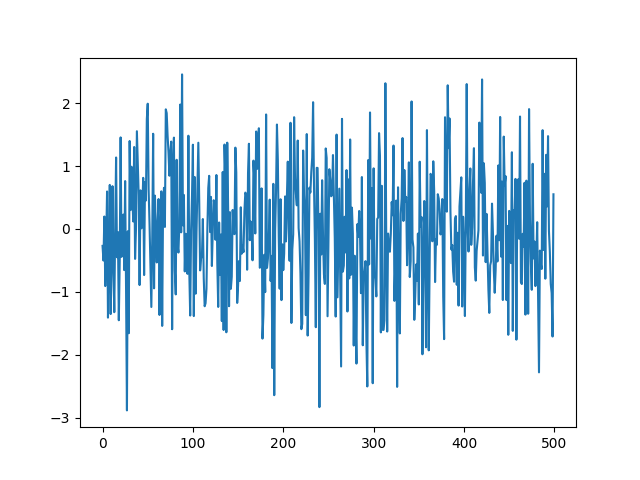
\includegraphics[width=0.9\textwidth]{images/sygnal_losowy}
    \caption{Przykładowy sygnał losowy - biały szum.}
    \label{fig:sygnal_losowy}
\end{figure}

% częstotliwości składowe
Sygnał losowy jest mniej istotny z punktu widzenia tej pracy. Ma on swoje miejsce w muzyce i niektóre instrumenty (zwłaszcza perkusyjne) mogą być jego źródłem. Jednakże, aby dało się we fragmencie sygnału dźwiękowego wyróżnić akord, musi to być sygnał okresowy. Na rys. \ref{fig:probkowanie_i_kwantyzacja} oryginalny sygnał jest \emph{tonem prostym}. Oznacza to, że zawiera on w sobie tylko jedną \emph{częstotliwość składową}, którą da się tam wyraźnie zauważyć. W przyrodzie właściwie nie występują tony proste. Różne odgłosy przyrody ożywionej i nieożywionej, dźwięki instrumentów czy ludzki głos zawsze posiadają więcej częstotliwości składowych, tworzących dany sygnał. Widać to na rys. \ref{fig:sygnal_okresowy}, gdzie przedstawiono fragment sygnału dźwiękowego pochodzącego z pianina. Da się tutaj gołym okiem zauważyć najniższą częstotliwość składową, tzw. \emph{częstotliwość podstawową} (odpowiadający jej okres jest zaznaczony czerwoną strzałką). Nie jest to jednak jedyna częstotliwość obecna w tym sygnale i fakt, że wykres ten jest tak ,,pofalowany'' to właśnie skutek obecności innych, wyższych składowych. Składowe te decydują o barwie i charakterze dźwięku, sprawiają, że jesteśmy w stanie rozróżnić instrumenty i ludzi, chociażby wydawali z siebie dźwięk o tej samej częstotliwości podstawowej. 

% DFT
Podstawowym narzędziem pozwalającym wyróżnić częstotliwości składowe sygnału jest \emph{Transformacja Fouriera}\footnote{\cite{lyons_wprowadzenie_2000}, s. 61}. Oryginalnie jest ona zdefiniowana dla sygnału ciągłego, ale istnieje również jej dyskretna wersja, w skrócie DFT (ang. \emph{Discrete Fourier Transform}).  Przekształca ona sygnał $x$ o długości $N$ w sygnał $X$ o tej samej długości, zgodnie ze wzorem:
\begin{equation} \label{eq:dft}
    X(k) = \sum_{n=1}^{N} x(n) e^{-ink \frac{2 \pi}{N}}
\end{equation}
gdzie $k$ to numer próbki sygnału wyjściowego $X$ (odpowiadającej pojedynczej częstotliwości), $n$ to numer próbki sygnału wejściowego $x$, a $i$ to jednostka urojona.

% STFT
Czasami stosuje się również pojęcie STFT (ang. \emph{Short Time Fourier Transform})\footnote{\cite{lerch_introduction_2012}, s. 20}, które właściwie oznacza to samo co DFT, tylko odnosi się do dłuższego fragmentu sygnału, który dzieli się na bloki i dopiero dla każdego z nich wykonuje się DFT. Wynik STFT jest więc macierzą, gdzie każdy wiersz zawiera wynik DFT dla pojedynczego bloku (ramki) sygnału. Jeżeli sygnał jest próbkowany z częstotliwością $f_s$, to wtedy wartość $k$ sygnału wynikowego $X$ informuje o fazie i natężeniu składowej o częstotliwości $f(k) = \frac{f_s}{N}k$.  Oczywiście, jak widać we wzorze \ref{eq:dft}, wynik transformacji Fouriera ma postać zespoloną. Aby uzyskać natężenie danej składowej należy wziąć wartość bezwzględną liczby zespolonej, jej argument informuje natomiast o przesunięciu fazowym danej składowej. Na rys.  \ref{fig:transformata_fouriera} przedstawiono wynik przeprowadzenia opisanych powyżej operacji na dwóch przykładowych sygnałach --- tonie prostym o jednej częstotliwości składowej i bardziej złożonym sygnale, będącym złożeniem trzech częstotliwości. Warto jeszcze zaznaczyć, że jeżeli sygnał wejściowy ma wartości rzeczywiste, to wynik DFT jest symetryczny\footnote{\cite{lyons_wprowadzenie_2000}, s. 72} i dlatego uwzględnia się tylko jego pierwszą połowę.

\begin{figure}[htb]
    \centering
    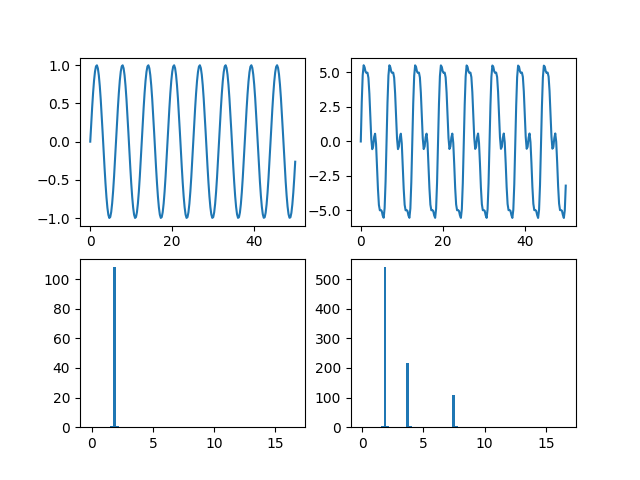
\includegraphics[width=0.9\textwidth]{images/transformata_fouriera}
    \caption{Wyniki Transformacji Fouriera (dolny rząd) dla dwóch przykładowych sygnałów (górny rząd).}
    \label{fig:transformata_fouriera}
\end{figure}

% FFT
W praktyce nie wylicza się DFT bezpośrednio ze wzoru, ponieważ wiąże się to z kwadratową złożonością obliczeniową, co zupełnie uniemożliwia przetwarzanie w czasie rzeczywistym. Korzysta się z szybkiej wersji algorytmu o nazwie FFT (ang. \emph{Fast Fourier Transform})\footnote{\cite{lyons_wprowadzenie_2000}, s. 132}, którego omówienie wykracza poza zakres tej pracy.

% funkcje okna
Jeżeli składowe sygnału poddawanego transformacji Fouriera nie pokrywają się idealnie z częstotliwościami odpowiadającymi poszczególnym punktom transformaty, dochodzi do \emph{przecieku}\footnote{\cite{lyons_wprowadzenie_2000}, s. 80}. Polega on na tym, że energia takiej składowej uwidacznia się we wszystkich wartościach wyniku DFT. Aby minimalizować to zjawisko, stosuje się \emph{funkcje okna}. Jest to funkcja, którą stosuje się dla fragmentu sygnału o długości $N$ próbek, przed przeprowadzeniem na nim DFT. Przykładową funkcją okna jest \emph{okno Hanninga}, które wyraża się wzorem:
\begin{equation}
    f(n) = 0.5 - 0.5 \cos (2 \pi n / N)
\end{equation}
gdzie $n$ jest numerem próbki sygnału a $N$ liczbą próbek.

% spektrogramy
Do przeprowadzenia analizy \emph{widma} (czyli częstotliwości składowych) fragmentu pewnego sygnału, DFT nadaje się idealnie. Jednakże utwory muzyczne w muzyce popularnej trwają zazwyczaj kilka minut i podczas ich analizy bardzo ważne jest, aby uwzględnić zmiany dźwięków w czasie. Sam wynik DFT nie niesie żadnej informacji o zmianach częstotliwości składowych, jedynie o ich obecności, fazie i natężeniu.  W praktyce reprezentuje się więc sygnał dźwiękowy w postaci \emph{spektrogramu}\footnote{\cite{lerch_introduction_2012}, s. 21}, który jest dwuwymiarową reprezentacją dźwięku i zawiera informację o natężeniu częstotliwości składowych sygnału w kolejnych chwilach czasu. Aby utworzyć taki spektrogram, którego przykład został zaprezentowany na rys.  \ref{fig:spektrogram}, należy podzielić sygnał na niewielkie, trwające np. ułamek sekundy części. Na każdej z nich przeprowadza się DFT, wylicza moduł wartości zespolonych i ostatecznie otrzymuje się natężenie częstotliwości składowych dla każdego z wydzielonych kawałków. Właściwie jest to więc wspomniana wcześniej operacja STFT, która jest jednym ze sposobów tworzenia spektrogramu.

\begin{figure}[htb]
    \centering
    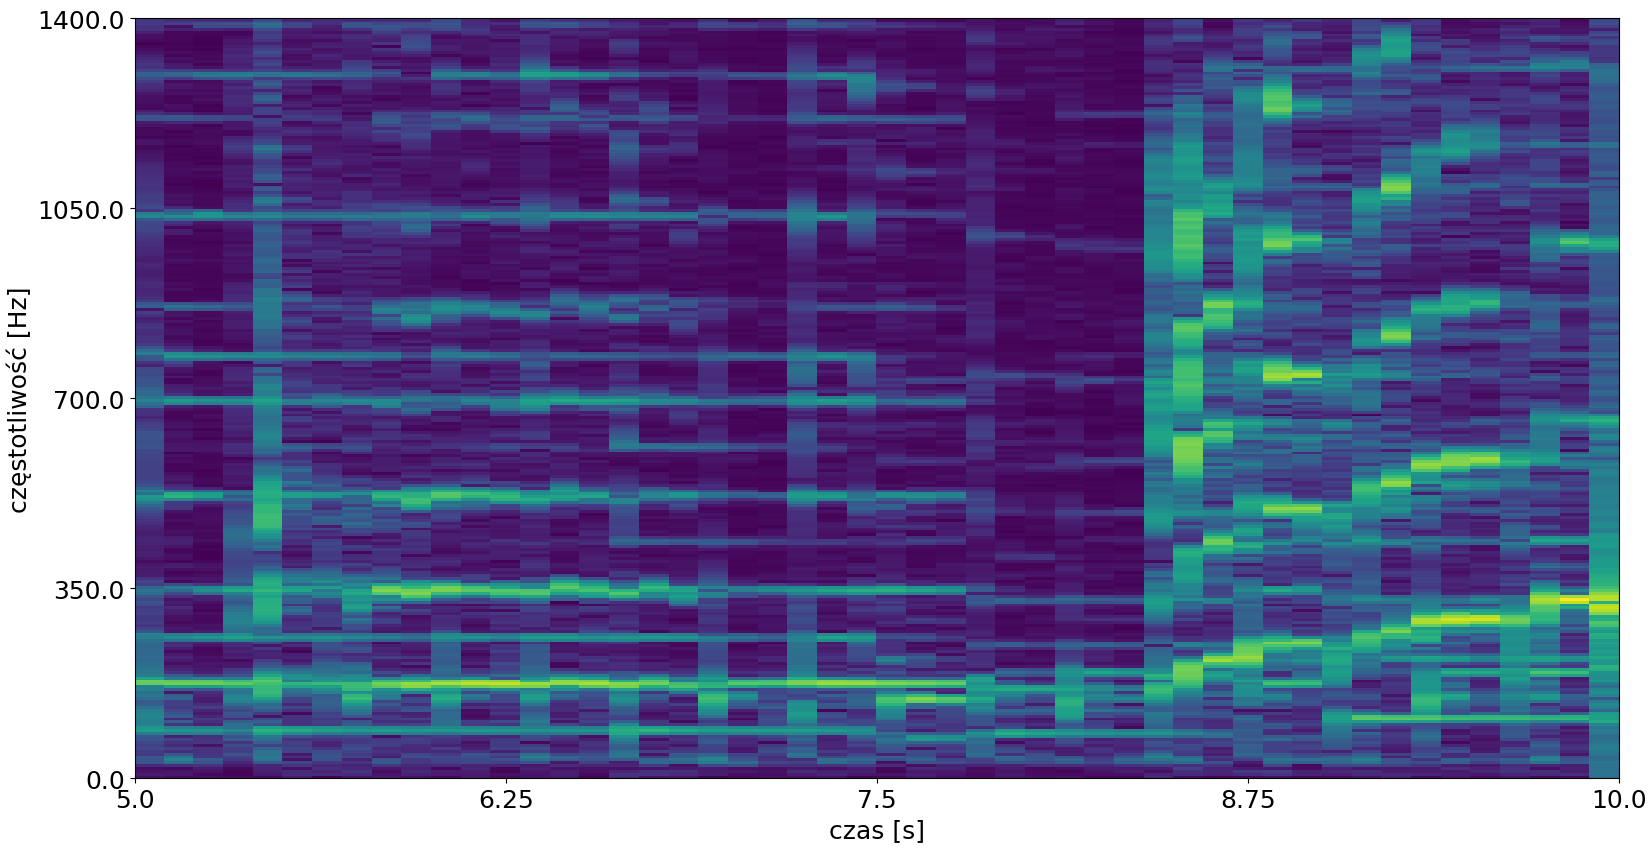
\includegraphics[width=0.9\textwidth]{images/spektrogram}
    \caption{Przykładowy spektrogram (fragment piosenki ,,Yesterday'' zespołu The Beatles).}
    \label{fig:spektrogram}
\end{figure}



\section{Podstawy teorii muzyki}

% głośność i wysokość
Zanim omówione zostaną niezbędne pojęcia z teorii muzyki, należy wspomnieć o tym, jak ludzkie ucho odbiera i interpretuje sygnał dźwiękowy. Posiada on dwie podstawowe cechy: \emph{głośność}\footnote{\cite{lerch_introduction_2012}, s. 71}, która jest związana z amplitudą sygnału, oraz \emph{wysokość}\footnote{\cite{lerch_introduction_2012}, s. 79}, która zależy od częstotliwości. Czym większa amplituda tym dźwięk jest głośniejszy i czym wyższa częstotliwość, tym dźwięk jest wyższy. Warto zwrócić uwagę, że zależność pomiędzy wrażeniem głośności i wysokości a faktycznymi, liczbowymi wartościami amplitudy i częstotliwości jest logarytmiczna. Oznacza to, że aby głośność dźwięku zwiększała się w sposób jednostajny, to jego amplituda musi rosnąć wykładniczo, to samo oczywiście odnosi się do wysokości dźwięku. 

% dźwięki o określonej wysokości
Jeżeli częstotliwości składowe pojedynczego dźwięku, są kolejnymi wielokrotnościami częstotliwości podstawowej, to wtedy da się wyraźnie zauważyć, że dźwięk taki ma określoną wysokość i odpowiada ona właśnie częstotliwości podstawowej\footnote{\cite{lerch_introduction_2012}, s. 79}. Oznacza to, że pojedynczy dźwięk pianina, trąbki czy gitary składa się z bardzo wielu częstotliwości ułożonych zgodnie z opisaną wyżej regułą. Oczywiście istnieją również dźwięki, gdzie układ ten nie jest zachowany. Wtedy trudno jest jednak lub czasem zupełnie niemożliwe, aby określić wysokość dla takiego dźwięku. Rys. \ref{fig:spektrogram_c} przedstawia spektrogram pojedynczego dźwięku zagranego na pianinie. Dźwięk ten ma pojedynczą, określoną wysokość, jednakże posiada wiele częstotliwości składowych. Wszystkie one są wielokrotnościami częstotliwości podstawowej, co wyraźnie da się zauważyć na podstawie jasnych linii na rysunku.

\begin{figure}[htb]
    \centering
    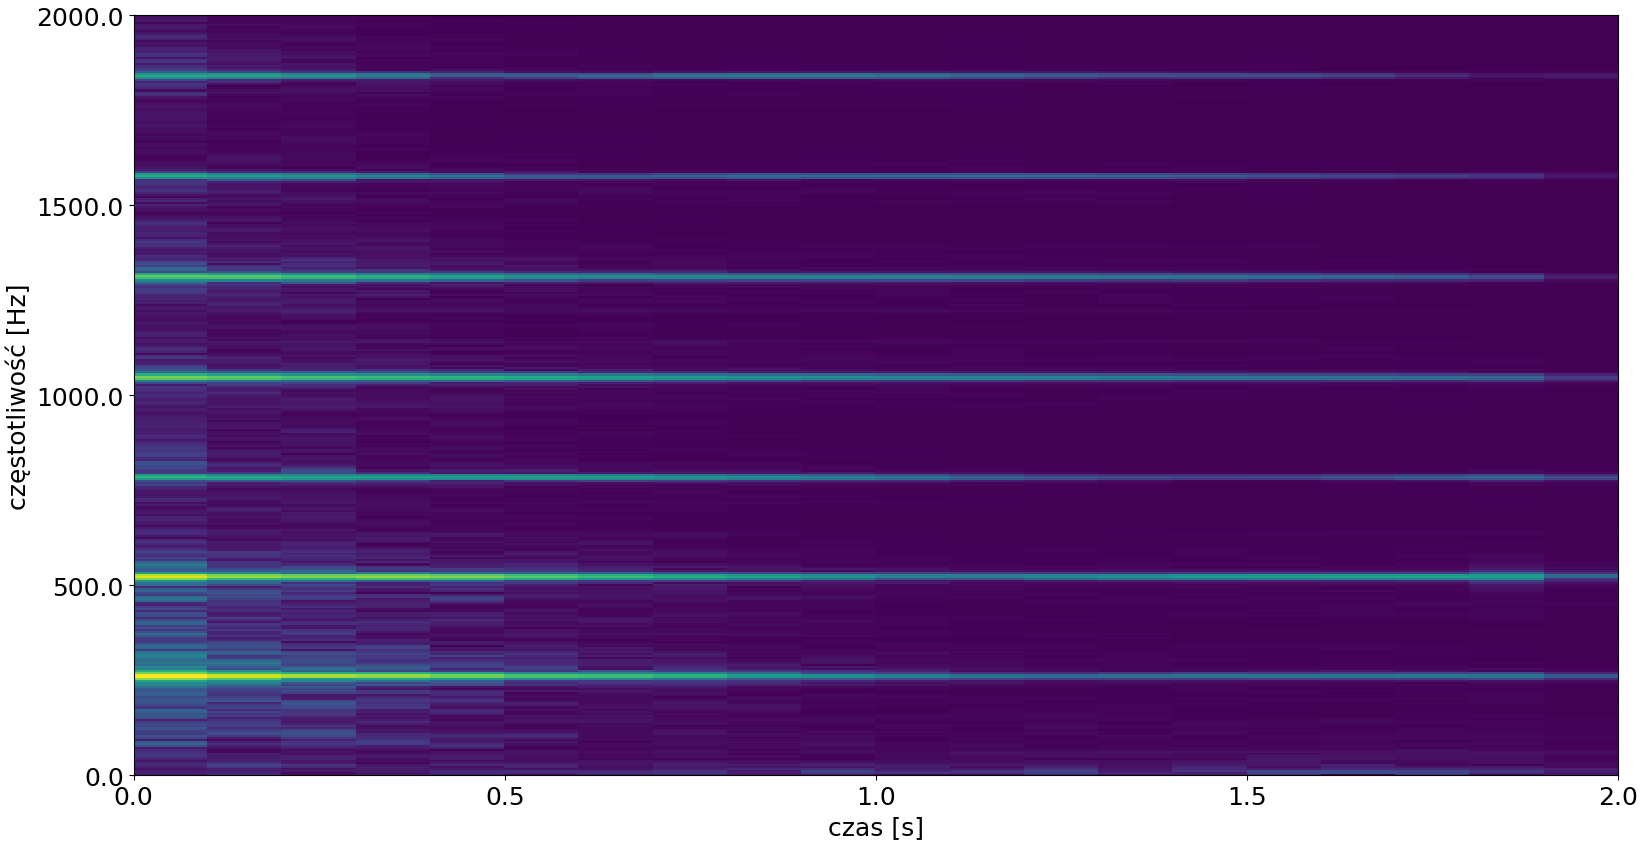
\includegraphics[width=0.9\textwidth]{images/spektrogram_c}
    \caption{Spektrogram pojedynczego dźwięku C zagranego na pianinie.}
    \label{fig:spektrogram_c}
\end{figure}

% oktawy, 12 dźwięków i strój równomiernie temperowany
Istnieje jeszcze jedno istotne zjawisko, związane z ludzką percepcją sygnału dźwiękowego. Mianowicie nasz mózg rozpoznaje jako bardzo podobne do siebie, te dźwięki, których stosunek częstotliwości podstawowych jest potęgą dwójki\footnote{\cite{lerch_introduction_2012}, s. 81}. Ma to bezpośredni wpływ na nazewnictwo dźwięków. Te, których częstotliwości występują w stosunku $2:1$, zostały oznaczone tą samą nazwą literową. Pomiędzy taką parą dźwięków mieści się jeszcze jedenaście innych i w ten sposób dochodzimy do stwierdzenia, że w muzyce wyróżnia się dwanaście różnych nazw dźwięków, które są oddalone od siebie o odległość \emph{półtonu}. Każda taka nazwa odpowiada zatem wielu częstotliwościom podstawowym. Odległość półtonu jest natomiast najmniejszą odległością pomiędzy dźwiękami, jaką stosuje się w muzyce popularnej ,,cywilizacji zachodniej''. Różnica częstotliwości odpowiadająca odległości półtonu rośnie więc, wraz ze zwiększeniem się wartości częstotliwości, w których się poruszamy. System, w którym częstotliwości podstawowe kolejnych dźwięków w oktawie rozłożone są ,,równomiernie'', to znaczy stosunek częstotliwości podstawowych $f_1$ i $f_2$ dowolnych dwóch dźwięków oddalonych od siebie o $N$ półtonów zawsze wyrażony jest wzorem \ref{eq:stroj_rownomiernie_temperowany}, nazywany jest \emph{strojem równomiernie temperowanym}\footnote{\cite{lerch_introduction_2012}, s. 90}, jest to podstawowy strój stosowany dziś w muzyce zachodniej. Istnieją również inne systemy, ale ich omówienie wykracza poza zakres niniejszej pracy.
\begin{equation} \label{eq:stroj_rownomiernie_temperowany}
    \frac{f_1}{f_2} = 2^{N/12}
\end{equation}

% nazwy dźwięków, modyfikatory
Aby móc określić częstotliwości podstawowe odpowiadające danym nazwom dźwięków, trzeba zdefiniować pewną \emph{częstotliwość strojenia}\footnote{\cite{lerch_introduction_2012}, s. 88}. Często przyjmuje się za nią $440$ Hz, która to częstotliwość odpowiada dźwiękowi oznaczanemu literą ,,A''. Wykorzystując wspomnianą częstotliwość i zakładając, że poruszamy się w ramach stroju równomiernie temperowanego, na podstawie wzoru \ref{eq:stroj_rownomiernie_temperowany} można wyliczyć jakie częstotliwości podstawowe przyjmują kolejne dźwięki. Wszystkie dwanaście nazw dźwięków muzycznych wraz z ich oznaczeniami i przykładową, jedną z wielu odpowiadających im częstotliwością podstawową, wyliczonych przy wspomnianych wyżej założeniach, przedstawiono w tab. \ref{tab:nazwy_dzwiekow}. Zaproponowane oznaczenia bazują na \cite{lerch_introduction_2012} i ich budowa sprowadza się do wykorzystania dwóch symboli ,,\#'' oraz ,,b'', które stosuje się również w zapisie nutowym (który nie będzie tutaj omawiany). Pierwszy z nich oznacza podwyższenie dźwięku o pół tonu a drugi obniżenie o pół tonu. Można powiedzieć więc, że w oznaczeniach dźwięków wykorzystuje się $6$ liter oraz $2$ symbole--modyfikatory. Zakładając, że dany modyfikator można wykorzystać wielokrotnie, to pojedynczy dźwięk da się przedstawić na wiele sposobów.  Nazwa dźwięku, jak można się domyślić, również jest związana z obecnością modyfikatora.

\begin{table}[htb]
    \centering
    \caption{Nazwy dźwięków w muzyce.}
    \label{tab:nazwy_dzwiekow}
    \begin{tabular}{|c|c|c|} \hline
        Nazwa & Oznaczenie & Częstotliwość (jedna z wielu) [Hz] \\ \hline
        c       & C     & $261.6$  \\
        cis/des & C\#/Db & $277.2$  \\
        d       & D     & $293.7$  \\
        dis/es  & D\#/Eb & $311.1$  \\
        e       & E     & $329.6$  \\
        f       & F     & $349.2$  \\
        fis/ges & F\#/Gb & $370.0$  \\
        g       & G     & $392.0$  \\
        gis/as  & G\#/Ab & $415.3$  \\
        a       & A     & $440.0$  \\
        ais/b   & A\#/B  & $466.2$  \\
        h       & H     & $493.9$  \\
        c       & C     & $523.2$  \\ \hline
    \end{tabular}
\end{table}

% interwały
Odległość pomiędzy dwoma dźwiękami nazywa się \emph{interwałem muzycznym}\footnote{\cite{lerch_introduction_2012}, s.  83}. Każdy kolejny jest o pół tonu większy od poprzedniego. Nazwy dwunastu pierwszych interwałów wraz z ich oznaczeniami stosowanymi w muzyce przedstawiono w tab. \ref{tab:interwaly}. Ostatni z nich nazywa się \emph{oktawą} i oznacza dźwięk o dwa razy wyższej częstotliwości. Zauważmy, że jest to właśnie ta opisywana wcześniej odległość --- dźwięki oddalone od siebie o oktawę mają tę samą nazwę.  Kolejne oktawy również mają swoje nazwy (mała, wielka, razkreślna itd.), które wykorzystuje się, kiedy trzeba odróżnić dwa dźwięki o tej samej nazwie w dwóch różnych oktawach (np. A razkreślne --- A1).

\begin{table}[htb]
    \centering
    \caption{Interwały muzyczne.}
    \label{tab:interwaly}
    \begin{tabular}{|c|c|c|} \hline
        Nazwa & Oznaczenie & Liczba półtonów \\ \hline
        Pryma           & 0     & 0  \\
        Sekunda mała    & 2>    & 1  \\
        Sekunda wielka  & 2     & 2  \\
        Tercja mała     & 3>    & 3  \\
        Tercja wielka   & 3     & 4  \\
        Kwarta czysta   & 4     & 5  \\
        Tryton          & 4<    & 6  \\
        Kwinta czysta   & 5     & 7  \\
        Seksta mała     & 6>    & 8  \\
        Seksta wielka   & 6     & 9  \\
        Septyma mała    & 7     & 10 \\
        Septyma wielka  & 7<    & 11 \\
        Oktawa czysta   & 8     & 12 \\ \hline
    \end{tabular}
\end{table}

% akord
Jednoczesne brzmienie więcej niż dwóch dźwięków nazywa się \emph{akordem muzycznym}\footnote{\cite{lerch_introduction_2012}, s. 86}. Składa się więc on z (przynajmniej dwóch) interwałów, które znajdują się między parami dźwięków. Zależnie od interwałów, stanowiących ich podstawowy budulec, akordy mają zupełnie różne brzmienie i charakter. Akordy rozróżnia się więc po ich bazowym dźwięku i po ich typie. Wyróżnić można wiele rodzajów akordów, ale na potrzeby niniejszej pracy najważniejsze są dwa z nich.  Pierwszy to tzw. \emph{akord majorowy}, który zawiera kolejno tercję wielką i tercję małą, a drugi to akord minorowy, który zawiera te same interwały, ale w odwrotnej kolejności. Pierwszy ma charakter radosny, a drugi smutny i melancholijny. Zarówno akordy pierwszego, jak i drugiego typu mogą być zbudowane na każdym z dwunastu dźwięków. 

% dalej o akordach
Aby zbudować akord trzeba wybrać dźwięk bazowy, czyli tzw. podstawę akordu. Dla przykładu weźmy dźwięk A. Następnie trzeba obliczyć, jakie dźwięki są oddalone o odpowiednie interwały. Jeżeli budujemy akord majorowy, to kolejnymi dźwiękami tego akordu są C\# oraz E. Jeżeli budujemy akord minorowy, to będą to C i E. Jak widać, różnią się tylko jednym dźwiękiem. Pierwszy z opisanych akordów nazywa się \emph{A-dur} a drugi \emph{a-moll}. W praktyce te trzy lub więcej dźwięków nie muszą być umieszczone w ramach pojedynczej oktawy. Mogą występować w różnych oktawach i mogą się w nich powtarzać. Budowę kilku przykładowych akordów przedstawiono w tab. \ref{tab:przykladowe_akordy}. Jak łatwo zauważyć, nazwy akordów majorowych tworzy się poprzez dodanie sufiksu ,,dur'' do podstawy akordu, a nazwy akordów minorowych poprzez dodanie sufiksu ,,moll''.

\begin{table}[htb]
    \centering
    \caption{Przykładowe akordy muzyczne.}
    \label{tab:przykladowe_akordy}
    \begin{tabular}{|c|c|c|} \hline
        Nazwa akordu & Nazwy dźwięków składowych \\ \hline
        A-dur   & A  C\# E  \\
        g-moll  & G  B  D  \\
        F\#-dur  & F\# A\# C\# \\
        b-moll  & B  Db F  \\ \hline
    \end{tabular}
\end{table}

Na końcu warto jeszcze podkreślić, że widmo częstotliwościowe pojedynczego akordu, nawet jeśli
składa się on tylko z $3$ dźwięków, będzie kilka razy bardziej złożone niż widmo pojedynczego
dźwięku. Wynika to z faktu, że każdy dźwięk budujący akord ma poza częstotliwością podstawową wiele
wyższych częstotliwości składowych. Przykładowy spektrogram zagranego na pianinie akordu C-dur
zaprezentowano na rys. \ref{fig:spektrogram_cdur}.

\begin{figure}[htb]
    \centering
    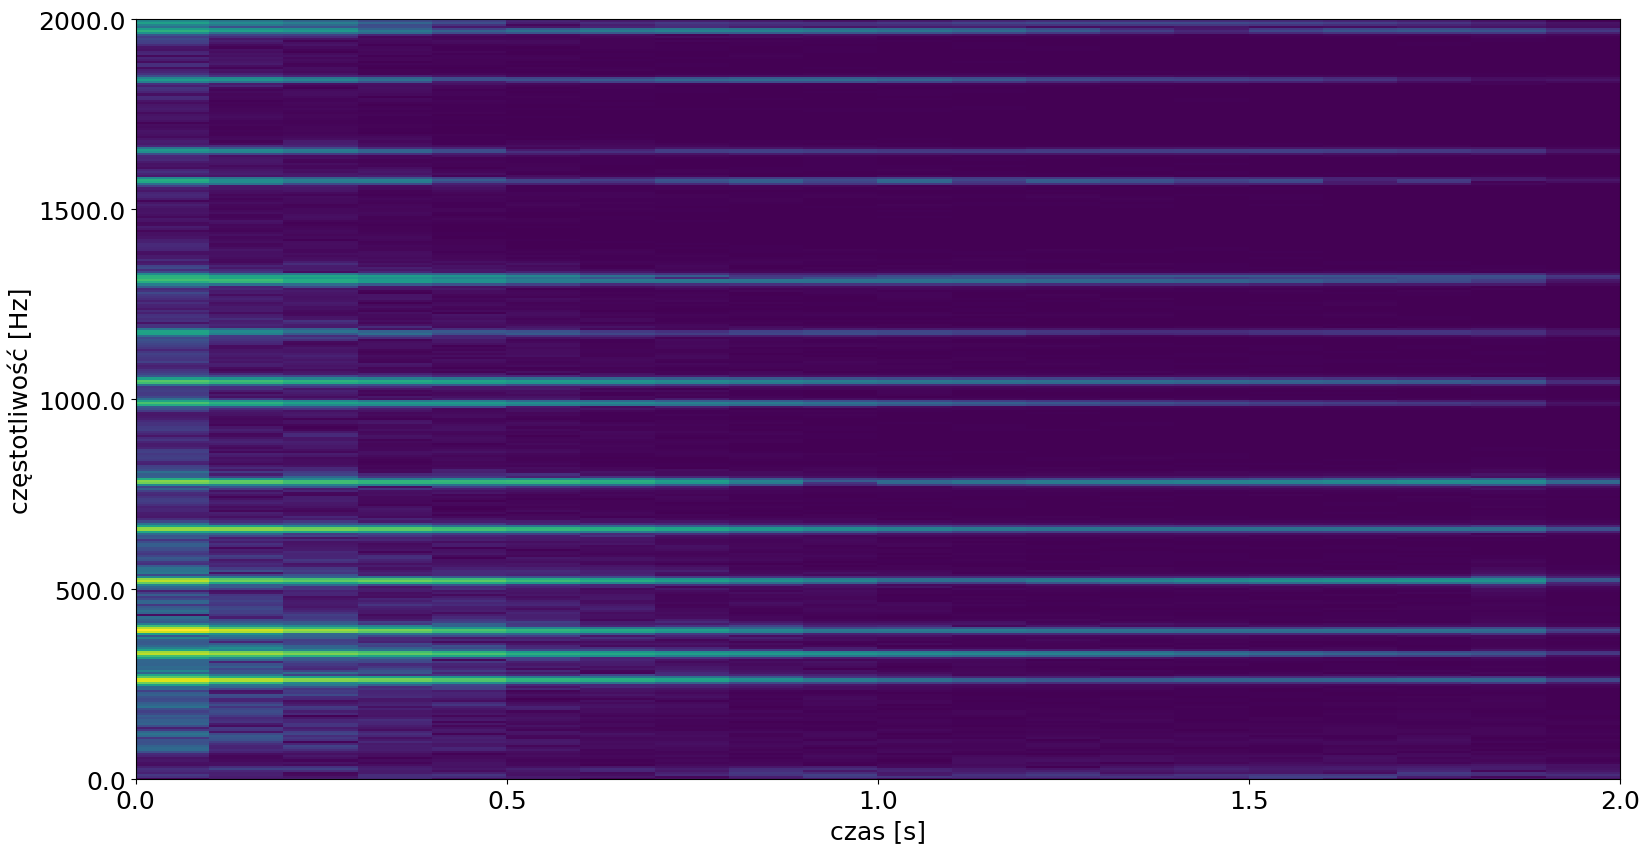
\includegraphics[width=0.9\textwidth]{images/spektrogram_cdur}
    \caption{Spektrogram akordu C-dur zagranego na pianinie.}
    \label{fig:spektrogram_cdur}
\end{figure}



\section{Podstawy analizy akordów muzycznych}

Jak wspominano we wstępie, pierwsze metody analizy akordów muzycznych były oparte jedynie na narzędziach cyfrowego przetwarzania sygnału. Oznacza to, że w celu zidentyfikowania akordu brzmiącego w danym fragmencie utworu, wykonywano szereg jasno zdefiniowanych obliczeń, mających przyporządkować dany fragment do któregoś z wcześniej zdefiniowanej grupy akordów. Metoda tego rodzaju wymaga eksperta znającego się na muzyce oraz matematyce, który przygotuje odpowiedni algorytm na podstawie swojej wiedzy.

Najbardziej oczywiste i bezpośrednie podejście do tematu analizy akordów przedstawione zostało na schemacie \ref{fig:rozpoznawanie_stare_1}. Dla fragmentu utworu, w którym chcemy zidentyfikować akord, przeprowadzona zostaje analiza częstotliwościowa (np. DFT). Następnie poszczególne składowe są zamieniane na odpowiadające im nazwy dźwięków (np. $440$ Hz jest zamienianie na dźwięk $a^1$). Ostatecznie na podstawie zbioru reguł wyodrębnione nazwy dźwięków są zamieniane na pewien odpowiadający im akord.

\begin{figure}[htb]
    \centering
    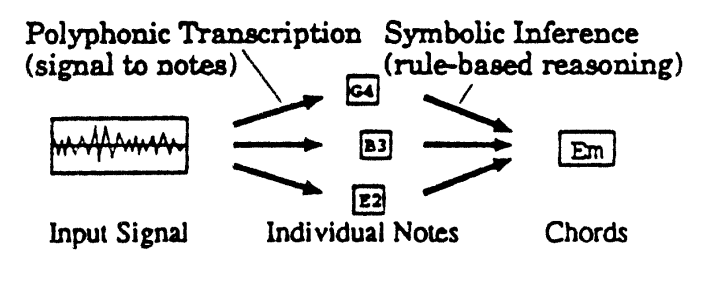
\includegraphics[width=0.9\textwidth]{images/rozpoznawanie_stare_1}
    \caption{Najprostsze podejście do rozpoznawania akordów muzycznych \cite{fujishima_realtime_1999}.}
    \label{fig:rozpoznawanie_stare_1}
\end{figure}

Fujishima \cite{fujishima_realtime_1999} w swoim artykule z roku 1999 zaproponował usprawnienie tej metody, wprowadzając strukturę zwaną PCP (ang. \emph{Pitch Class Profile}). Jest to wektor dwunastu wartości, po jednej dla każdego półtonu. Każdy element tego wektora zawiera sumę natężeń składowych sygnału, które odpowiadają danemu dźwiękowi. Po zbudowaniu PCP wykonywany jest odpowiedni algorytm dopasowania wzorców, który ma na celu wybrać ,,najbardziej podobny'' element z wcześniej zdefiniowanego słownika akordów. Aby więc pomysł mógł zadziałać, wcześniej trzeba przygotować szablon (również w postaci wektora PCP) dla każdego rodzaju akordu, który chcemy móc zidentyfikować. Cały proces został zaprezentowany na rys. \ref{fig:rozpoznawanie_stare_2}. Zaproponowany tutaj wektor PCP był później wielokrotnie wykorzystywany w innych pracach, które rozszerzały tę podstawową metodę o bardziej złożone algorytmy.

\begin{figure}[htb]
    \centering
    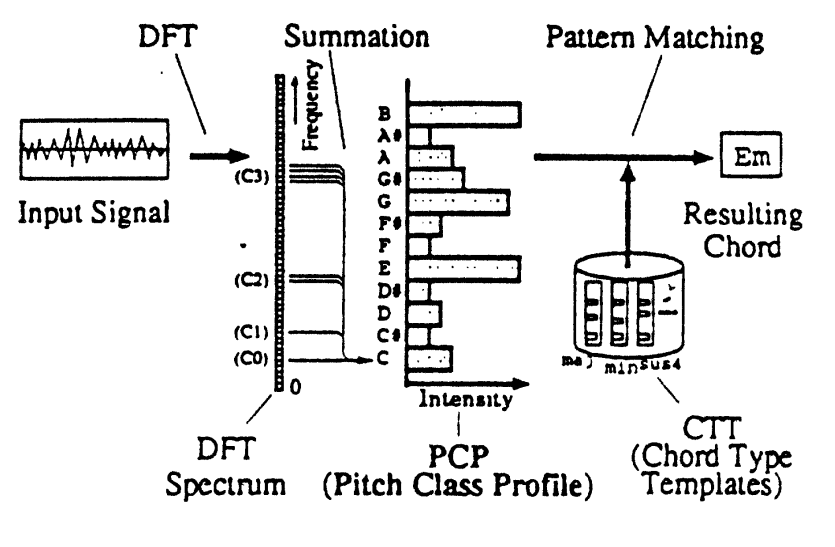
\includegraphics[width=0.9\textwidth]{images/rozpoznawanie_stare_2}
    \caption{Rozpoznawanie akordów muzycznych w oparciu o PCP \cite{fujishima_realtime_1999}.}
    \label{fig:rozpoznawanie_stare_2}
\end{figure}

\chapter{Zbiór danych} \label{chapter:dataset}

% pamiętać, żeby opisać wszystkie kroki, wszystkie SKRYPTY (koncepcję i~algorytmy opisać szczegółowo,
% szczegóły techniczne, jak co zwraca, co przyjmuje dana funkcja pominąć), zerknąć na COMMITY

% potrzeba danych!
Pierwszym i~jednocześnie najważniejszym etapem w~tworzeniu rozwiązania opartego o~uczenie maszynowe jest zgromadzenie odpowiedniego zbioru danych. Jest to etap kluczowy, co wydaje się oczywiste po uwzględnieniu natury tychże algorytmów --- wynajdują one pewne reguły na bazie podanych przykładów.

% potrzeba danych oznaczonych (jak zawsze) i~nieoznaczonych (bo pomogą a~są)
Głęboki sieci neuronowe, co do zasady potrzebują ,,dużo'' (zazwyczaj wiele milionów) przykładów uczących, aby móc znaleźć poprawne reguły i~wzorce --- aby nauczyć się odpowiedniej ekstrakcji cech. W~celu wytrenowania sieci do konkretnego zadania (np. do klasyfikacji obrazów), potrzeba zbioru zawierającego dane wejściowe do modelu i~oczekiwane dane wyjściowe z~modelu. Takie uczenie na podstawie przykładów oznaczonych (ze znaną wartością oczekiwaną) to \emph{uczenie nadzorowane}. Często jednak ilość danych oznaczonych jest ograniczona, można wtedy wykorzystać dane bez oznaczeń w~różnych algorytmach \emph{uczenia nienadzorowanego}, aby nauczyć sieć struktury tych danych, bez ukierunkowania na konkretne zadanie. Dopiero później wykorzystuje się mniejszą ilość danych oznaczonych, aby dotrenować sieć (ang. \emph{fine-tuning}) i~nauczyć ją rozwiązywać dany problem.

% co zawiera ten rozdział - od szukania danych do wejścia do sieci + opis skryptów
W~ramach niniejszej pracy, ze względu na ograniczoną ilość danych oznaczonych, zastosowane zostało właśnie powyższe podejście. Do przeprowadzenia eksperymentów potrzebne były dwa zbiory: pierwszy to ,,niewielki'' zbiór danych oznaczonych a~drugi to ,,zdecydowanie większy'' zbiór danych bez oznaczeń. W~tym rozdziale opisany został proces pozyskiwania obu zbiorów danych z~ogólnie dostępnych źródeł. Zawarto tutaj opis wszystkich kroków wykonanych w~celu przygotowania danych do treningu sieci, poczynając od wyszukiwania oznaczeń utworów muzycznych i~przygotowania parsera dla plików z~tymi oznaczeniami, poprzez automatyczne wyszukiwania i~pobieranie odpowiednich plików z~nagraniami muzycznymi, aż po wstępne przetwarzanie danych do formatu odpowiedniego dla sieci neuronowej. Dodatkowo rozdział ten, poza opisem zastosowanych rozwiązań, zawiera również ogólny opis implementacji tychże rozwiązań, którą to implementację stanowią skrypty języka Python.

% od początku do uzyskania wszystkich oznaczeń ('data/chordlab') oraz pierwszego indeksu (skrypt 01)
\section{Pozyskanie zbiorów danych z~oznaczeniami akordów}
\sectionmark{Pozyskanie oznaczeń akordów}

% trudno o~dane oznaczone w~ACR
Ze względu na powszechną dostępność dużej ilości danych w~Internecie, zgromadzenie zbioru danych nieoznaczonych nie stanowiło szczególnego problemu. Znacznie trudniejsze okazało się zgromadzenie zbioru danych oznaczonych. Zadanie rozpoznawania akordów muzycznych, mimo iż będące jednym z~głównych zadań z~dziedziny MIR, jest jednak bardzo mało popularne w~stosunku do takich zadań jak klasyfikacja, czy segmentacja obrazów. Jest to również po prostu znacznie mniej przydatne w życiu codziennym i~znacznie mniej się w~tę dziedzinę inwestuje. Ponadto przygotowanie oznaczeń akordów do utworów muzycznych wymaga specjalistycznej wiedzy muzycznej, praktyki muzycznej i~dużo czasu. Oznaczenia powstałe w~ten sposób nadal pozostają subiektywne i~będą się często różnić, w~zależności od osoby, która utwory oznaczała. Wszystkie wymienione powody są przyczyną tego, że nie przygotowano więcej niż kilka publicznie dostępnych zbiorów oznaczeń akordów muzycznych, które mogą zostać wykorzystane do treningu modeli uczenia maszynowego.

% zbiory są takie, co to inni wykorzystywali
W~ramach niniejszej pracy przestudiowana została literatura z~dziedziny rozpoznawania akordów za pomocą sieci neuronowych --- większość wykorzystywanych przez badaczy zbiorów danych udało się odnaleźć i~wykorzystać. Zostały one szczegółowo opisane poniżej. Każdy zbiór oznaczeń został pobrany, odpowiednio oczyszczony (wybrane zostały tylko niezbędne pliki) i~zapisany w~repozytorium projektu (w katalogu \url{data/chordlab}). Po przeanalizowaniu struktury zbiorów stworzony został pierwszy skrypt przygotowujący dane --- \url{src/dataset_scripts/01-generate_index_of_chordlab.py} --- który, w~postaci pliku \filetype{csv}, generuje jeden wspólny indeks (\url{data/index.csv}) dla wszystkich zbiorów, tak że mogą one być już traktowane jako jeden zbiór danych. Fragment tego indeksu został przedstawiony w~Tab. \ref{tab:indeks_01}.

\begin{table}
    \centering
    \caption{Fragment indeksu zbioru danych po pierwszym etapie jego tworzenia.}
    \label{tab:indeks_01}
    \makebox[\textwidth][c]{
    {\scriptsize \ttfamily \begin{tabular}{rllllr}
    \hline
    & filepath & song & artist & subset & album \\
    \hline
     0 & ./data/\ldots/1999\_dt.clt                      & 1999                      & Prince                      & rs200 & nan \\ 
     1 & ./data/\ldots/a\_change\_is\ldots & A~Change Is Gonna Come    & Sam Cooke                   & rs200 & nan \\
     5 & ./data/\ldots/all\_along\_t\ldots & All Along the Watchtower  & The Jimi Hendrix Experience & rs200 & nan \\
     6 & ./data/\ldots/all\_apologie\ldots & All Apologies             & Nirvana                     & rs200 & nan \\
     7 & ./data/\ldots/all\_i\_have\ldots & All I~Have to Do Is Dream & The Everly Brothers         & rs200 & nan \\
    \hline
    \end{tabular}}}
\end{table}

Trzeba jeszcze zaznaczyć, że wszystkie te zbiory są udostępniane za darmo, ale jedynie jako same pliki tekstowe z~oznaczeniami akordów. Pliki z~nagraniami muzycznymi, ze względu na prawa autorskie, nie są udostępniane. Pozyskanie odpowiednich nagrań stanowi osobny problem, opisany w~dalszej części rozdziału.

\subsection{Zbiór Isophonics}

% ogólny opis, jakie i~ile utworów, format zapisu
\emph{Isophonics} to właściwie nazwa serwisu internetowego\footnote{\url{www.isophonics.net/about}}, prowadzonego przez zespół naukowy \emph{Centre for Digital Music} z~londyńskiego Uniwersytety Królowej Marii\footnote{\url{https://c4dm.eecs.qmul.ac.uk/}}. Jest to duża i~popularna na cały świat jednostka naukowa specjalizująca się w~badaniach dotyczących przetwarzania muzyki cyfrowej. W~serwisie tym dostępne są między innymi oprogramowanie oraz zbiory danych związane z~różnymi aspektami przetwarzania sygnałów muzycznych.  Można tam znaleźć najbardziej popularny i~zapewne najstarszy zbiór z~oznaczeniami akordów muzycznych, przygotowany dla 180 piosenek zespołu \emph{The Beatles}, szczegółowo opisany w \cite{harte_towards_nodate}. Zbiór ten rozrósł się o~oznaczenia dla 20 utworów \emph{Queen}, 18 utworów \emph{Zweieck} i~7 utworów \emph{Carole King}. Wykorzystany format zapisu oznaczeń akordów również jest opisany w \cite{harte_towards_nodate} i~jest wykorzystywany praktycznie jako standard, również w~przypadku innych zbiorów danych. Warto wspomnieć jeszcze, że jest to pierwszy referencyjny zbiór wykorzystywany w~konkursie MIREX\footnote{\url{https://www.music-ir.org/mirex/wiki/MIREX_HOME}}, w~zadaniu automatycznego rozpoznawania akordów.

% pobieranie i~indeksowanie
Zbiór \emph{Isohponics} jest dostępny do pobrania ze strony projektu w~postaci skompresowanych archiwów \filetype{tar} (osobny plik dla każdego z~czterech artystów). Każde z~tych archiwów ma taką samą strukturę i~zawiera nie tylko oznaczenia akordów, dostępne w~różnych formatach, ale również inne informacje o~utworach, jak zmiany tonacji czy segmentacje strukturalne. Spośród wszystkich tych plików wykorzystane zostały jedynie oznaczenia akordów w~postaci plików \filetype{lab} --- pozostałe pliki zostały usunięte. Pliki z~oznaczeniami akordów uporządkowane są w~takiej strukturze katalogów, gdzie nazwy katalogów na kolejnych poziomach zagłębienia odpowiadają kolejno nazwie artysty, nazwie albumu (dla The Beatles poprzedzonej dodatkowo liczbą porządkową) i~numerowi wraz z~nazwą konkretnego utworu. Zbiór ten nie posiada żadnego dodatkowego indeksu, przy tworzeniu własnego indeksu zostały więc wykorzystane nazwy katalogów.

% poprawki i~zapisanie w~projekcie
Jedyne zmiany, jakie zostały wprowadzone w~oznaczeniach akordów po pobraniu ich z~Internetu, poza usunięciem niewykorzystywanych plików, dotyczą artystki Carole King. Polegały one na dostosowaniu kilku skrótów typów akordów, które występowały jedynie tutaj, a~były niezgodne z~przyjętą w \cite{harte_towards_nodate} konwencją. Wszystkie oznaczenia zbioru \emph{isohponics}, po przeprowadzeniu opisanych powyżej operacji, zostały zapisane w~repozytorium projektu, w~katalogu \url{data/chordlab/isophonics}.


\subsection{Zbiór McGill Billboard}

% ogólny opis, jakie i~ile utworów, format zapisu
Zbiór \emph{McGill Billboard} \cite{burgoyne_expert_2011} został stworzony przez grupę DDMAL (ang. \emph{Distributed Digital Music Archives \& Libraries Lab})\footnote{\url{https://ddmal.music.mcgill.ca/}} z~kanadyjskiego \emph{McGill University}. Jak nazwa wskazuje, zajmują się oni różnymi projektami związanymi z~przetwarzaniem muzyki, w~tym tworzą i~utrzymują ten prawdopodobnie największy, dostępny publicznie zbiór danych z~różnymi typami oznaczeń utworów, takimi jak akordy, struktura, instrumenty i~tempo. Lista utworów wybranych do tego zbioru została zbudowana z~1300 utworów, losowo wybieranych z~rankingów serwisu \emph{Billboard}\footnote{\url{www.billboard.com}}. W~praktyce, ponieważ niektórych utworów nie udało się twórcom znaleźć, zbiór ten zawiera 890 utworów muzyki popularnej, przy czym zdarzają się takie, które się powtarzają. Oznaczenia akordów są wyrównane w~czasie zgodnie z~częstotliwością występowania taktów. Format tych oznaczeń bazuje ściśle na \cite{harte_towards_nodate} (tak jak \emph{isophonics}), jedyna różnica polega na wprowadzeniu kilku dodatkowych skrótów typów akordów.  Podobnie jak w~przypadku innych zbiorów z~oznaczeniami akordów, twórcy tego zbioru nie mogli udostępnić nagrań muzycznych. Jednakże w~tym przypadku udostępnione zostały dwa zestawy cech dla wszystkich akordów: \emph{non-negative-least-squares chroma vectors} oraz \emph{Echo Nest features}, które mogą zostać wykorzystane jako wejście do modeli ML, nie były jednak użyte w~ramach niniejszej pracy.

% pobieranie i~indeksowanie
Zbiór \emph{McGill Billboard} dostępny jest do pobrania\footnote{\url{https://ddmal.music.mcgill.ca/research/The_McGill_Billboard_Project_(Chord_Analysis_Dataset)/}} w~postaci skompresowanych (na kilka sposobów) archiwów \filetype{tar}. Dostępne są pliki ze wspomnianymi powyżej dwoma zestawami dźwiękowych cech utworów, dostępny jest zestaw wszystkich oznaczeń we własnym formacie twórców zbioru, oraz zestaw oznaczeń samych akordów, w~postaci plików \filetype{lab}.  Do niniejszej pracy wykorzystany został jedynie ten ostatni zestaw, zawierający pliki \filetype{lab}. Pobrane archiwum zawiera główny katalog \url{McGill-Billboard}, w~którym znajduje się 890 katalogów nazwanych liczbowymi identyfikatorami utworów ze zbioru. Każdy taki katalog zawiera jeden plik \url{full.lab} z~oznaczeniami akordów. Twórcy zbioru dostarczają również indeks w~postaci pliku \filetype{csv}, wiążący identyfikatory utworów z~tytułem, artystą (album nie jest podany) i~innymi informacjami związanymi z~rankingiem, z~którego pochodzi utwór. Indeks ten jest niestety bardzo wybrakowany i~dla wielu utworów brakuje wpisu o~tytule lub artyście. Po wybraniu tych przypadków, dla których znany jest tytuł i~artysta zostało jedynie $596$ utworów. Tabela ta została wykorzystana do przygotowania własnego indeksu.

% poprawki i~zapisanie w~projekcie
Pobrane oznaczenia akordów nie wymagały właściwie żadnych poprawek. Cały katalog \url{McGill-Billboard} został przeniesiony do repozytorium projetu, do katalogu \url{data/chordlab/mcgill_billboard}.

\subsection{Zbiór Robbie Williams}

% ogólny opis, jakie i~ile utworów, format zapisu
Zbiór \emph{Robbie Williams} \cite{giorgi_automatic_2013} składa się z~oznaczeń akordów oraz tonacji dla pierwszych pięciu albumów Robbiego Williamsa. Został przygotowany przez włoskich naukowców z~Politechniki w~Mediolanie na potrzeby uczenia systemu automatycznego rozpoznawania akordów.  Oznaczenia są zgodne z \cite{harte_towards_nodate}. W~sumie dokładne oznaczenia akordów i~tonacji przygotowano dla 65 utworów.

% pobieranie i~indeksowanie
Zbiór ten dostępny jest do pobrania ze strony\footnote{\url{https://www.researchgate.net/publication/260399240_Chord_and_Harmony_annotations_of_the_first_five_albums_by_Robbie_Williams}} w~postaci archiwum zip. Znajduje się w~nim katalog \url{RobbieWilliamsAnnotations}, który zawiera dwa główne podkatalogi: \url{chords} i \url{keys}. W~każdym z~tych podkatalogów znajduje się po pięć podkatalogów (po jednym na album). W~każdym katalogu z~albumem znajdują się pliki \filetype{txt} z~oznaczeniami akordów w~formacie \filetype{lab}. Zbiór ten nie posiada żadnych dodatkowych metadanych --- własny indeks wygenerowany został na podstawie znormalizowanych nazw katalogów.

% poprawki i~zapisanie w~projekcie
Pobrane oznaczenia znowu nie wymagały żadnych poprawek. Zawartość katalogu \url{RobbieWilliamsAnnotations/chords/} została przeniesiona do repozytorium projektu, do katalogu \url{data/chordlab/robbie_williams}.

\subsection{Zbiór RS200}

% ogólny opis, jakie i~ile utworów, format zapisu
Zbiór \emph{RS200} \cite{de_clercq_corpus_2011} został stworzony przez dwóch badaczy z~amerykańskiej uczelni muzycznej \emph{Eastman School of Music} w~Rochester. Powstał on na bazie listy \emph{500 Greatest Songs of All Time} z~magazynu \emph{Rolling Stone}. Początkowo zawierał jedynie 100 utworów i~w takiej formie został wykorzystany w~oryginalnej publikacji, gdzie autorzy analizowali częstość występowania różnych akordów i~ich progresji. Utwory te zostały wybrane tak, aby pochodziły z~wielu różnych dekad. Z~czasem zbiór został rozszerzony do 200 utworów i~w takiej formie jest dostępny do dzisiaj. Każdy z~dwóch twórców, niezależnie od drugiego, przygotował swoje oznaczenia dla wszystkich 200 utworów. Oznaczenia te zawierają nie tylko akordy, ale również transkrypcję melodii, informacje o~tempie i~tekstach utworów. Format zapisu oznaczeń akordów został opracowany przez twórców tego zbioru danych i~różni się zdecydowanie od sposobu oznaczeń stosowanego w~pozostałych zbiorach.  Bardziej szczegółowo został opisany w~dalszej części rozdziału, ale ogólnie opiera się on na rekurencyjnej składni, pozwalającej łatwo reprezentować pewne schematy i~powtórzenia w~strukturze utworów. Same oznaczenia akordów są również ustalone przez tych autorów i~bazują na liczbach rzymskich, które prezentują informacje względem tonacji całego utworu. Mamy więc tutaj do czynienia z~podejściem zupełnie innym, od przyjętego dla pozostałych zbiorów danych.

% pobieranie i~indeksowanie
Zbiór ten dostępny jest do pobrania ze strony\footnote{\url{http://rockcorpus.midside.com/harmonic_analyses.html}}. Właściwie autorzy oferują trzy formaty, z~których ostatni jest już rozwinięty do postaci zbliżonej do plików \filetype{lab}. Główna różnica to wspomniany powyżej sposób oznaczania konkretnych akordów. Po pobraniu i~rozpakowaniu archiwum \emph{zip} znaleźć można pojedynczy katalog \url{rs200_harmony_clt}, który zawiera pliki z~rozszerzeniem \emph{clt}, po dwa dla każdego utworu, jeden z~sufiksem ,,dt'' a~drugi ,,tdc'' (od nazwisk autorów). Ze względu na to, że oznaczenia jednego z~autorów były znacznie bardziej uporządkowane i~prostsze, a~kwestia różnic w~oznaczeniach dwóch różnych osób nie jest szczególnie związana z~tematem niniejszej pracy, wybrane zostały jedynie oznaczenia z~sufiksem ,,dt''. Jeżeli chodzi o~indeksowanie plików z~oznaczeniami, to autorzy dostarczają plik \filetype{txt} z~opisem wszystkich plików z~oznaczeniami, w~tym z~tytułem utworu, rokiem wydania i~nazwiskiem artysty. Plik ten, po wprowadzeniu kilku niezbędnych poprawek (literówki i~pomyłki w~nazwach, odniesienia do nieistniejących plików), został wykorzystany do generowania głównego indeksu utworów.

% poprawki i~zapisanie w~projekcie
Wybrane pliki z~sufiksem ,,dt'' nie wymagały już więcej poprawek. Zostały wszystkie przeniesione do katalogu \url{data/chordlab/rs200}.

\subsection{Zbiór RWC POP}

% ogólny opis, jakie i~ile utworów, format zapis
Zbiór RWC POP \cite{goto_rwc_nodate} stanowi część większego zbioru o~nazwie RWC (ang. \emph{Real World Computing}) Music Database\footnote{\url{https://staff.aist.go.jp/m.goto/RWC-MDB/}}, stworzonego przez Real World Computing Partnership (RWCP) w~Japonii. Jest to oczyszczony z~praw autorskich, dostępny za darmo (trzeba pokryć jedynie koszty kopiowania i~dostawy) wielkoskalowy zbiór 315 utworów muzycznych, podzielonych na 5~zestawów o~różnym zastosowaniu, jak rozpoznawanie gatunku czy instrumentu muzycznego. Jednym z~tych zestawów jest właśnie Popular Music Database zawierający 100 utworów muzyki popularnej --- 20 w~stylu popularnej muzyki zachodniej z~lat 80. (w języku angielskim) i~80 w~stylu popularnej muzyki japońskiej, z~lat 90. (w języku japońskim). Właściwie zbiór ten, poza możliwością uzyskania darmowego i~legalnego dostępu do nagrań dźwiękowych, nie jest przydatny dla zadania rozpoznawania akordów, ponieważ nie zawiera oznaczeń akordów. Te zostały jednak przygotowane dla wszystkich 100 utworów przez studentów uniwersytetu w~Nowym Jorku z~Music and Audio Research Lab. Format tych oznaczeń jest ponownie zgodny z \cite{harte_towards_nodate}. W~ramach niniejszej pracy wykorzystane zostały właśnie te oznaczenia.  Dla uproszczenia i~zautomatyzowania całego procesu przygotowania danych, nagrania muzyczne próbowano pozyskać tą samą metodą jak w~przypadku pozostałych zbiorów danych.

% pobieranie i~indeksowanie
Oznaczenia akordów do zbioru RWC POP są dostępne za darmo do pobrania w~Internecie jako repozytorium git w~serwisie GitHub\footnote{\url{https://github.com/tmc323/Chord-Annotations}}. Bezpośrednio w~repozytorium znajduje się katalog \url{RWC_Pop_Chords}, który zawiera pliki z~oznaczeniami akordów w~dwóch formatach: \url{svl} oraz \filetype{lab}. Wykorzystane zostały jedynie pliki \filetype{lab}. Nazwy tych plików zawierają liczbowe identyfikatory poszczególnych nagrań. Aby przygotować indeks i~pozyskać informacje o~tytułach, nazwach albumów i~nazwiskach artystów ze strony projektu\footnote{\url{https://staff.aist.go.jp/m.goto/RWC-MDB/rwc-mdb-p.html}} skopiowana została tabela ze wszystkimi tymi informacjami. Tabela ta zapisana została w~pliku \url{data/chordlab/rwc_pop/rwc_pop.txt} i~była wykorzystana w~skrypcie generującym indeks.

% poprawki i~zapisanie w~projekcie
Przygotowane przez nowojorskich studentów oznaczenia nie wymagały żadnych poprawek. Wszystkie pliki \filetype{lab} zostały umieszczone w~katalogu \url{data/chordlab/rwc_pop}.

\subsection{Zbiór Uspop2002}

% ogólny opis, jakie i~ile utworów, format zapis
Zbiór Uspop2002 \cite{berenzweig_large-scale_2004} został przygotowany w~ramach współpracy naukowców z \emph{LabROSA (Laboratory for the Recognition and Organization of Speech and Audio)} z~Uniwersytetu w~Kolumbii, naukowców z~MIT i~naukowców z \emph{HP Labs} w~Cambridge. Jest to zbiór 8752 utworów, pochodzących od 400 różnych artystów, z~706 różnych albumów. Podobnie jak w~przypadku większości wykorzystanych zbiorów danych, oryginalne nagrania muzyczne nie są udostępniane bezpośrednio --- dostępne są jedynie wyekstrahowane wcześniej cechy MFCC. Zbiór ten został stworzony na potrzeby badań nad miarami podobieństwa między utworami, autorzy nie dostarczają więc oznaczeń akordów. Na szczęście studenci z~Nowego Jorku, poza przygotowaniem oznaczeń dla zbioru RWC POP, przygotowali również oznaczenia akordów dla 195 utworów z~tego zbioru. Oznaczenia te mają ponownie format plików \filetype{lab}, zgodny z \cite{harte_towards_nodate}. W~ramach niniejszej pracy zbiór Uspop2002 nie był więc wykorzystywany bezpośrednio, a~jedynie jako punkt wyjścia dla twórców wspomnianych 195 plików z~oznaczeniami, które to dopiero były wykorzystane w~niniejszej pracy.

% pobieranie i~indeksowanie
Dokładnie tak jak w~przypadku zbioru RWC POP, oznaczenia są dostępne za darmo do pobrania w~Internecie --- stanowią część tego samego repozytorium w~serwisie GitHub\footnote{\url{https://github.com/tmc323/Chord-Annotations}}. Znajdują się w~katalogu \url{uspopLabels}, który zawiera katalogi nazwane nazwiskami artystów. Każdy z~katalogów artysty zawiera katalogi (zazwyczaj jeden) z~nazwami albumów. Dopiero w~katalogach z~albumami znajdują się pliki \filetype{lab}, zawierające w~nazwie tytuły konkretnych utworów. Nazwy katalogów i~nazwy plików zostały wykorzystane podczas generowania indeksu.

% poprawki i~zapisanie w~projekcie
Ponownie oznaczenia nie wymagały żadnych poprawek. Całą zawartość katalogu \url{uspopLabels} przeniesiono do katalogu projektu \url{data/chordlab/uspop}.

% duplikaty i~podsumowanie
\subsection{Usuwanie duplikatów i~podsumowanie pozyskanych oznaczeń}

Ostatnim etapem przygotowania wspólnego indeksu, opisującego wszystkie pozyskane pliki z~oznaczeniami, jest usunięcie duplikatów. Procedura ta, stanowiąca ostatni fragment skryptu tworzącego indeks, jest następująca:

\begin{enumerate}
    \item Znormalizuj kolumny z~nazwą utworu, artysty i~albumu poprzez zamianę wszystkich wielkich
        liter na małe oraz usunięcie białych znaków z~początku i~końca ciągów tekstowych.
    \item Pogrupuj wszystkie utwory po kluczu składającym się z~tytułu i~nazwy artysty --- grupy te
        zawierają potencjalne duplikaty utworów.
    \item Jeżeli w~grupie występują razem utwory ze znanym albumem i~bez albumu, to usuń wszystkie
        utwory bez albumu.
    \item Jeżeli w~grupie występuje kilka utworów z~tym samym albumem, to zostaw tylko jeden
        (losowy) spośród nich.
\end{enumerate}

W~sumie wszystkich plików z~oznaczeniami udało się zgromadzić 1380. Po etapie usuwania duplikatów pozostało 1268. Tab. \ref{tab:datasets1} prezentuje rozkład wszystkich dostępnych plików z~oznaczeniami między poszczególne, opisane wcześniej zbiory danych.

\begin{table}
    \centering
    \caption{Liczebności plików z~oznaczeniami dla poszczególnych zbiorów danych.}
    \label{tab:datasets1}
    \begin{tabular}{|l|c|c|c|c|c|c|c|} \hline
        Nazwa zbioru & Liczba utworów (z duplikatami) \\ \hline
        Isophonics & 225 (225) \\
        McGill Billboard & 509 (596) \\
        Robbie Williams & 65 (65) \\
        RS200 & 174 (199) \\
        RWC POP & 100 (100) \\
        Uspop2002 & 195 (195) \\
        SUMA & 1268 (1380) \\ \hline
    \end{tabular}
\end{table}


% annotation parser i~implementacja WCSR
\section{Model akordów muzycznych i~parsowanie plików z~oznaczeniami} \label{section:chord_model}
\sectionmark{Model akordów muzycznych}

% potrzeba parsowania - wstęp
Po zgromadzeniu, oczyszczeniu i~zindeksowaniu zbiorów z~oznaczeniami akordów, należało przygotować skrypty parsujące pliki z~tymi oznaczeniami. Wszystkie znalezione zbiory oznaczeń, z~wyjątkiem jednego, są w~formacie \filetype{lab}, który to format został opracowany w \cite{harte_towards_nodate}.  Jest to format bardzo przemyślany i~dopracowany, którego użycie przez wielu niezależnych badaczy potwierdza, że sprawdza się on jako standard. Drugi format, znacznie mniej usystematyzowany, opracowany został na potrzeby zbioru RS200, gdzie autorzy przygotowali własny sposób oznaczania akordów. Aby na końcu wykorzystać zarówno oznaczenia, jak i~nagrania muzyczne do treningu sieci neuronowych, trzeba przetłumaczyć pliki tekstowe z~oznaczeniami, na odpowiednią, zrozumiałą dla komputera strukturę danych. W~ramach tego podrozdziału opisana zostanie najpierw ta struktura, a~następnie algorytm parsowania obu dostępnych formatów oznaczeń akordów. Skrypty pythonowe, które realizują zadanie tłumaczenia oznaczeń w formacie plików tekstowych na odpowiednią strukturę danych, umieszczone zostały w~module \url{src/annotation_parser}.

% Opis modelu akordu - skrypt chord_model.py
\subsection{Model obiektowy reprezentujący akordy muzyczne} \label{subsection:chord_model}

% Podstawowy model obiektowy akordu według Krzyśka
W~ramach niniejszej pracy przygotowany został obiektowy model reprezentujący akord muzyczny. Model ten ma formę zestawu klas pythonowych (w pliku \url{src/annotation_parser/chord_model.py}) i~bazuje ściśle na propozycji \cite{harte_towards_nodate}. Według oryginalnego pomysłu każdy akord reprezentowany jest przez trzy części składowe: podstawę akordu (ang. \emph{root}), interwały składowe (ang. \emph{component intervals}) oraz bas (ang. \emph{bass note}), czyli najniższy dźwięk w~akordzie. Podstawa to po prostu nazwa dźwięku, na którym akord jest zbudowany. Nazwa ta reprezentuje jeden z~dwunastu dostępnych tonów i~na potrzeby tego projektu jest kodowana wartością całkowitą od $0$ do $11$, gdzie $0$ oznacza dźwięk c, $1$ oznacza dźwięk cis, itd. Zarówno interwały składowe akordu, jak i~jego bas są reprezentowane jako interwały w~odniesieniu do podstawy akordu.  Aby zapisać interwał, trzeba przede wszystkim zawrzeć informację o jego stopniu (ang.  \emph{degree}), związanym ze stopniem skali diatonicznej i~pozwalającym przedstawić interwały czyste oraz wielkie. Do przedstawienia pozostałych interwałów (małych, zmniejszonych itd.) trzeba dodać informację o modyfikatorze, który odpowiednio zmniejsza lub zwiększa liczbę półtonów budujących interwał. Te dwie informacje --- stopień i~modyfikator --- reprezentują jednoznacznie interwał i~mogą być zapisane jako dwie wartości całkowite. Ostatecznie akord reprezentowany jest więc przez podstawę (liczba całkowita), jeden interwał oznaczający bas i~listę interwałów składowych.

% tłumaczenie na labelki - potrzeba (do treningu), zasady (z MIREXa) i~nazwy metod (to/from_label)
Powyższy model pozwala jednoznacznie zakodować pojedynczy akord muzyczny w~formie prostej i~zrozumiałej dla pozostałej części programu. Model ten, składający się z~dwóch klas --- \code{Interval} i \code{Chord} --- i~kilku liczb całkowitych, został rozszerzony o~dodatkowe klasy i~metody. Przede wszystkim dodane zostały metody umożliwiające tłumaczenie akordów na etykiety (ang. \emph{labels}) lub inaczej klasy z~predefiniowanego zbioru (słownika). Podczas treningu sieci neuronowej trzeba bowiem zdefiniować skończony i~dyskretny zbiór klas, które sieć ma rozpoznawać. Istnieje wiele sposobów, według których można podzielić wszystkie możliwe akordy na skończoną liczbę klas.  Najprostszy z~nich to podzielenie akordów na 13 klas, 12 odpowiada wszystkim możliwym podstawom akordu a~ostatnia (lub pierwsza) oznacza brak akordu. Innym, najpopularniejszym w~literaturze i~stosowanym również w~ramach niniejszej pracy jest tzw. podział major/minor, czyli 25 klas: klasa 0~oznacza brak akordu, klasy od 1~do 12 oznaczają akordy majorowe o~różnych podstawach, a~klasy od 13 do 24 oznaczają akordy minorowe. Istnieją również inne zestawy klas akordów, nie były one jednak wykorzystywane w~ramach niniejszej pracy, choć przygotowana implementacja pozostawia możliwość łatwego dodawania nowych słowników akordów. Zgodnie z~filozofią stosowaną w~konkursie MIREX\footnote{\url{https://www.music-ir.org/mirex/wiki/2021:Audio_Chord_Estimation}}, aby akord został przyporządkowany do danej klasy (np. klasy C-dur), to musi mieć dokładnie tę samą podstawę, dokładnie ten sam bas oraz musi być spełniony warunek, że interwały składowe akordu docelowego są największym w~ramach słownika podzbiorem zbioru interwałów akordu wejściowego. Cała ta logika została zaimplementowana w~metodzie \code{to\_label} klasy \code{Chord}. Przygotowana została również metoda \code{from\_label}, która tworzy instancję klasy \code{Chord} z~wartości całkowitej, oznaczającej etykietę z~danego słownika.

% pozostałe funkcjonalności - Chord/LabelOccurence, shifts, CSR
Aby przedstawić plik z~oznaczeniami akordów w~postaci pojedynczej struktury danych, musi być możliwość zakodowania informacji nie tylko o~akordzie, ale również o~czasie jego występowania. W~tym celu przygotowane zostały dwie dodatkowe klasy: \code{ChordOccurence} oraz \code{LabelOccurence}. Ta pierwsza przechowuje instancję klasy \code{Chord} oraz dwie dodatkowe wartości zmiennoprzecinkowe, reprezentujące początek i~koniec czasu trwania danego akordu. Ta druga, zamiast przechowywać instancję akordu, przechowuje wartość całkowitą reprezentującą już konkretną etykietę. Oba typy dostarczają proste metody umożliwiające przechodzenie z jednego na drugi. Dodatkową funkcjonalnością pomocniczą klasy \code{Chord} i \code{ChordOccurence} są metody pozwalające przesunąć podstawę akordu o~wybraną liczbę półtonów w~dół lub w~górę --- jest to związane z~opisanymi dalej augmentacjami. Ostatnią część pliku zawierającego model akordów stanowi bardzo krótka i~elegancka, własna implementacja miary CSR (zdefinowanej w~rozdziale \ref{subsection:model_evaluation}), której wartość wyliczana jest dla dwóch list instancji klasy \code{LabelOccurence} --- implementacja ta wykorzystuje więc przygotowany uprzednio model akordów.  Cały model akordów muzycznych został przedstawiony na rysunku \ref{fig:chord_model} w~postaci diagramu klas UML.

\begin{figure}
    \centering
    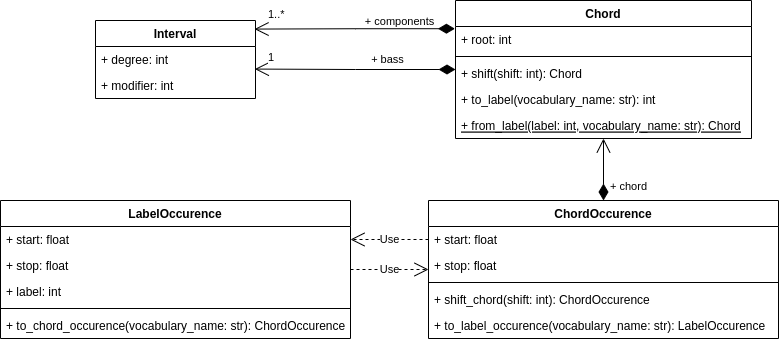
\includegraphics[width=1.0\textwidth]{./images/chord_model.png}
    \caption{Diagram klas UML przedstawiający model obiektowy akordów muzycznych.}
    \label{fig:chord_model}
\end{figure}

\subsection{Parsowanie plików \filetype{lab}}

% wstęp o~formacie lab
Chris Harte w~swojej pracy \cite{harte_towards_nodate}, zanim przedstawił szczegółowo autorski format zapisu akordów, uzasadnił obszernie zapotrzebowanie na tego typu rozwiązanie i~wyliczył podstawowe idee, którymi się kierował. Wykazywał między innymi, że nie istnieje inny, ustandaryzowany między gatunkami i~szkołami, uniwersalny system zapisu akordów.  Wymieniał podstawowe problemy, z~jakimi trzeba się mierzyć, poczynając od niejednoznaczności i~ograniczeń istniejących form zapisu, a~kończąc na problemach związanych z~dużym ryzykiem błędów w~pisowni niektórych symboli.

% opis słowny formatu lab
Zaproponowany przez niego format zapisu akordów odpowiada trzyczęściowej strukturze akordów.  Tekstowa reprezentacja akordu składa się kolejno z~symbolu oznaczającego podstawę, listy interwałów w~postaci skrótu lub dodatkowych interwałów podanych jawnie oraz pojedynczego interwału na końcu oznaczającego bas. Ogólna forma zapisu jest następująca: 
\begin{center}
    \code{root : shorthand (interval1, interval2...) / bass}
\end{center}
W~przeciwieństwie do opisywanej wcześniej struktury danych, w~przypadku zapisu tekstowego, podstawa akordu zapisywana jest w~postaci symbolicznej: jest to nazwa jednego z~7 dźwięków (\code{ABCDEFG}), po której w~razie konieczności następują modyfikatory --- krzyżyki i~bemole, zapisywane odpowiednio jako znaki \code{\#} oraz \code{b}. Fakt, że zamiast litery \code{H} występuje litera \code{B}, która w~naszej notacji oznacza \code{H} obniżone o~pół tonu, wynika z~tego, że w~krajach anglosaskich stosowana jest nieznacznie inna notacja, gdzie litera \code{B} oznacza nasze \code{H}, a~dopiero \code{Bb} oznacza nasze \code{B}. Następnie jest dwukropek, po którym zapisuje się listę interwałów. Może mieć ona postać jawnej listy, poprzedzielanej przecinkami i~ujętej w~nawiasy, gdzie każdy interwał zapisywany jest jako liczba całkowita oznaczająca stopień, w~razie potrzeby poprzedzona krzyżykami lub bemolami. Zamiast podawać listę, można skorzystać z~predefiniowanego skrótu, implikującego odpowiednią listę interwałów. Przykładem takiego skrótu jest \code{min}, oznaczający ciąg interwałów 1, b3 i~5. Można również wykorzystać zarówno skrót, jak i~listę w~nawiasach, dodając w~ten sposób dodatkowe interwały ponad te wynikające ze skrótu, lub usuwając wybrane interwały z~predefinowanej listy, poprzedzając je znakiem \code{*}. Niepodanie listy i żadnego ze skrótów traktuje się jako zwykły akord majorowy (interwały 1, 3~i 5). Na końcu występuje opcjonalny, dodatkowy interwał oznaczający bas, poprzedzony znakiem \code{/}. Jeżeli bas nie jest podany, zakłada się interwał prymy, czyli że podstawa akordu jest jednocześnie jego najniższym dźwiękiem. Zapisany według tej metody akord C-dur wygląda tak:
\begin{center}
    \code{C:(1,3,5)}
\end{center}
lub po prostu tak:
\begin{center}
    \code{C}
\end{center}
Z~kolei akord cis-moll w~pierwszym przewrocie, bez użycia skrótu wygląda tak:
\begin{center}
    \code{C\#:(1,b3,5)/b3}
\end{center}
Wykorzystując skróty, ten sam akord ma postać:
\begin{center}
    \code{C\#:min/b3}
\end{center}
Cały plik \filetype{lab} składa się z~trzech kolumn oddzielonych białymi znakami (np. tabulatorami).  Pierwsza i~druga kolumna zawierają liczby zmiennoprzecinkowe, oznaczające odpowiedni czas rozpoczęcia i~zakończenia trwania akordu w~sekundach. Trzecia kolumna zawiera symbol akordu.

% parsowanie lark'iem - idea, gramatyka, transformer
Aby parsować pliki z~oznaczeniami akordów, wykorzystana została biblioteka \emph{lark}\footnote{\url{https://github.com/lark-parser/lark}}. Biblioteka ta jest zestawem narzędzi, pozwalającym generować parsery do języków bezkontekstowych ang. \emph{context-free language}\footnote{\url{https://en.wikipedia.org/wiki/Context-free_language}}. Język tego typu definiowany jest przez odpowiednią gramatykę bezkontekstową ang. \emph{context-free grammar}\footnote{\url{https://en.wikipedia.org/wiki/Context-free_grammar}}, a~przykładem takiego języka jest praktycznie dowolny język programowania. Również format zapisu akordów stanowi przykład języka bezkontekstowego i~dlatego biblioteka \emph{lark} pozwala bardzo łatwo, w~sposób wydajny i~uporządkowany parsować tego typu oznaczenia. Aby wygenerować instancję parsera, czyli obiektu odpowiedzialnego za proces parsowania, trzeba przygotować opis gramatyki danego języka. Popularnym sposobem opisywania gramatyki bezkontekstowej jest notacja Backusa-Naura (ang. \emph{Backus-Naur form}), której wersję rozszerzoną (ang. \emph{Extended Backu-Naur form})\footnote{\url{https://en.wikipedia.org/wiki/Extended_Backus-Naur_form}} wykorzystuje właśnie biblioteka \emph{lark}. Tak więc przygotowany został plik \url{src/annotation_parser/labfile_grammar.lark}, który zawiera definicję gramatyki formatu \filetype{lab} (jego zawartość prezentowana jest w~tabeli \ref{fig:lab_syntax}). Po sparsowaniu tekstu według podanej gramatyki parser tworzy drzewiastą strukturę, która dzieli ten tekst w~sposób hierarchiczny. Przechodząc przez tę strukturę wiadomo, jaką każdy fragment tekstu odgrywa logiczną rolę (zgodnie z~daną gramatyką) i~jakiej większej konstrukcji jest on częścią. Biblioteka \emph{lark} pozwala przygotować tzw. transformer, czyli obiekt, który jest odpowiedzialny za mapowanie ze wspomnianej struktury drzewiastej (wyniku parsowania) na własną, obiektową strukturę danych. W~pliku \url{src/annotation_parser/labfile_transformer.py} przygotowana została właśnie taka klasa, która pozwala zamienić wynik parsowania pliku \filetype{lab} na instancje klas opisywanego wcześniej modelu obiektowego, a~dokładnie listę obiektów klasy \code{ChordOccurence}. Aby móc przetłumaczyć tekstowe oznaczenia akordów na model obiektowy, potrzebne były mapowania z~symboli literowych reprezentujących dźwięki na wartości całkowite oraz ze skrótów na konkretne zbiory interwałów. Mapy te w~postaci słowników pythonowych zawiera plik \url{src/annotation_parser/labfile_symbols.py}. Kod odpowiedzialny za stworzenie instancji transformera i~parsera oraz opakowanie tego w~funkcję pomocniczą, umieszczony został w~pliku \url{src/annotation_parser/__init__.py}. 

\begin{figure}[tb]
    \centering
    {\scriptsize \verbatiminput{../src/annotation_parser/labfile_grammar.lark}}
    \caption{Opis składni oznaczeń akordów \emph{lab} za pomocą rozszerzonej notacji Backusa-Naura.}
    \label{fig:lab_syntax}
\end{figure}

% tworzenie plików lab
Przygotowana została również możliwość wykonywania operacji odwrotnej do parsowania, czyli wytwarzania plików \filetype{lab} z~modelu obiektowego akordów, który z~kolei może zostać wytworzony z~predykcji sieci. Nie została tutaj wykorzystana żadna specjalistyczna biblioteka --- jedynie podstawowe operacje na ciągach znaków, wraz ze wspomnianymi powyżej mapami symboli skrótów i~symboli dźwięków. Cała logika wytwarzania oznaczeń w~formacie \filetype{lab} zawarta jest w~pliku \url{src/annotation_parser/labfile_printer.py}.

\subsection{Parsowanie plików oznaczeń dla zbioru RS200}

% wstęp o~formacie oznaczeń ze zbioru RS200
Format oznaczeń akordów wykorzystany w~zbiorze RS200 jest znacznie mniej rozbudowany od formatu \filetype{lab}. Jest to jednocześnie format znacznie mniej uniwersalny, nierozwiązujący większości problemów, które format \filetype{lab} rozwiązuje. Nawet dwóch badaczy, którzy równolegle przygotowywali oznaczenia akordów dla zbioru RS200, aby później porównać je między sobą, tak naprawdę nie zachowali spójnej konwencji, mimo iż razem stworzyli ten konkretny format zapisu. Z~tego też powodu, jak już wspomniane przy opisywaniu tego zbioru, dla ułatwienia zadania parsowania, wybrane zostały oznaczenia tylko jednego z~badaczy, który przygotował je w~znacznie prostszy i~bardziej uporządkowany sposób.

% opis słowny formatu oznaczeń ze zbioru RS200
Każde wystąpienie akordu w~utworze charakteryzowane jest przez rodzaj tego akordu i~czas jego wystąpienia. Jeżeli chodzi o~to drugie, to autorzy zdecydowali się na wykorzystanie rekurencyjnej składni (podobnej do notacji Backusa-Naura), wykorzystującej fakt, że utwory dzielą się na pewne logiczne, powtarzalne części. Symbol każdego akordu umieszczony jest w~odpowiedniej części taktu, a~same takty są pogrupowane w~większe struktury, które powtarzają się według określonych wzorców. W~ten sposób, za pomocą zaledwie kilku znaków, można opisać cały utwór. Jest to format jak najbardziej czytelny dla człowieka, ale nie zawierający docelowej informacji, w~której konkretnie sekundzie zaczyna się i~kończy dany akord. Na szczęście autorzy zbioru przygotowali również skrypty, które łączą informacje o~tempie utworu z~oznaczeniami akordów. Skrypty te tworzą nowe pliki z~oznaczeniami (dostępne do pobrania i~wykorzystane w~tej pracy zamiast oryginalnych oznaczeń), które mają format zbliżony do plików \filetype{lab}, gdzie pierwsza kolumna zawiera czas rozpoczęcia danego akordu. Jeżeli chodzi o~symbole akordów, to tutaj również autorzy poszli w~kierunku relatywnego sposobu oznaczania, ponieważ zamiast wykorzystać symbole konkretnych dźwięków, wykorzystują liczby rzymskie oznaczające odległość względem toniki danego utworu.  Symbol każdego akordu składa się najpierw z~liczby rzymskiej, poprzedzonej ewentualnie modyfikatorem --- krzyżykiem lub bemolem. Jeżeli znaki są małe, to oznacza tryb minorowy, jeżeli wielkie, tryb majorowy. Następnie aż do znaku ukośnika mogą występować dowolne symbole, informujące o~modyfikacjach względem zwykłego trójdźwięku majorowego lub minorowego. W~praktyce są to informacje o~występowaniu akordów septymowych, numerach przewrotów oraz akordach, zwiększonych, zmniejszonych i~występowaniu dodatkowych składników jak kwarta. Opcjonalnie, na końcu może wystąpić znak ukośnika i~kolejna liczba rzymska, oznaczająca akordy wtrącone. W~praktyce symbol akordu wykorzystywany jest jedynie do stworzenia listy interwałów i~basu.  Podstawa akordu nie musi być wyliczana na podstawie liczby rzymskiej, ponieważ we wspomnianym powyżej przetworzonym formacie oznaczeń, zawierającym kolumnę z~czasem rozpoczęcia akordu, dodane jest również kolumna z~wartościami całkowitymi, reprezentującymi podstawę akordu względem dźwięku C, a~nie tonacji utworu.

% krótki opis implementacji, bo większość była opisana dla formatu lab
Jeżeli chodzi o~parsowanie plików z~oznaczeniami dla zbioru RS200, to również wykorzystana została biblioteka \emph{lark}. Trzeba więc było przygotować odpowiedni opis gramatyki i~odpowiednią klasę transformującą na model obiektowy. To pierwsze znajduje się w~pliku \url{src/annotation_parser/rs200_dt_grammar.lark}, a~to drugie w~pliku \url{src/annotation_parser/rs200_dt_transformer.py}. Rysunek \ref{fig:rs200_dt_syntax} prezentuje zawartość pliku z~gramatyką. Podobnie jak w~przypadku parsowania formatu \filetype{lab}, plik \url{src/anotation_parser/__init__.py} zawiera kod tworzący instancję parser i~transformera, oraz opakowuje je w~funkcję pomocniczą.

\begin{figure}[tb]
    \centering
    {\scriptsize \verbatiminput{../src/annotation_parser/rs200_dt_grammar.lark}}
    \caption{Opis składni oznaczeń akordów w~zbiorze RS200 za pomocą rozszerzonej notacji Backusa-Naura.}
    \label{fig:rs200_dt_syntax}
\end{figure}


% skrypt evaluation, downloading, 02, 03 i~05 - znalezienie i~pobranie najlepiej pasujących nagrań muzycznych
\section{Pozyskanie plików z~nagraniami muzycznymi pasującymi do oznaczeń}
\sectionmark{Pozyskanie nagrań muzycznych}

% to jest problem generalnie
Znalezienie odpowiednich plików z~nagraniami muzycznymi stanowiło jeden z~głównych problemów, rozwiązywanych w~ramach niniejszej pracy. Jest to problem, z~którym mierzyli się również twórcy poprzednich rozwiązań, ponieważ tak jak wspomniano wcześniej, nieliczne zbiory oznaczeń akordów dostarczane są zazwyczaj bez nagrań muzycznych, ze względu na prawa autorskie muzyków (wyjątkiem jest oczyszczony z~praw autorskich zbiór RWC POP).

\subsection{Analiza koncepcji ręcznego wyszukiwanie nagrań}

% nie można tak po prostu łatwo ich wyszukać - opis i~ocena ręcznej procedury
Pierwszym i~prawdopodobnie prowadzącym do najmniejszej liczby pomyłek sposobem pozyskania utworów muzycznych jest szukanie ,,ręczne''. Polegałoby ono na znalezieniu odpowiednich artystów, albumów i~konkretnych nagrań w~serwisach muzycznych oraz innych ogólnie dostępnych źródłach. W~razie potrzeby wymagałoby to zakupienia odpowiednich nagrań. Każdy zbiór oznaczeń należałoby rozpatrzeć osobno i~w miarę możliwości spróbować pozyskać oryginalne, wykorzystane podczas tworzenia oznaczeń nagrania. W~przypadku zbioru RWC POP nagrania są możliwe do pozyskania za symboliczną opłatą. W~przypadku zbiorów Isohponics, Robbie Williams i~Uspop2002 wiadomo w~miarę dokładnie, o~które nagrania chodzi, ponieważ dla każdego utworu znana jest nazwa albumu. Można próbować dostać się do tych konkretnych albumów, weryfikując wyrywkowo, czy w~znalezionych albumach oznaczenia pasują do nagrań. Możliwe jest jednak, że trafi się na jakieś poprawione wydania, gdzie wszystkie utwory będą np. przesunięte w~czasie. Można wtedy próbować je ,,naprawić'' za pomocą odpowiedniego programu komputerowego. Co do pozostałych zbiorów, to nie jest znany album i~w tym przypadku zdecydowanie już nie można łatwo stwierdzić, które spośród wielu możliwych nagrań będzie pasowało do oznaczeń. Trzeba by więc samodzielnie odsłuchać fragment każdej znalezionej wersji nagrania i~znaleźć tą odpowiednią, w~najgorszym przypadku odrzucając wszystkie i~pozostając z~samymi oznaczeniami akordów. Tak więc metoda ta, chociaż najdokładniejsza, jest niezwykle czasochłonna i~trudno skalowalna w~przypadku znalezienia większej liczby oznaczeń. Co więcej, i~tak nie daje ona pewności, że nie trafią się nagrania niepasujące, chyba że ostatecznie każde wybrane nagranie zostanie przesłuchane i~porównane z~oznaczeniami akordów. Warto zaznaczyć, że cały opis powyższej procedury ,,ręcznej'', choć przemyślany, jest jedynie teoretyczny (nie był zrealizowany od początku do końca) i~nie wiadomo, jakie problemy okazałyby się mało znaczące, a~jakie nie zostały wzięte pod uwagę. 

\subsection{Motywacja i~decyzja o~automatycznym wyszukiwaniu nagrań}

% motywacja i~decyzja o~procedurze automatycznej
W~ramach niniejszej pracy zdecydowano się na automatyczną procedurę wyszukiwania odpowiednich utworów muzycznych w~serwisie YouTube Music\footnote{music.youtube.com}. Takie podejście prowadzi prawdopodobnie do pozyskania większej ilości niepasujących nagrań i~co ważniejsze, w~ogóle do pozyskania mniejszej ilości nagrań. Jest to jednak podejście zdecydowanie szybsze. Automatyzacja procesu wyszukiwania odpowiednich nagrań sama w~sobie stanowi ciekawy problem, którego możliwe rozwiązania wydają się cenne, ze względu na swoją szybkość, powtarzalność i~skalowalność.  Ponadto rozwiązuje częściowo problem reprodukcji i~kontynuacji badań przez inne osoby.  Przygotowane w~ramach niniejszej pracy skrypty można by umieścić w Internecie, ułatwiając zadanie innym osobom zajmującym się tym samym tematem. Nie można natomiast rozpowszechniać w~ten sposób nagrań muzycznych. Z~tych powodów zdecydowano się, że ostatecznie zbiór danych oznaczonych będzie prawdopodobnie trochę mniejszy i~bardziej zanieczyszczony, niż w~przypadku ręcznego wyszukiwania odpowiednich utworów. Poświęcono natomiast czas na przygotowanie nieskomplikowanego algorytmu, opierającego się na kilku prostych założeniach, pozwalającego automatycznie wyszukiwać odpowiednie nagrania w~serwisie YouTube Music. Algorytm ten można opisać w~kilku prostych krokach. Wśród nich występują jednak trzy bardziej złożone operacje: wyszukiwanie utworu w~serwisie YouTube Music, pobieranie konkretnego nagrania na dysk lokalny oraz ewaluacja tego nagrania --- oceny jak dalece jest ono zgodne z~dostępnymi oznaczeniami akordów. Wszystkie trzy operacje są szczegółowo opisane poniżej.

\subsection{Wyszukiwanie utworów w~serwisie YouTube Music}

% opis wyszukiwania utworów i~liba ytmusicapi
Wyszukiwanie utworów w~serwisie YouTube Music zostało wykonane za pomocą nieoficjalnego klienta pythonowego do tego serwisu --- \emph{ytmusicapi}\footnote{\url{https://github.com/sigma67/ytmusicapi}}.  Daje on mniej więcej takie same możliwości jak korzystanie z~oficjalnego, graficznego klienta przeglądarkowego. Można jednak wszystkie operacje łatwo zautomatyzować. Jest to przykład tak zwanego \emph{web scrappingu}, który w~tym przypadku jest niezbędny, jako że oficjalne API do tego konkretnego serwisu nie istnieje, a~dostępne w~ograniczonym zakresie (ograniczona liczba zapytań) API do całego serwisu YouTube nie daje wystarczających możliwości przeszukiwania dostępnych tam nagrań muzycznych.  Korzystanie z~klienta \emph{ytmusicapi} jest niezwykle proste. Trzeba jedynie stworzyć instancję obiektu \code{YTMusic} (jest to dostęp analogiczny jak dla niezalogawnego użytkownika w~przeglądarce) i~wywołać metodę \code{search} przyjmującą tekstowe zapytanie (takie jak wpisywane w~pole wyszukiwania w~kliencie graficznym) oraz filtr, ograniczający wyniki do danego typu treści, np.  tylko do nagrań muzycznych, lub tylko do filmów. W~zwróconych wynikach dostępne są informacje o~identyfikatorze zasobu (\code{video\_id}), tytule utworu, artyście (lub artystach) i~albumie (jeżeli dotyczy).

\subsection{Pobieranie nagrań z~serwisu YouTube na dysk lokalny}

% opis pobierania utworów - skryptu i~liba pytube
Pobieranie nagrań na dysk lokalny również jest zrealizowane za pomocą nieoficjalnego, pythonowego klienta, tym razem już do całego serwisu YouTube --- \emph{pytube}\footnote{\url{https://github.com/pytube/pytube}}. Służy on właściwie nie tyle do przeszukiwania serwisu YouTube, ile do pobierania z~niego całych filmów lub samych ścieżek dźwiękowych w~dostępnych formatach i~jakościach. Aby z~niego skorzystać, trzeba stworzyć instancję klasy \code{YouTube}, podając jako argument adres URL konkretnego filmu, przy czym wystarczy oczywiście znać jedynie jego \code{video\_id} (\url{http://youtube.com/watch?v=\emph{video_id}}). Następnie można filtrować dostępne formaty i~ostatecznie pobrać wybrany strumień na dysk. Przygotowana została funkcja pomocnicza (\url{src/dataset_scripts/downloading.py}), która dla danego \code{video\_id}, jeżeli nagranie nie zostało jeszcze pobrane (nie istnieje plik we wskazanym katalogu), wybiera pośród dostępnych strumieni z~samym dźwiękiem ten w~najlepszej jakości i~zapisuje go jako plik dźwiękowy do wskazego katalogu. Pobieranie to może się z~różnych powodów nie powieść (błąd sieci, YouTube odrzuca podejrzane żądanie, etc.).

\subsection{Ewaluacja nagrań --- ocena dopasowania do oznaczeń akordów}

% opis idei ewaluacji nagrań i~liba madmom
Ewaluacja nagrań jest najbardziej skomplikowaną i~jednocześnie najważniejszą częścią całego procesu wyszukiwania nagrań. Aby automatycznie ocenić, czy nagranie pasuje do oznaczeń, trzeba automatycznie rozpoznać jakie akordy w~nim występują. Z~kolei przygotowanie algorytmu rozpoznającego akordy stanowi jeden z~podstawowych celów niniejszej pracy. Oczywiście nie można się więc na tym etapie posłużyć własnym rozwiązaniem. Istnieje natomiast dużo gotowych, wysokopoziomowych bibliotek, które realizują to zadanie, z~większą bądź mniejszą dokładnością. Wysoka dokładność takiego algorytmu nie ma na tym etapie dużego znaczenia, chodzi jedynie, aby poglądowo ocenić, czy dane nagranie pasuje do oznaczeń, czy może jest to zupełnie inny utwór, czy jedynie inna, wolniejsza lub trochę przesunięta w~czasie wersja oryginalnego nagrania. Zdecydowano się na użycie biblioteki \emph{madmom}\footnote{\url{https://github.com/CPJKU/madmom}}.  Biblioteka ta, podobnie jak dwie poprzednie i~w ogóle zdecydowana większość bibliotek języka Python, jest bardzo prosta w~użyciu. Trzeba wybrać odpowiedni algorytm, stworzyć jego instancję i~wywołać przekazując ścieżkę do pliku. Pod spodem wykorzystywana jest biblioteka \emph{ffmpeg} do odczytania praktycznie dowolnego formatu. Za pomocą wytrenowanego wcześniej modelu rozpoznawane są występujące akordy (standardowe 25 klas) i~zwracane są czasy ich występowania oraz symbole w~formacie wykorzystywanym w~plikach \filetype{lab} (zgodnym z \cite{harte_towards_nodate}). Ze względu na niewielkie wymagania dotyczące jakości klasyfikacji i~większe wymagania dotyczące szybkości działania, zdecydowano się użyć prostszego z~dwóch dostępnych algorytmów, czyli \emph{Deep Chroma Extractor} \cite{korzeniowski_feature_2016}.

% dokładny opis procedury ewaluacji (skryptu ewaluacyjnego)
Cała procedura ewaluacji nie kończy się na wywołaniu biblioteki i~rozpoznaniu występujących akordów.  Trzeba wybrać odpowiednie metryki pozwalające łatwo porównać między sobą kilka dostępnych nagrań dla tego samego zestawu oznaczeń akordów. Po pierwsze wykorzystana została podstawowa miara CSR. Po drugie dla każdego nagrania liczone jest przesunięcie czasowe pomiędzy początkiem pierwszego oczekiwanego (z pliku z~oznaczeniami) i~pierwszego rozpoznanego (za pomocą biblioteki \emph{madmom}) akordu (\code{start\_diff}) oraz przesunięcie czasowe pomiędzy końcem ostatniego oczekiwanego i~ostatniego rozpoznanego akordu (\code{stop\_diff}). Oczywiście poprzez wystąpienie akordu rozumie się wystąpienie akordu dowolnej klasy poza klasą 0 (brak akordu). Realizująca wszystkie te operacje funkcja pomocnicza znajduje się w~pliku \url{src/dataset_scripts/evaluation.py}. W~przypadku, gdy żaden akord nie występuje w~oznaczeniach lub nie został rozpoznany, funkcja ta nie zwraca żadnych wartości.

% interpretacja metryk
Metryka CSR pozwala ocenić, w jakim stopniu znalezione akordy są zgodne z~oczekiwanymi. Metryki prezentujące przesunięcie czasowe dodatkowo pozwalają wykryć sytuację, kiedy znalezione nagranie zaczyna się w~innym momencie albo jest zdecydowanie za długie. W~obu tych sytuacjach wciąż możliwa jest względnie wysoka wartość miary CSR. W~konsekwencji miara ta nie pozwala łatwo wyeliminować nagrań, które z~powodu różnej długości z~całą pewnością nie pasują do oznaczeń.

\subsection{Algorytm automatycznego wyszukiwania pasujących nagrań muzycznych}

% opis całego algorytmu ze skryptu 02
Poniższe kroki są wykonywane dla każdej pozycji z~indeksu (\url{data/index.csv}) opisującego cały dostępny zbiór oznaczeń. Przechodzenie przez cały indeks dzieje się równolegle w~16 procesach, jako że w~zastosowanym algorytmie nie ma żadnych zależności między poszczególnymi utworami. Wynikiem działania algorytmu są dodatkowe kolumny w~pliku \url{index.csv}, prezentujące identyfikator najlepszego znalezionego nagrania (\code{video\_id}) oraz wyniki ewaluacji tego nagrania: przesunięcie początku pierwszego akordu (\code{start\_diff}) i~zakończenia ostatniego (\code{stop\_diff}) względem pliku z~oznaczeniami oraz wartość miary CSR (\code{csr}).

Poniższy algorytm jest dodatkowo przygotowany w~taki sposób, aby móc wykonywać go wielokrotnie dla tego samego indeksu w~celu wyszukiwania nagrań dla nowo dodanych plików z~oznaczeniami, skorzystania z~dostępnych od niedawna nagrań lub po prostu kontynuacji przerwanego działania, które jest czasochłonne i~może zostać przerwane z~powodu różnych błędów.

Kroki algorytmu są następujące:
\begin{enumerate}
    \item Jeżeli dany utwór ma już dopasowane nagranie (\code{video\_id}) i~jest ono zewaluowane, to
        zakończ działanie.
    \item Jeżeli dany utwór ma już dopasowane \code{video\_id} i~NIE jest ono zewaluowane, to zrób
        ewaluację tego nagrania i~zakończ działanie.
    \item Wyszukaj nagrania w~serwisie YouTube Music zapytaniem ,,tytuł artysta album (jeśli jest
        znany) ''. Filtr ustawiony na nagrania muzyczne. Ogranicz do 10 wyników.
    \item Pierwszy etap selekcji --- na podstawie nazw. Etap ten ma na celu zmniejszyć liczbę
        czasochłonnych ewaluacji z~etapu drugiego. 
        \begin{enumerate}
            \item Znormalizuj nazwy albumu, utworu i~artystów dla danego utworu i~we wszystkich
                wynikach wyszukiwania poprzez zamianę wielkich liter na małe i~pozostawienie tylko
                znaków alfanumerycznych oraz znaku ,,\_''.
            \item Wybierz te wyniki wyszukiwania, dla których nazwy albumu (jeśli jest
                dostępna), utworu i~artystów zawierają w~sobie odpowiednie nazwy z~indeksu.
            \item Jeżeli żadne nagranie nie pasuje na tym etapie, wszystkie przechodzą dalej.
        \end{enumerate}
    \item Drugi etap selekcji --- na podstawie ewaluacji.
        \begin{enumerate}
            \item Pobierz na dysk nagrania z~pozostałych po etapie pierwszym wyników wyszukiwania
            \item Dokonaj ewaluacji każdego z~pobranych nagrań i~zapamiętaj wartości metryk
            \item Usuń nagrania z~dysku
            \item Wybierz to nagranie, które ma najwyższą wartość WCSR i~zapisz w~indeksie jego
                \code{video\_id} oraz wartości metryk z~ewaluacji
        \end{enumerate}
\end{enumerate}

\subsection{Selekcja i~podział utworów, dla których znaleziono dobre nagranie}

% opis skryptu 03 - selekcja i~podział na foldy
Na tym etapie indeks opisujący wszystkie dostępne pliki z~oznaczeniami był rozszerzony o~kolumny zawierające informacje o~identyfikatorze nagrania z~YouTube oraz o~metrykach z~ewaluacji tego nagrania. Chociaż prawie dla każdego pliku z~oznaczeniami znalezione zostało jakieś \code{video\_id}, to w~wielu przypadkach nagranie to zupełnie nie pasowało do oznaczeń. Trzeba było ustalić pewną granicę decyzyjną, opartą o~wartości metryk, według której nagrania zostaną uznane za pasujące do plików z~oznaczeniami. Znalezienie takiej granicy nie było trywialne. Należało wybrać losowo niewielką część nagrań ze zróżnicowanymi wynikami ewaluacji, odsłuchać fragmenty tych nagrań i~ocenić, co w~praktyce oznaczają takie, a~nie inne wartości metryk. Głównie chodziło o~to, aby stwierdzić, jakie są możliwe przyczyny słabych wyników ewaluacji, z~czego wynikają przesunięcia w~początku i~zakończeniu utworu oraz czy zawsze implikują one niepasujące nagranie. Praca ta była chaotyczna i~nie została udokumentowana w żaden specjalny sposób. Jedynym jej wynikiem jest zdecydowanie się na wykorzystanie tylko tych nagrań, dla których wartość CSR była większa niż $0.3$, a~wartość bezwzględna przesunięcia końca utworu mniejsza niż $10$ sekund. Warunek ten prezentuje poniższe równanie:
\begin{center}
    \code{CSR > $0.3$ AND |stop\_diff| < $10$}
\end{center}
Oczywiście granica ta jest bardzo umowna --- nie ma żadnej pewności, że wśród wykorzystanych nagrań nie ma nagrań błędnych, jak i że wśród nagrań usuniętych, nie ma nagrań poprawnych. Nie udało się niestety znaleźć innej metody ewaluacji i~ostatecznie trzeba było zdecydować się na jakąś wartość progową, wiedząc, że opiera się ona po części na intuicji, a~po części na ślepym losie.

Operację odfiltrowania ,,niepasujących'' nagrań zaimplementowano w~skrypcie \url{src/dataset_scripts/03-select_proposals_and_split.py}. Po wykonaniu progowania z $1268$ utworów pozostało jedynie $995$. Następnie usuwane są również te utwory, które mają dopasowane to samo nagranie co inny utwór. Znalazł się tylko $1$ taki przypadek. Tak więc ostatecznie pozyskano ,,pasujące'' nagrania dla $994$ utworów. W~ramach tego samego skryptu wszystkie te utwory zostały losowo podzielona na 5~części (ang. \emph{folds}) do późniejszej walidacji krzyżowej. Równy podział na $5$ zachowany został w~ramach każdego zbioru oznaczeń. Podział ten został zapisany w~nowej kolumnie \code{purpose} w~pliku \url{data/index.csv} (wartości \code{train\_fold\_0}, \code{train\_fold\_1} itd.). Wpis w~tej kolumnie jest jednocześnie znacznikiem, że dla danego pliku z~oznaczeniami znaleziono pasujące nagranie i~może być on wykorzystany do treningów.

\subsection{Pobieranie utworów i~podsumowanie ich liczebności}

Ostatnim etapem jest ponowne pobranie wszystkich nagrań z~serwisu YouTube. Operacja ta została wydzielona do osobnego kroku i~osobnego skryptu, ponieważ nagrania te zajmują względnie dużo miejsca i~nie powinny być rozpowszechniane. Dzięki temu nie muszą być więc przechowywane, a~mogą być z łatwością od nowa pobrane z~serwisu YouTube, kiedy projekt jest klonowany lub przenoszony na inną maszynę. Mając więc gotowy plik indeksu, stanowiący stałą część repozytorium projektu, należy wywołać skrypt \url{src/dataset_scripts/05-download_songs.py}, który pobiera wszystkie nagrania z~pliku indeksu, dla których istnieje wartość w~kolumnie \code{purpose}. Pobiera je, wykorzystując opisaną wcześniej funkcję pomocniczą z~pliku \url{src/dataset_scripts/downloading.py}, czyli wybierając najlepszy dostępny strumień dźwiękowy i~zapisując go w~postaci pliku dźwiękowego, w~katalogu \url{data/audio}. Dodatkowo do pliku indeksu dodawana jest nowa kolumna \code{audio\_filepath}, która dla każdego pobranego utworu zapisuje ścieżkę do pliku dźwiękowego.

Tab. \ref{tab:datasets2} prezentuje rozkład 994 pobranych i~wykorzystywanych do eksperymentów nagrań, pomiędzy poszczególne zbiory danych z~oznaczeniami. Tab. \ref{tab:datasets3} prezentuje natomiast liczebność nagrań we wszystkich 5~częściach do walidacji krzyżowej. Ponieważ liczba utworów nie jest podzielna przez $5$, to jedna część jest nieznacznie większa od pozostałych.  Wszystkie nagrania pobierane są w najlepszej dostępnej jakości. Prawie wszystkie pliki (z wyjątkiem dwóch) zostały pobrane w~formacie \filetype{webm}, z~częstotliwością próbkowania $48000$ Hz i $32$-bitową dokładnością zapisu. Pozostałe dwa nagrania pobrane zostały w~formacie \filetype{mp4} z~częstotliwością próbkowania $44100$ i~tą samą dokładnością zapisu.

Jak widać w~Tab. \ref{tab:datasets2}, nie udało się znaleźć żadnego pasującego nagrania do oznaczeń ze zbioru RWC POP. Jest to spowodowane faktem, że większość utworów w~tym zbiorze to japońska muzyka popularna, która nie jest dostępna, lub nie udało się jej wyszukać zastosowaną metodą w~serwisie YouTube Music. Sytuacja ta jest jednak zupełnie akceptowalna i~zrozumiała w~kontekście próby stworzenia całkowicie automatycznego algorytmu wyszukiwania odpowiednich nagrań w~Internecie.

\begin{table}
    \centering
    \caption{Liczebności pobranych i~wykorzystywanych do eksperymentów nagrań między poszczególnymi zbiorami danych z~oznaczeniami.}
    \label{tab:datasets2}
    \begin{tabular}{|l|c|c|}
        \hline
        Nazwa zbioru & Liczba nagrań & Łączny czas trwania [h] \\
        \hline
        Isophonics          & $217$ & $10.5$ \\ % Loaded 217 songs (10:18:27)
        McGill Billboard    & $420$ & $24.5$ \\ % Loaded 420 songs (1 day, 0:34:52)
        Robbie Williams     & $54$  & $4$    \\ % Loaded 54 songs  (4:10:22)
        RS200               & $142$ & $8.5$  \\ % Loaded 142 songs (8:43:31)
        RWC POP             & $0$   & $0$    \\
        Uspop2002           & $161$ & $11.5$ \\ % Loaded 161 songs (11:19:29)
        \hline
        SUMA                & $994$ & $59$   \\
        \hline
    \end{tabular}
\end{table}

\begin{table}
    \centering
    \caption{Liczności poszczególnych części zbioru, wykorzystywanych do walidacji krzyżowej.}
    \label{tab:datasets3}
    \begin{tabular}{|l|c|c|}
        \hline
        Numer części & Liczba nagrań \\
        \hline
        1  & 197 \\
        2  & 197 \\
        3  & 197 \\
        4  & 197 \\
        5  & 206 \\
        \hline
    \end{tabular}
\end{table}

Mając już wybrane, które konkretnie utwory będą wykorzystywane do eksperymentów, można było zbadać rozkład częstości występowania poszczególnych typów akordów w~tych utworach. Rysunek \ref{fig:chords_histogram} prezentuje, ile godzin zajął sumarycznie każdy z $25$ rozpoznawanych typów akordów.

\begin{figure}
    \centering
    \makebox[\textwidth][c]{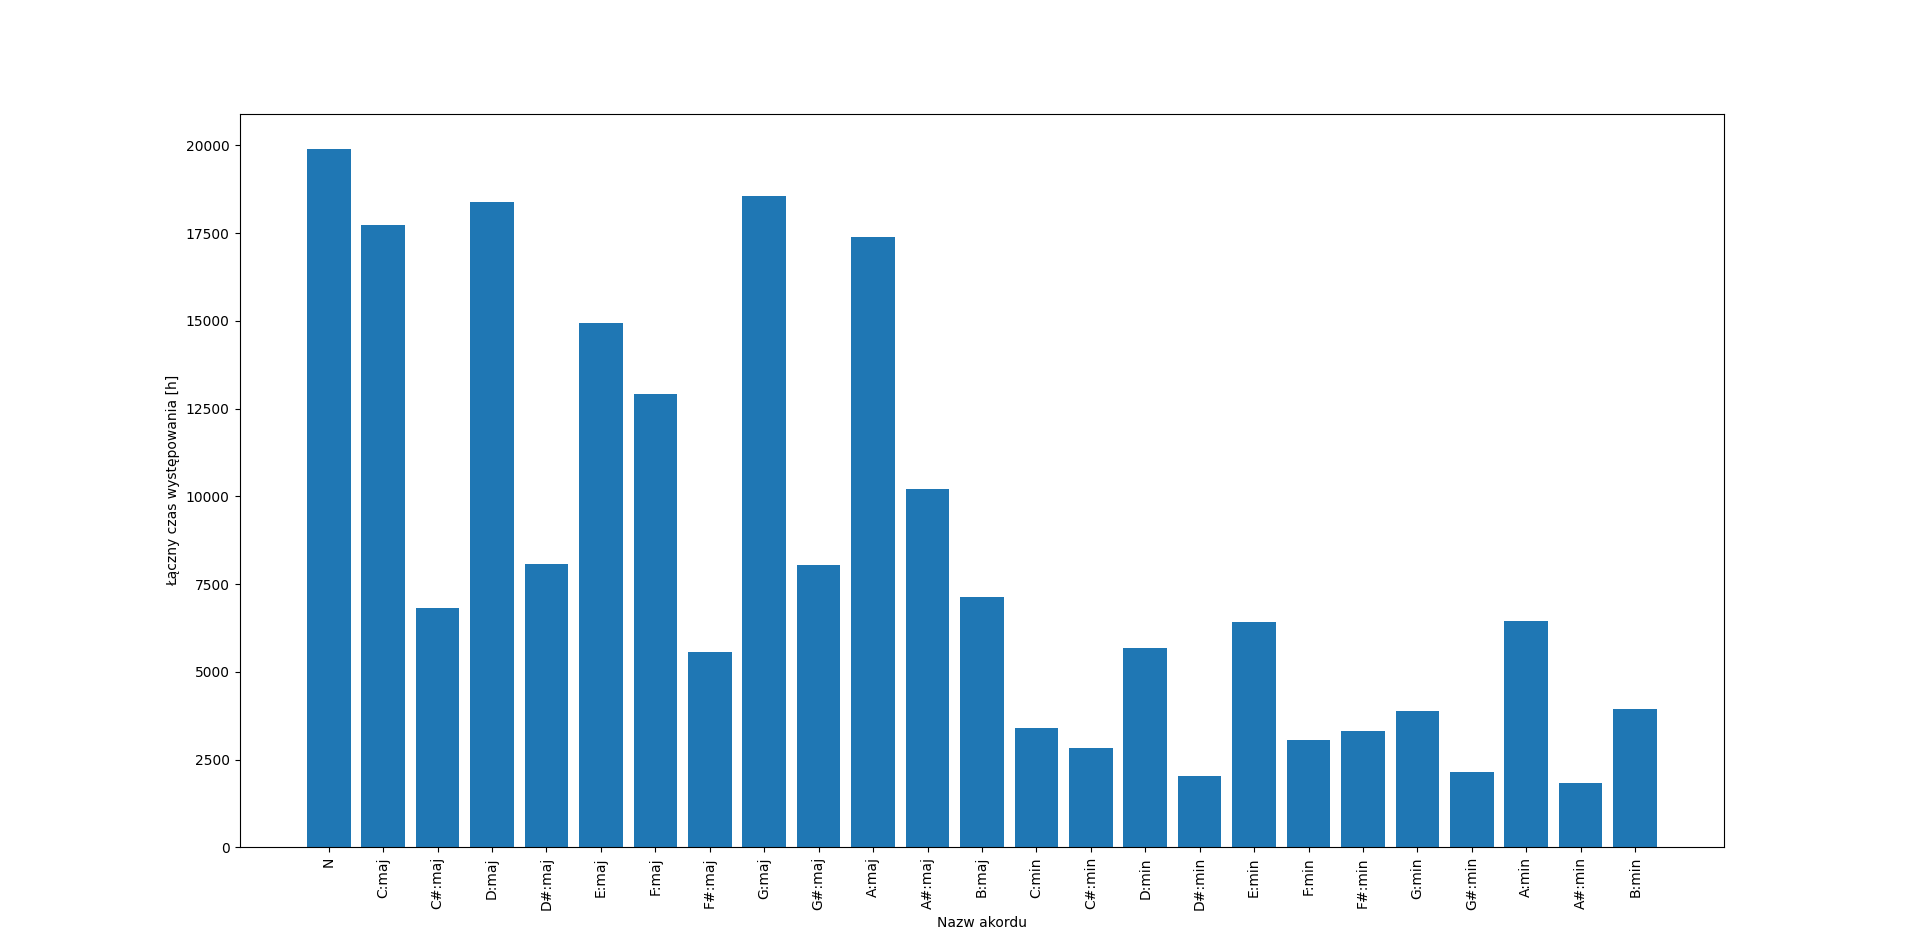
\includegraphics[width=1.5\textwidth]{./images/chords_histogram.png}}
    \caption{Rozkład występowania każdej z $25$ klas akordów w $994$ utworach wykorzystywanych w~eksperymentach. Klasa \code{N} oznacza takie fragmenty, których nie udało się przyporządkować do żadnej z~pozostałych $24$ klas akordów (jak opisano w~rozdziale \ref{subsection:chord_model}).}
    \label{fig:chords_histogram}
\end{figure}


\section{Wyszukiwanie utworów bez oznaczeń z~rankingów magazynu Billboard}
\sectionmark{Wyszukiwanie utworów bez oznaczeń}

% TODO: statystyki o~zbiorze nieoznaczonym
% wstęp
Jak już wspomniano wcześniej, zgromadzenie zbioru danych nieoznaczonych było znacznie prostsze. Dla przypomnienia chodzi tutaj jedynie o~same nagrania muzyczne, bez oznaczeń akordów. W~najprostszym rozumieniu wystarczyłoby więc pobrać dowolną liczbę dowolnych nagrań muzycznych z~Internetu i~zadanie będzie wykonane. Trzeba natomiast zorganizować ten proces w~taki sposób, aby nagrania te się nie powtarzały i~aby, co ważniejsze, stanowiły pewną reprezentatywną próbę dla muzyki danego gatunku, w~tym przypadku dla popularnej muzyki zachodniej (ang. \emph{Western Music}). Trzeba więc uniknąć sytuacji, kiedy zbyt wiele nagrań będzie pochodziło z~tego samego okresu, z~tego samego specyficznego nurtu, lub nawet od tego samego artysty. W~ramach niniejszej pracy zdecydowano się na bardzo proste podejście do tematu wyboru tychże utworów --- były one losowo wybierane (bez powtórzeń) ze wszystkich dostępnych rankingów \emph{Hot 100} magazynu \emph{Billboard}. Jest to więc metoda niejako skopiowana od twórców zbioru McGill Billboard. Zapewnia ona, że wybrane utwory będą z~różnych okresów, od różnych artystów i~w różnych stylach. Będą również, ze względu na swoją wysoką popularność, stanowiły reprezentatywną grupę muzyki popularnej zachodu. Znalezione w~ten sposób utwory były następnie wyszukiwane w~serwisie YouTube Music i~w razie dostępności pobierane i~dodawane do pliku indeksu. Wyszukanych i~pobranych tą metodą zostało 10000 różnych nagrań.

Cały algorytm automatycznego przeszukiwania rankingów magazynu \emph{Billboard} oraz serwisu YouTube Music został zaimplementowany w~skrypcie \url{src/dataset_scripts/04-collect_big_dataset.py}. Jest to implementacja umożliwiająca przeszukiwanie w~wielu wątkach jednocześnie (w ramach pracy wykorzystanych zostało 5~wątków), ze względu na to, że krytycznymi pod względem czasu operacjami są zapytania do Internetu, a~cała procedura jest czasochłonna. Algorytm ten składa się z~dwóch zasadniczych części: pierwsza związana jest z~przeszukiwaniem rankingów \emph{Hot 100} a~druga z~wyszukiwaniem kandydujących utworów w~serwisie YouTube Music.

Pierwsza z~dwóch części algorytmu została zaimplementowana w~postaci pythonowego generatora o~nazwie \code{billboard\_hot100\_item\_generator}. Generator ten zaczyna od stworzenia listy dat wszystkich niedziel od 9~kwietnia 1958 roku, kiedy to dostępny jest najstarszy, cotygodniowy ranking \emph{Hot 100} magazynu \emph{Billboard}. Ranking ten prezentuje najpopularniejsze w~danym tygodniu utwory z~różnych gatunków muzycznych, mierzone według aktywności serwisów streamingowych. Każda data z~powstałej listy odpowiada zatem jednemu rankingowi, ze wszystkich dostępnych, od najstarszego aż dotąd. Zwracając kolejne wyniki, generator iteruje przez te wszystkie daty w~losowej kolejności.  Dla każdej z~nich wykonuje zapytanie do serwisu internetowego magazynu \emph{Billboard}\footnote{\url{https://www.billboard.com/charts}}, wykorzystując w~tym celu dedykowaną, pythonową bibliotekę \emph{billboard.py}\footnote{\url{https://github.com/guoguo12/billboard-charts}}.  Zapytanie to zwraca dla danej daty listę tytułów utworów, wraz z~nazwiskami artystów (album nie jest znany). Przechodząc przez kolejne rankingi, generator zapisuje i~sprawdza, czy znalezione utwory nie były już wcześniej zwrócone, ponieważ często się zdarza, że ten sam utwór występuje na wielu rankingach. Podsumowując, generator ten dostarcza losowe pozycje z~rankingów \emph{Hot 100} magazynu \emph{Billboard} w~postaci jednej, bardzo długiej, niezawierającej powtórzeń, generowanej dynamicznie listy.

Drugą część implementacji stanowi uruchamiana w~wielu wątkach jednocześnie funkcja \code{find\_next\_hot\_song}. Zadaniem tej funkcji jest pobrać kolejną parę tytuł-nazwisko z~opisywanego powyżej generatora i~wyszukać ją w~serwisie YouTube Music. Wyszukiwanie przebiega z~pomocą opisywanej wcześniej biblioteki \emph{ytmusicapi}. Wyniki wyszukiwania są ograniczone do utworów muzycznych. Spośród pierwszych trzech wyników brany jest pierwszy taki, którego \code{video\_id} nie zostało już pobrane dla jakiegoś innego utworu. Jeżeli znajdzie się takie nagranie, to jest ono pobierane na dysk (za pomocą opisywanego wcześniej skryptu pomocniczego z~pliku i~biblioteki \emph{pytube}) i~dodawane do pliku indeksu. Wszystkie znalezione w~ten sposób nagrania mają specjalną wartość \code{,,pretrain''} w~kolumnie \code{purpose}. Oczywiście wiersze indeksu związane z~tymi nagraniami nie mają zapisanej ścieżki do pliku z~oznaczeniami.

W~przypadku wyszukiwania dużej liczby utworów za pomocą tego algorytmu, może dojść do sytuacji, że znalezione nagrania będą się powtarzać, nie będą związane z~danym utworem lub, że w~ogóle nie uda się znaleźć nagrania dla danego zapytania. Wszystkie te przypadki zostały rozważone i~ze względu na naturę tego wyszukiwania nie są problematyczne. Algorytm został napisany tak, aby wszystkie wyniki były unikalne. Jeżeli nie uda się znaleźć unikalnego nagrania, po prostu algorytm przechodzi do kolejnej, losowej pozycji z~rankingów \emph{Billboard}, aż nie zwróci zadanej liczby różnych nagrań z~serwisu YouTube Music. Nagrania niepasujące do wyszukiwanych tytułów utworów również nie są problematyczne, ponieważ wykorzystanie tutaj tych, a~nie innych tytułów jest jedynie pewnym punktem wyjścia do zgromadzenia dużej liczby różnorodnych, popularnych nagrań. Pojedyncze przypadki nagrań spoza tej konkretnej listy nie stanowią najmniejszego problemu, są nawet pożądane, ze względu na różnorodność zbioru.

\section{Wstępne przetwarzanie danych} \label{sec:preprocessing}

% TODO: dodać jakiś ładny schemat prezentujący cały preprocessing (obrazki spektrogramów itd.)
% wstęp
W~poprzednich podrozdziałach opisany został proces gromadzenia plików z~oznaczeniami, gromadzenia plików z~nagraniami i~utworzenia indeksu, opisującego cały powstały zbiór danych. Ostatnim etapem prac, związanym z~przygotowaniem danych, jest przedstawienie ich w~formie nadającej się na wejście sieci neuronowej. Całe to \emph{wstępne przetwarzanie danych} (ang. \emph{preprocessing}) zostało przygotowane na podstawie \cite{park_bi-directional_2019}, ponieważ to właśnie ta praca stanowi główny punkt odniesienia dla otrzymanych wyników. Wszystkie opisane poniżej kroki przetwarzania zgromadzonych danych, zostały zaimplementowane w~postaci klasy \code{Dataset} biblioteki PyTorch, w~pliku \url{src/training/dataset.py}.

\subsection{Wstępne przetwarzanie plików dźwiękowych}

\subsubsection{Wczytywanie plików}

% format zapisu dźwięku
W~swojej surowej, nieskompresowanej postaci, plik dźwiękowy ma postać długiego ciągu, lub kilku ciągów próbek. Każdy taki ciąg (tzw. kanał), reprezentuje inną część nagrania (np. inny instrument, inne źródło nagrywania). Próbki z~kolei są po prostu liczbami rzeczywistymi, reprezentującymi w~sposób dyskretny falę dźwiękową (jej stan w~kolejnych chwilach czasu). Taka cyfrowa reprezentacja sygnału dźwiękowego pozwala odtworzyć nagranie za pomocą odpowiedniego sprzętu lub wykonać najróżniejsze analizy, w~tym również rozpoznawanie akordów.

% wczytywanie surowych danych
Aby wczytać zapisane na dysku pliki dźwiękowe do programu pythonowego w~opisanym powyżej, surowym formacie, wykorzystana została popularna biblioteka \emph{librosa} \cite{mcfee_librosa_2015}. Ma ona bardzo prosty i~przejrzysty interfejs. Między innymi dostarcza funkcję \code{load}, która przyjmuje ścieżkę do pliku i~zestaw parametrów, na podstawie których wczytuje nagranie z~dysku, jeśli trzeba resampluje i~zwraca w~formie tablicy próbek. Wykorzystane parametry ładowania nagrań za pomocą tej funkcji zostały wymienione w~Tab. \ref{tab:load_audio_params}. Na ogół podczas ładowania, niezależnie od formatu pobranych z~serwisu YouTube plików wejściowych, wszystkie nagrania są resamplowane do częstotliwości $22050$ Hz, a~wszystkie kanały są miksowane do jednego.

\begin{table}
    \centering
    \caption{Parametry ładowania nagrań muzycznych za pomocą bibiloteki \emph{librosa}.}
    \label{tab:load_audio_params}
    \begin{tabular}{|l|l|} \hline
        Docelowa liczba kanałów & 1 \\ \hline
        Docelowa częstotliwość próbkowania & $22050$Hz \\ \hline
        Algorytm resamplingu & \code{kaiser\_fast} \\ \hline
    \end{tabular}
\end{table}

\subsubsection{Tworzenie spektrogramów}

% uzasadnienie wykorzystania spektrogramów
Istnieją modele, dla których gotowym formatem wejściowym jest jedynie zresamplowany do odpowiedniej częstotliwości surowy sygnał dźwiękowy \cite{baevski_wav2vec_2020}. Jednakże, w~zadaniu rozpoznawania akordów, praktycznie zawsze stosuje się dodatkowy etap wstępnego przetwarzania sygnału dźwiękowego: przejście w~dziedzinę częstotliwości, czyli stworzenie spektrogramu. Może mieć on różne formy, ale zazwyczaj bazuje na dyskretnej transformacji Fouriera. Ta dwuwymiarowa reprezentacja dźwięku była szczególnie korzystna w~przypadku klasycznych metod rozpoznawania akordów. Spowodowane jest to tym, że bezpośrednio zawiera informacje o~wysokościach poszczególnych dźwięków składowych, jest więc łatwa w~interpretacji i~czytelna dla człowieka. W~przypadku modeli, jakimi są sieci neuronowe, reprezentacja ta nie jest już tak krytyczna, sieć może bowiem względnie łatwo sama nauczyć się najlepszej transformacji dla danego zadania. Ponieważ jednak spektrogramy są wciąż powszechnie wykorzystywane w~obszarze MIR, w~ramach tej pracy również wykorzystana została ta reprezentacja. 

% metoda i~parametry tworzenia spektrogramów
Do utworzenia spektrogramów również została wykorzystana biblioteka \emph{librosa}, a~dokładnie funkcja \code{cqt}. Jak wynika z~nazwy tej funkcji, w~ramach niniejszej pracy utwory były prezentowane za pomocą spektrogramów na bazie \emph{Constant-Q Transform}. Ponieważ wynik tej transformacji ma postać zespoloną, z~surowych spektrogramów wyliczana jest wartość bezwzględna, która jest jeszcze dodatkowo logarytmowana. Szczegółowe wartości parametrów wykorzystanych do stworzenia spektrogramów prezentowane są w~Tab. \ref{tab:spectrogram_params}. Nagrania są więc dzielone na ramki, z~częstotliwością około $11$ ramek na sekundę. Każda z~nich reprezentowana jest przez wektor $144$ wartości, które informują o~natężeniu poszczególnych dźwięków (w skali logarytmicznej) w~danej chwili czasu. Na samym końcu wartości spektrogramów są jeszcze globalnie standaryzowane --- odejmuje się od nich średnią wartość całego zbioru i~dzieli przez odchylenie standardowe.

\begin{table}
    \centering
    \caption{Parametry tworzenia spektrogramów za pomocą biblioteki \emph{librosa}.}
    \label{tab:spectrogram_params}
    \begin{tabular}{|l|l|} \hline
        Rozmiar ramki & $2048$ (około $0.09$s) \\ \hline
        Częstotliwość minimalna & $32.703$Hz (dźwięk \code{C1}) \\ \hline
        Liczba składowych & $144$ ($6$ oktaw) \\ \hline
        Liczba składowych na oktawę & $24$ ($2$ na półton) \\ \hline
    \end{tabular}
\end{table}

% implementacja
Chociaż do eksperymentów wykorzystane zostały jedynie opisane powyżej spektrogramy CQT, program został przygotowany w~sposób umożliwiający inną metodę przetwarzania wstępnego. Jedyne założenie jest takie, że ciąg próbek wejściowych dzielony jest na ramki (z określonym rozmiarem i~krokiem), które są prezentowane wektorami liczb rzeczywistych i~stanowią właściwe dane wejściowe do sieci neuronowej. Z~tego powodu kod tworzący spektrogram umieszczony został w~pliku \url{src/training/preprocessing.py}, który to plik może zawierać również inne metody ekstrakcji cech z~surowych wartości próbek.

\subsection{Wczytywanie oznaczeń i~mapowanie na ramki}

% wczytywanie utworzonym wcześniej zestawem narzędzi
Jak zostało szczegółowo opisane w~rozdziale \ref{section:chord_model}, oznaczenia akordów zostały zebrane w~postaci plików tekstowych. Do plików tych przygotowane zostały parsery, które pozwalają zamienić odpowiednio ustrukturyzowane zapisy akordów na prosty model obiektowy. W~ramach niniejszej pracy powstał więc zbiór narzędzi umożliwiający w łatwy sposób odczytywanie plików z~oznaczeniami akordów.  W~procesie wstępnego przetwarzania utworów, dla każdego z~nich wczytywany jest odpowiedni plik z~oznaczeniami. Za pomocą wspomnianego zestawu narzędzi, tekstowe oznaczenia zamieniane są na obiektową reprezentację.

% mapowanie na labelki
Pierwszym etapem wstępnego przetwarzania oznaczeń akordów jest zamienienie ich na etykiety (kolejne liczby całkowite) klas z~wybranego słownika. Jak wspomniano już wcześniej w~rozdziale \ref{subsection:chord_model}, w~ramach niniejszej pracy zdecydowano się na najpopularniejszy, stosunkowo prosty i~jednocześnie niosący dużo informacji podział na $25$ klas: klasa $0$ oznacza brak akordu (lub akord niepasujący do żadnej z~klas), klasy od $1$ do $12$ oznaczają akordy majorowe zaczynające się od wszystkich $12$ dźwięków (zaczynając od \code{C}), klasy od $13$ do $24$ analogiczne akordy minorowe. Mimo wykorzystania w~eksperymentach tylko jednego słownika akordów, kod programu został przygotowany tak, aby umożliwić łatwe wykorzystanie innych słowników.

% mapowanie na ramki
Ponieważ nagrania muzyczne zostają podzielone na trwające ułamek sekundy ramki, które po przeprowadzeniu odpowiednich transformacji zostają podane na wejście sieci, to każdej takiej ramce musi zostać przyporządkowany odpowiedni akord. Po pierwsze dla zadanego sposobu dzielenia na ramki, czyli zadanego rozmiaru kroku $h$ (teoretycznie ramki mogą na siebie nachodzić, w~praktyce nie występowało to przy wytwarzaniu spektrogramów w~tej pracy), zadanego rozmiaru ramki $n$, zadanej częstotliwości próbkowania $f_s$ i~zadanej chwili czasu $t$ w~sekundach, należy określić, jaki jest numer ramki $i$, do której ta chwila czasu należy. Odbywa się to zgodnie ze wzorem:
\begin{equation}
    t_p = \lfloor t \cdot f_s \rfloor \quad \textrm{(czas w~próbkach)}
\end{equation}
\begin{equation}
    i = \textrm{round}(\frac{t_p}{h} + \frac{t_p \textrm{mod} h}{n})
\end{equation}
Wzór ten oznacza po prostu, że danej chwili czasu $t$ zostaje przyporządkowany indeks akordu, którego początek jest najbliżej. Wykorzystując powyższą regułę, można zdefiniować algorytm mapowania wystąpień akordów na ramki dla zadanego utworu:
\begin{enumerate}
    \item Przygotuj tablicę wartości całkowitych o~długości równej liczbie ramek w~utworze
    \item Wypełnij tę tablicę etykietami klasy \code{NO\_CHORD} (wartość $0$)
    \item Dla każdego akordu z~listy wystąpień akordów:
        \begin{enumerate}
            \item Znajdź indeks \code{i} ramki odpowiadającej chwili rozpoczęcia akordu
            \item Znajdź indeks \code{j} ramki odpowiadającej chwili zakończenia akordu
            \item Mapuj akord na etykietę \code{l} jednej z $25$ klas
            \item Wypełnij przygotowaną tablicę etykietą \code{l} na indeksach z~przedziału
                lewostronnie domkniętego $[i,j)$
        \end{enumerate}
\end{enumerate}

\subsection{Augmentacje}

Podobnie jak w~przypadku wielu innych prac, tutaj również zastosowana została prosta technika augmentacji, pozwalająca zwiększyć ilość dostępnych danych treningowych. Technika ta polega na przesunięciu wysokości całego utworu w~dół lub w~górę, o~wybraną liczbę półtonów i~na odpowiedniej modyfikacji etykiet. Modyfikując wysokość utworów od $-5$ do $+6$ półtonów, można łatwo uzyskać $12$ razy więcej różnych danych z~oznaczeniami. Aby zmodyfikować oznaczenie etykiety, wystarczy przesunąć podstawę akordu, odpowiadającego tej etykiecie (opcja ta została zaimplementowana przy tworzeniu obiektowego modelu akordów). Aby zmienić wysokość nagrań muzycznych, wykorzystana została zewnętrzna biblioteka \emph{pyrubberband}\footnote{\url{https://github.com/bmcfee/pyrubberband}}, która w~rzeczywistości stanowi jedynie pythonowy interfejs, dla napisanej w~języku C++ biblioteki \emph{rubberband}\footnote{\url{https://breakfastquay.com/rubberband/}}. Biblioteka ta pozwala w łatwy sposób zmienić wysokość wybranego utworu. Jest to jednak operacja dość czasochłonna w~kontekście wstępnego przetwarzania danych i~wymaga zapisywania wyników w~pamięci podręcznej (ang. \emph{cache}, w~tym przypadku po prostu wybrany katalog na dysku), aby wczytywać je podczas treningu sieci bez dodatkowego opóźnienia.

Choć opisana technika augmentacji faktycznie pozwala uzyskać kilkakrotnie więcej danych, wszystkie wytworzone sztucznie, podwyższone i~obniżone kopie nagrań, są w~rzeczywistości bardzo silnie skorelowane z~nagraniami oryginalnymi. Widać to szczególnie wyraźnie w~kontekście zadania rozpoznawania akordów, gdzie model powinien ,,poznać'' różne progresje akordów, które w~przypadku tej augmentacji w~ogóle się nie zmieniają --- zmienia się jedynie tonacja całego utworu. Nie zmienia to jednak faktu, że ten sposób augmentacji, również w~zadaniu rozpoznawania akordów, sprawdza się dobrze i~bardzo pomaga uniknąć przetrenowania sieci neuronowej. Augmentacja ta została zaimplementowana jako opcjonalna i~nie musi być wykorzystywana przy wszystkich eksperymentach.

\subsection{Ostateczna postać i~optymalizacja ładowania danych wejściowych}

% wstęp - jak dzielić te dane na itemy i~jak optymalizować
Opisane zostało powyżej, w~jaki sposób każde nagranie jest wczytywane i~przedstawiane w~postaci spektrogramu oraz jak oznaczenia akordów są wczytywane i~dopasowywane do każdej ramki tworzącej ten spektrogram. Każdy utwór składa się więc z~macierzy $\defmatrix{S}{T}{144}$ ($T$ to liczba ramek czasowych w~utworze) oraz z~wektora liczb całkowitych $\vec l \in \mathbb{R}^T$, który zawiera etykietę klasy dla każdej ramki. Ostatnim etapem wstępnego przetwarzania danych jest zdefiniowanie, w~jaki sposób dane te są dzielone na pojedyncze, 10-sekundowe przykłady wejściowe (ang. \emph{dataset items}). Problem ten jest silnie związany z~zadaniem optymalizacji ładowania danych, podczas treningu sieci.

% co dokładnie wyłazi z~datasetu
Podobnie jak w~referencyjnej pracy \cite{park_bi-directional_2019}, pojedynczy przykład uczący to około 10-sekundowy fragment utworu --- dokładnie $100$ następujących po sobie ramek. Fragment taki jest względnie wystarczający, aby dostarczyć modelowi rozpoznającemu akordy szerszy kontekst muzyczny, czyli całą grupę powiązanych ze sobą akordów. Pojedyncza epoka to wielokrotne (parametr \code{song\_mutliplier}) przejście przez wszystkie utwory z~danego zbioru. Dla każdego utworu losowana jest jedna z $12$ tonacji (jeżeli zastosowano augmentacje) i~zwracanych jest kilka (parametr \code{item\_multiplier}) $10$-sekundowych fragmentów, zaczynających się w losowych momentach. Te dwa parametry są potrzebne tylko ze względu na optymalizację, teoretycznie mogłyby przyjąć wartość równą $1$. Fakt, że każdy zwracany przykład zaczyna się w~losowym miejscu, służy również jako rodzaj augmentacji.

% znaczenie song_mutliplier i~item_multiplier (nieszczęsny kompromis)
Parametr \code{song\_multiplier} pozwala uniknąć występowania zbyt krótkich epok, które prowadzą do zbyt częstej walidacji i~spowolnienia treningu. Parametr \code{item\_multiplier} zapobiega zbyt częstemu wczytywaniu tych samych plików z~dysku, aby załadować jedynie ich małe fragmenty. Wartość tego parametru, razem z~podanym w~konfiguracji treningu rozmiarem \emph{batcha}, determinuje faktyczną liczbę przykładów, równolegle przepuszczanych przez sieć. Mamy tutaj do czynienia z~pewnym kompromisem, ponieważ załadowanie zbyt dużej liczby 10-sekundowych fragmentów z~jednego utworu, chociaż wykorzystuje wszystko, co zostało wczytane z~dysku, prowadzi do większego \emph{batcha} i~wydłużenia wymaganych obliczeń, bez wyraźnego zysku w~szybkości optymalizacji. Brak zysku jest spowodowany tym, że przykłady pochodzące z~jednego nagrania mają podobny charakter i~są ze sobą silnie skorelowane. Z~drugiej zaś strony, wytwarzanie maksymalnie zróżnicowanych \emph{batchy} (każdy fragment z~innego utworu), powoduje, że operacje wejścia-wyjścia zajmują większość czasu treningu a~rozmiar \emph{batcha} pozostaje niewielki.  Parametr ten musi mieć więc odpowiednią, dobraną eksperymentalnie wartość, aby \emph{batch} nie był zbyt mały, a~jednocześnie, żeby nie wykonywać niepotrzebnych obliczeń na bardzo podobnych danych.

% cache
Ostatnim zabiegiem, zastosowanym we wstępnym przetwarzaniu danych, jest wspomniany już mechanizm pamięci podręcznej (ang. \emph{cache}). Polega on na tym, że wczytane, zresamplowane, przetworzone na spektrogramy i~połączone z~etykietami nagrania są ponownie zapisywane na dysku, we wszystkich $12$ wersjach w~przypadku stosowania augmentacji. Później, podczas treningu, wczytuje się dane już w~gotowym formacie i~dzieli jedynie na 10-sekundowe przykłady. Oczywistą przyczyną powstania tego mechanizmu jest fakt, że wstępne przetwarzanie, zwłaszcza augmentacje, dekodowanie skompresowanych formatów plików i~resampling, zajmuje zbyt wiele czasu, żeby powtarzać je co epokę dla każdego utworu. Dodatkowo zaimplementowana została również możliwość, aby wszystkie te przetworzone już dane, zapisywane ponownie na dysku, pozostawić w~pamięci RAM komputera i~tym samym jeszcze bardziej przyspieszyć proces ich wczytywania podczas treningu. Mechanizm ten jednak jest opcjonalny, ponieważ wymaga dużej ilości pamięci RAM, która nie zawsze jest dostępna.

\chapter{Rozpoznawanie akordów muzycznych} \label{chapter:methodology}

% model (model.py), trening nadzorowany z~ewaluacją (training.py, evaluate.py), trening
% nienadzorowany (mae_training.py)

% wstęp - model
Rozpoznawanie akordów muzycznych zostało zrealizowane za pomocą sieci neuronowych. Wykorzystana została popularna ostatnio w~wielu obszarach architektura transformera \cite{vaswani_attention_2017}. Modele tego typu były wykorzystywane w~najnowszych pracach związanych z~rozpoznawaniem akordów, w~tym w~pracy \cite{park_bi-directional_2019} stanowiącej główny punkt odniesienie dla niniejszych badań.

% wstęp - metoda: self-supervised -> supervised
Zaproponowany sposób nauczenia sieci neuronowej zadania rozpoznawania akordów składa się z dwóch części: nienadzorowanego treningu wstępnego i~nadzorowanego treningu właściwego. W~praktyce sam trening nadzorowany, czyli oparty o~oznaczone wcześniej przykłady uczące (pary nagrań muzycznych i~plików z~symbolami akordów), pozwala nauczyć sieć realizować to zadanie. Wymaga jednak odpowiednio dużej liczby przygotowanych przez człowieka przykładów uczących. Od liczby tych przykładów zależy ostateczna jakość modelu i~jego zdolność do generalizacji. Co więcej, taki trening wymaga odpowiednio dużo czasu. Aby rozwiązać obie te trudności, wykonywany jest wpierw wstępny trening nienadzorowany, w~wyniku którego model uczy się ,,rozumieć'' utwory muzyczne --- poznaje ich strukturę, występujące tam wzorce i~zależności. Dopiero po wykonaniu treningu wstępnego, mając działający ekstraktor wysokopoziomowych cech, dotrenowywuje się go dla zadania rozpoznawania akordów. Metoda ta pozwala osiągnąć lepsze wyniki i~wymaga mniej czasu niż samodzielny trening nadzorowany.

% wstęp - co zawiera rozdział
W~niniejszym rozdziale opisana została szczegółowo wykorzystana architektura sieci neuronowej.  Następnie przedstawione zostały procedury i~zasady treningów nadzorowanego i~nienadzorowanego oraz reguły oceny wytrenowanego modelu.



\section{Problematyka}

% dyskusja na temat podejścia do rozpoznawania akordów (TODO: czy to tutaj?)
Jak wspomniano powyżej, do rozpoznawania akordów muzycznych wykorzystano sieci neuronowe. Modele te są jednak bardzo ogólne i~wykorzystując je, wciąż można podejść do zadania rozpoznawania akordów na bardzo wiele różnych sposobów. Samo zadanie polega właściwie na podzieleniu wejściowego nagrania muzycznego na logiczne części, w~których wybrzmiewają pojedyncze, rozpoznane przez algorytm akordy.  Można więc potraktować to zadanie jako dwa oddzielne zadania albo przeformułować je tak, aby było prostsze, ale dawało takie same rezultaty. 

Po pierwsze należy więc zadać sobie pytanie, z~jaką dokładnością mają być rozpoznawane chwile rozpoczęcia i~zakończenia trwania akordów. Sygnał dźwiękowy jest sygnałem ciągłym, ale zapisany jest w~postaci cyfrowej z~określoną częstotliwością próbkowania. Można zatem próbować rozpoznawać akordy z~największą możliwą dokładnością, czyli co do pojedynczej próbki. Jest to jednak dokładność zdecydowanie nadmiarowa w~kontekście tego zadania. Zakładając z~kolei, że dane wejściowe nie będą miały postaci surowych próbek, ale postać spektrogramu, dokładność rozpoznawania można ograniczyć do pojedynczych ramek czasowych tworzących spektrogram. Podejście takie jest o~tyle proste, że zadanie rozpoznawania akordów staje się \emph{stricte} zadaniem klasyfikacji ramek spektrogramu, które są po prostu wektorami pewnych cech. Uzyskana dokładność czasowa, rzędu dziesiątych części sekundy, wydaje się jak najbardziej wystarczająca. Takie też podejście zostało zastosowane w~niniejszej pracy, co jasno widać po opisanym w~poprzednim rozdziale wstępnym przetwarzaniu danych.

Kolejnym tematem jest sposób przetwarzania ramek spektrogramu przez sieć neuronową. Teoretycznie każda ramka może być najpierw klasyfikowana osobno, bez uwzględnienia kontekstu przed i~po danej chwili czasu. Powstała w~ten sposób, zapewne dość zaszumiona sekwencja akordów, może być wygładzona kolejnym algorytmem. Wiele podejść tego typu było wcześniej stosowanych. Lepszym pomysłem wydaje się jednak wykorzystanie szerszego kontekstu czasowego na etapie rozpoznawania pojedynczych akordów.  Można np.  podawać na wejście sieci dłuższy (trwający więcej niż sekundę) fragment a~rozpoznawać jedynie akord brzmiący na samym środku tego fragmentu, jak to zostało zrobione w \cite{korzeniowski_fully_2016}.  Wciąż można później zaaplikować algorytm uwzględniający szerszy kontekst, czyli np. konkretne progresje akordów. Najlepiej by jednak było, gdyby model rozpoznający akordy był jeden i łączył w~sobie zarówno informacje lokalne (brzmiące w~danym ułamku sekundy częstotliwości), jak i~informacje globalne (progresje akordów). Można więc podawać na wejście sieci od razu dłuższy fragment utworu i~z dokładnością do ramek czasowych dokonywać swego rodzaju segmentacji semantycznej, czyli przypisywać klasę dla każdej ramki. Takie podejście zostało właśnie zastosowane w \cite{park_bi-directional_2019}. Idąc za tym najprostszym i~być może najbardziej naturalnym pomysłem zastosowano go również w~niniejszej pracy. 



\section{Model sieci neuronowej}

% wstęp
Do rozpoznawani akordów, podobnie jak w \cite{park_bi-directional_2019}, wykorzystany został popularny w~ostatnim latach model sieci neuronowej, o~nazwie \emph{Transformer}. W~niniejszej pracy, poza fazą reprodukcji wyników z \cite{park_bi-directional_2019}, wykorzystana została jak najprostsza i~jak najbardziej zbliżona do oryginału wersja tego modelu. Implementacja została przygotowana samodzielnie (plik \url{src/training/model.py}) na bazie literatury i~innych implementacji.

% TODO: parę słów o~sieciach neuronowych

\subsection{Krótka historia transformerów}

% krótka historia transformera (TODO: czy to do przeglądu literatury czy tutaj)
Model transformera został oryginalnie wprowadzony jako model do przetwarzania języka naturalnego, w~pracy \cite{vaswani_attention_2017}. Była to architektura typu \emph{enkoder-dekoder}, służąca np.  do tłumaczenia z~jednego języka na drugi. Wcześniej do zadań związanych z~językiem naturalnym były głównie wykorzystywane sieci rekurencyjne, które miały problem, aby dobrze radzić sobie z~długimi sekwencjami słów --- zapominały kontekst, jeżeli przetwarzany tekst nie był dość krótki. W~celu rozwiązania tego problemu wprowadzono mechanizm atencji (ang. \emph{attention}), który pozwalał uwzględnić dalszy kontekst zdania \cite{bahdanau_neural_2016}. Pomysł twórców transformera polega na tym, aby zrezygnować z~sieci rekurencyjnych i~pozostawić jedynie mechanizm atencji, w~połączeniu z~warstwami liniowymi i~funkcjami aktywacji (MLP). Transformer nie jest więc ani siecią rekurencyjną, ani siecią splotową. Po odniesieniu ogromnego sukcesu w~NLP (dziś praktycznie wszystkie modele do NLP są budowane na bazie transformerów), architektura ta została wykorzystana również w~przetwarzaniu obrazów \cite{dosovitskiy_image_2021}. Na potrzeby klasyfikacji zdjęć została nieco uproszczona, ponieważ pozostawiony został sam enkoder. Na tym polu transformery również odniosły sukces, chociaż nie wyparły sieci splotowych \cite{liu_convnet_2022}, tak jak wyparły sieci rekurencyjne. Ostatecznie modele tego typu zostały wykorzystane również do przetwarzania dźwięku, w~tym do klasyfikacji dźwięków \cite{gong_ast_2021} i~do rozpoznawania mowy \cite{kim_squeezeformer_2022}. Transformery są więc dziś bardzo popularnymi modelami, które znajdują zastosowanie praktycznie w~każdej dziedzinie, wykorzystującej uczenie maszynowe.

\subsection{Ogólny opis architektury}

\begin{figure}
    \centering
    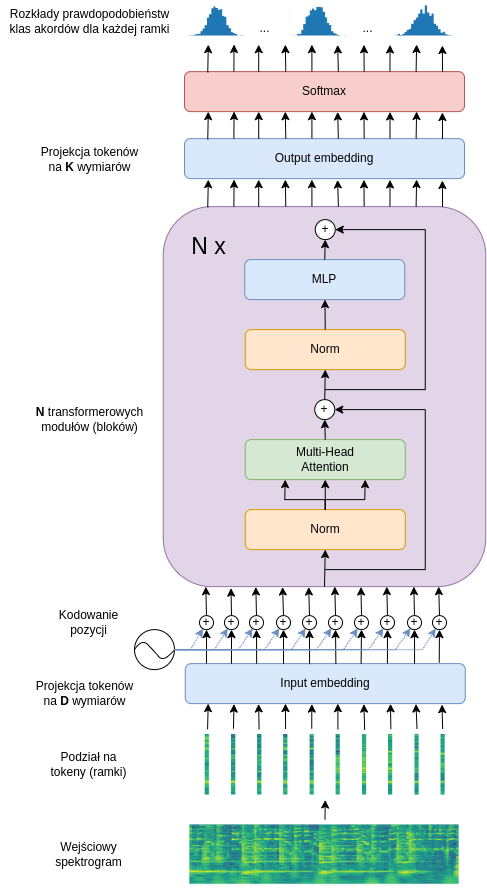
\includegraphics[width=0.8\textwidth]{./images/transformer.png}
    \caption{Schemat modelu transformera do rozpoznawania akordów muzycznych.}
    \label{fig:transformer}
\end{figure}

% ogólny opis architektury - wejście
Rysunek \ref{fig:transformer} prezentuje wykorzystany do treningów model sieci neuronowej --- transformer. Architektura tego modelu jest bardzo prosta. Na wejście sieci podawany jest składający się z $N$ ramek spektrogram $\defmatrix{S}{N}{F}$, który następnie dzielony jest (tylko ideowo, w~praktyce to wciąż pojedyncza macierz) na ramki (wektory $\vec s_i \in \mathbb{R}^F$). Ramki odgrywają rolę tokenów, czyli np. kolejnych słów w~przypadku przetwarzania języka naturalnego. Transformer przetwarza cały ciąg tokenów równolegle, co jest jego podstawową przewagą nad sieciami rekurencyjnymi, które przetwarzają ciąg tokenów w~sposób sekwencyjny. W~praktyce jednocześnie przez sieć może przejść kilka ciągów tokenów, czyli cały \emph{batch} sekwencji. Długość sekwencji tokenów jest zupełnie arbitralna, ten sam model może przetwarzać sekwencje różnej długości, zarówno w~treningu, jak i~później, podczas inferencji.

% ogólny opis architektury - input embedding i~positional encodding
W~pierwszej kolejności sekwencja ramek (macierz $\matrix{S}$) przechodzi przez pojedynczą warstwę liniową, która rzutuje tokeny wejściowe na wybraną dla danego modelu liczbę wymiarów $d_{\mathrm{model}}$:
\begin{equation}
    \matrix{T_{in}} = \matrix{S} \matrix{W_{in}}
\end{equation}
gdzie $\defmatrix{T_{in}}{N}{d_{\mathrm{model}}}$ to wyjściowa macierz tokenów a $\defmatrix{W_{in}}{F}{d_{\mathrm{model}}}$ to macierz parametrów tej warstwy. Liczba wymiarów $d_{\mathrm{model}}$, podobnie jak liczba tokenów $N$, nie zmienia się podczas przechodzenia przez kolejne warstwy, co różni transformer od sieci splotowych, gdzie rozmiar danych przechodzących przez sieć jest sukcesywnie zmniejszany. W~rzeczywistości istnieją architektury oparte o~oryginalny transformer, które podobnie jak sieć splotowa, zmniejszają rozmiar danych wejściowych, takie jak mniej dojrzałe \cite{liu_swin_2021}, czy też lepiej przemyślane \cite{dai_coatnet_2021}. Przed wejściem do stanowiących właściwą część transformera serii bloków, do tokenów dokładana jest informacja o~ich pozycji w~sekwencji --- jest to kodowanie pozycji (ang. \emph{positional encoding}). Szczegóły tej operacji zostały opisane poniżej.

% ogólny opis architektury - bloki, w~tym MLP i~normalizacja
Centralną część transformera stanowi ciąg identycznych bloków BLK. Liczba tych bloków ($B$), w~połączeniu z~wymiarowością tokenów ($d_{\mathrm{model}}$), stanowią główne hiperparametry modelu i~decydują o~jego rozmiarze. Każdy blok składa się z~dwóch głównych warstw: warstwy atencyjnej MSA (ang. \emph{Mulit-Head Self-Attention}) i~niewielkiego perceptronu wielowarstwowego MLP (ang.  \emph{Mulitlayer Perceptron}). Każdą z~tych warstw poprzedza normalizacja Norm typu \emph{Layer Normalization} \cite{ba_layer_2016}, a~kończy połączenie rezydualne \cite{he_deep_2015}, czyli dodanie do wartości na wyjściu nieznormalizowanej wartości z~wejścia. Operacje realizowane przez pojedynczy blok dla ciągu tokenów $\defmatrix{T}{N}{d_{\mathrm{model}}}$ można opisać równaniami:
\begin{eqnarray}
     \textrm{MSA}'(\matrix{T}) = \textrm{MSA}(\textrm{Norm}(\matrix{T})) + \matrix{T} \\
     \textrm{MLP}'(\matrix{T}) = \textrm{MLP}(\textrm{Norm}(\matrix{T})) + \matrix{T} \\
     \textrm{BLK}(\matrix{T}) = \textrm{MLP}'(\textrm{MSA}'(\matrix{T}))
\end{eqnarray}
Zastosowana normalizacja aplikowana jest niezależnie (choć równolegle) dla każdego tokena $t \in \mathbb{R}^{d_{\mathrm{model}}}$ z~sekwencji $\matrix{T}$. Polega ona na odjęciu wartości średniej tokena oraz podzieleniu przez jego odchylenie standardowe. Przedstawia to wzór:
\begin{equation}
    \textrm{Norm}(t) = \frac{t - \textrm{E}[t]}{\sqrt \textrm{Var}[t]} \cdot \gamma + \beta
\end{equation}
gdzie $\gamma$ i $\beta$ to trenowane parametry warstwy, przesuwające i~skalujące odpowiednio wynik normalizacji. Jeżeli chodzi o~perceptron wielowarstwowy, to ma on zawsze dwie warstwy ukryte, z~wymiarem ukrytym czterokrotnie większym niż $d_{\mathrm{model}}$ oraz funkcją aktywacji GELU.
\begin{equation}
    \textrm{MLP}(\matrix{T}) = \textrm{GELU}(\matrix{T}\matrix{W_1} + b_1)\matrix{W_2} + b_2
\end{equation}
gdzie wejściem jest sekwencja tokenów $\defmatrix{T}{N}{d_{\mathrm{model}}}$, macierze $\defmatrix{W_1}{d_{\mathrm{model}}}{4d_{\mathrm{model}}}$, $\defmatrix{W_2}{4d_{\mathrm{model}}}{d_{\mathrm{model}}}$ oraz wektory (dodawane do każdego wiersza odpowiedniej macierzy) $b_1 \in \mathbb{R}^{4d_{\mathrm{model}}}$ i $b_2 \in \mathbb{R}^{d_{\mathrm{model}}}$ to parametry dwóch warstw ukrytych perceptronu wielowarstwowego.

% ogólny opis architetury - dropout
W~rzeczywistości pojedynczy blok zawiera jeszcze jeden opcjonalny element, jakim są warstwy \emph{dropout}, umieszczone w~trzech miejscach: po funkcji aktywacji w~module MLP oraz po każdym z~dwóch połączeń rezydualnych, czyli w~połowie bloku i~na jego wyjściu. Dodatkowo \emph{dropout} może być stosowany również przed wejściem do sieci, czyli bezpośrednio na spektrogramie. Warstwy tego typu zerują z~wybranym prawdopodobieństwem niektóre z~przechodzących przez nie wartości w~celu regularyzacji sieci i~uniknięcia przetrenowania. Technika ta jest opcjonalna i~nie była stosowana we wszystkich eksperymentach.

% ogólny opis architektury - wyjście (klasyfikacja)
Po serii bloków następuje ostatnia część modelu, odpowiedzialna za klasyfikację. Najpierw, utrzymywana przez wszystkie bloki, wymiarowość tokenów jest zmieniana przez warstwę liniową, w~zależności od liczby klas $K$.
\begin{equation}
    \matrix{T_{out}} = \matrix{T} \matrix{W_{out}}
\end{equation}
gdzie $\defmatrix{T_{out}}{N}{K}$ to macierz wyjściowa, $\defmatrix{T}{N}{d_{\mathrm{model}}}$ to macierz sekwencji tokenów a $\defmatrix{W_{out}}{d_{\mathrm{model}}}{K}$ to macierz parametrów tej warstwy liniowej. Następnie dla każdego tokena $t \in \mathbb{R}^K$ zwracany jest rozkład prawdopodobieństwa przynależności do poszczególnych klas akordów, za pomocą funkcji \emph{softmax}:
\begin{equation}
    \textrm{softmax}(t_i) = \frac{\exp{t_i}}{\sum_{j=1}^{K}\exp{t_j}}
\end{equation}
gdzie $t_i$ to $i$-ty element wektora (tokena) $t$. Podsumowując, na wejściu sieci jest spektrogram, składający się z $N$ ramek i $F$ cech, a~na wyjściu jest $N$ rozkładów prawdopodobieństwa między $K$ klas, dla każdej z~ramek spektrogramu. Wszystkie ramki spektrogramu są więc klasyfikowane jednocześnie, ale z~uwzględnieniem kontekstu, jaki tworzą razem.

\subsection{Kodowanie pozycji tokenów}

% positional encoding
Jak widać na rysunku \ref{fig:transformer}, pomiędzy projekcją tokenów wejściowych a~wejściem do serii bloków, jest jeszcze etap kodowania pozycji każdego z~tokenów. Etap ten jest niezbędny, aby zawrzeć w każdym z~tokenów informację o~tym, jaka jest jego pozycja w~sekwencji. W~przypadku sieci rekurencyjnych informacja ta jest zawarta niejawnie, poprzez przetwarzanie tokenów jeden po drugim, w~odpowiedniej kolejności. W~przypadku transformerów, gdzie tokeny są przetwarzane równolegle, informacja ta musi być dodana jawnie.  Istnieje wiele sposobów, według których można zakodować pozycję tokenów, głównie dzielących się na wykorzystanie wartości wyuczonych (parametry modelu) i~stałych (odpowiednia funkcja).  W~niniejszej pracy wykorzystane zostało podejście oryginalnych twórców transformera, oparte o~wartości funkcji sinus i~kosinus. Polega ono na tym, że dla każdego tokena (dla każdej pozycji) generuje się wektor, który ma tę samą liczbę wymiarów co token, dzięki czemu może być do niego dodany. Wartości tych wektorów zdefiniowane są wzorami:
\begin{equation}
    PE_{(\textrm{pos},2i)} = \sin(\textrm{pos}/10000^{2i/d_{\textrm{\tiny model}}})
\end{equation}
\begin{equation}
PE_{(\textrm{pos},2i + 1)} = \cos(\textrm{pos}/10000^{2i/d_{\textrm{\tiny model}}})
\end{equation}
Równania te oznaczają, że każdy wymiar wektora kodującego pozycję odpowiada sinusoidzie o~innej częstotliwości. Parzyste pozycje w~wektorze to wartości odpowiednich funkcji sinus dla danej pozycji, a~nieparzyste to wartości funkcji kosinus dla danej pozycji. Stosowany jest również wariant, gdzie pierwsza połowa wektora to wartości funkcji sinus a~druga to wartości funkcji kosinus. Autorzy uzasadniają, że użycie tych funkcji pozwala modelowi łatwo wykorzystywać informację o~pozycji, ponieważ między wektorami prezentującymi różne pozycje występują zależności liniowe. Na rysunku \ref{fig:positional_encoding} przedstawiono graficzną reprezentację wektorów kodujących pozycję, dla sekwencji składającej się ze 100 tokenów (wiersze), gdzie liczba wymiarów każdego z~nich to 256 (kolumny).
\begin{figure}
    \centering
    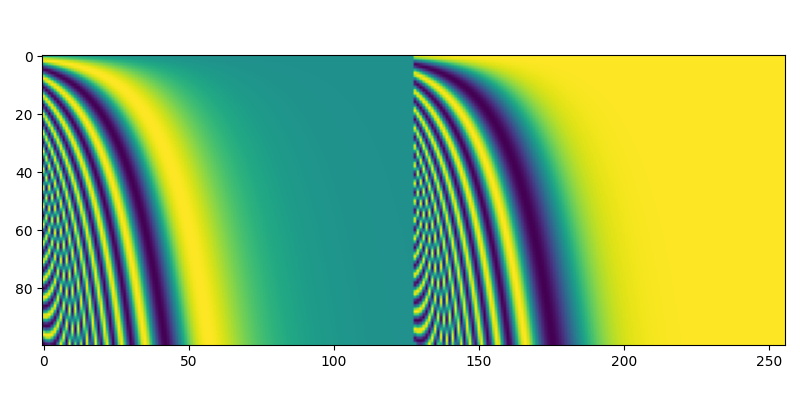
\includegraphics[width=1.0\textwidth]{./images/positional_encoding.png}
    \caption{Przykład wektorów kodujących pozycję dla sekwencji 100 tokenów o~wymiarowości 256.}
    \label{fig:positional_encoding}
\end{figure}

\subsection{Multi-Head Self-Attention}

% mutli-head self-attention - wstęp
Najważniejszą część transformera stanowi warstwa atencyjna MSA. Jako jedyna w~całym modelu odpowiada ona za ,,wymianę'' informacji między tokenami --- uwzględnienie kontekstu pozostałych tokenów w~sekwencji, podczas tworzenia nowej reprezentacji danego tokena.

% mutli-head self-attention - ogólnie o~mechaniźmie attention
Sama idea mechanizmu \emph{Attention} polega na tym, że mając dla danego tokena wejściowego zapytanie (ang. \emph{query}) i~mając zbiór par klucz-wartość (ang. \emph{key-value}) związanych z~innym (lub tym samym) ciągiem tokenów, wylicza się nową reprezentację tokena jako ważoną sumę tych wartości, gdzie wagi są wyliczane na podstawie dopasowania zapytania do kluczy. Wagi te informują więc o~tym, jak dużo uwagi powinno poświęcić się danej wartości, tworząc nową reprezentację danego tokena. W~przypadku zadania tłumaczenia maszynowego mechanizm ten pozwala skupić się na odpowiednich częściach sekwencji wejściowej, podczas tworzenia sekwencji wyjściowej. Jeżeli zarówno zapytania, jak i~pary klucz-wartość pochodzą z~tej samej sekwencji tokenów, mamy do czynienia z \emph{Self-Attention}. Warstwa tego typu wyznacza więc dla każdego tokena w~sekwencji zapytanie, klucz i~wartość, a~następnie tworzy jego nową reprezentację, jako ważoną sumę wartości pozostałych tokenów. Informacje zakodowane w~poszczególnych tokenach mieszają się zatem między sobą. W~praktyce warstwa atencyjna w~transformerze realizuje równolegle kilka niezależnych operacji \emph{Self-Attention}, których wyniki na końcu są łączone w~całość, stąd też nazwa \emph{Multi-Head Self-Attention}. Pozwala to uzyskać lepsze rezultaty niż pojedyncza operacja, nawet jeżeli wykorzysta się niżej wymiarowe reprezentacje.

% mutli-head self-attention - dokładnie jak działa, wzorki
Na wejściu warstwy atencyjnej w~transformerze znajduje się macierz $\defmatrix{T}{N}{d_{\mathrm{model}}}$, czyli sekwencja $N$ tokenów. Dla każdego z~nich, za pomocą zwykłych warstw liniowych, wylicza się $H$-krotnie trzy wektory: zapytanie $q_i \in \mathbb{R}^{d_k}$, klucz $k_i \in \mathbb{R}^{d_k}$ oraz wartość $v_i \in \mathbb{R}^{d_v}$, gdzie $i \in [1, H]$. Dla całej sekwencji tokenów wektory te tworzą macierze $\defmatrix{Q_i}{N}{d_k}$, $\defmatrix{K_i}{N}{d_k}$ oraz $\defmatrix{V_i}{N}{d_v}$. Przedstawiają to równania:
\begin{eqnarray}
    \matrix{Q_i} = \matrix{T} \matrix{W_i^Q} \\
    \matrix{K_i} = \matrix{T} \matrix{W_i^K} \\
    \matrix{V_i} = \matrix{T} \matrix{W_i^V}
\end{eqnarray}
gdzie macierze $\defmatrix{W_i^Q}{d_{\mathrm{model}}}{d_k}$, $\defmatrix{W_i^K}{d_{\mathrm{model}}}{d_k}$ oraz $\defmatrix{W_i^V}{d_{\mathrm{model}}}{d_v}$ to macierze parametrów warstw liniowych tworzących $i$-tą trójkę: zapytanie, klucz i~wartość.

Dla pojedynczej trójki macierzy $\matrix{Q}$, $\matrix{K}$ i $\matrix{V}$ operacja \emph{Self-Attention} wygląda następująco:
\begin{equation} \label{eq:sa}
    \textrm{SA}(\matrix{Q}, \matrix{K}, \matrix{V}) = \textrm{softmax}(\frac{\matrix{Q}\matrix{K^T}}{\sqrt{d_k}})\matrix{V}
\end{equation}
gdzie $\matrix{K^T}$ oznacza transpozycję macierzy $\matrix{K}$. Człon ,,$\textrm{softmax}(\frac{\matrix{Q}\matrix{K^T}}{\sqrt{d_k}})$'' oznacza wyliczenie macierzy atencji między wszystkimi parami klucz-zapytanie, poprzez wykonanie iloczynów skalarnych dla każdej z~tych par, przeskalowanie uzyskanych wartości i~wykorzystanie normalizującej funkcji \emph{softmax}. Dlatego też funkcja SA nazywa się właściwie \emph{Scaled Dot-Product Attention}.  Wartości w~uzyskanej macierzy atencji odgrywają rolę wag, które następnie są użyte do stworzenia nowej reprezentacji wszystkich tokenów, za pomocą średniej ważonej wektorów z~macierzy $\matrix{V}$.  Wynik operacji SA jest więc macierzą, o~wymiarach $N \times d_v$.

Cała operacja \emph{Multi-Head Self-Attention} polega na $H$-krotnym wykonaniu operacji \emph{Self-Attention}, których wektory wynikowe są łączone i~ostatecznie rzutowane z~powrotem na $d_{\mathrm{model}}$ wymiarów. Przedstawiają to poniższe wzory:
\begin{equation}
    \textrm{MSA}(\matrix{T}) = \textrm{Concat}(\textrm{SA}(\matrix{Q_1}, \matrix{K_1}, \matrix{V_1}), ..., \textrm{SA}(\matrix{Q_H},
    \matrix{K_H}, \matrix{V_H}))\matrix{W^O}
\end{equation}
gdzie macierz $\defmatrix{W^O}{Hd_v}{d_{\mathrm{model}}}$ to parametry ostatniej w~ramach bloku atencyjnego warstwy liniowej, która rzutuje sklejone wektory z~pojedynczych operacji SA na początkowe $d_{\mathrm{model}}$ wymiarów. Dzięki temu wymiarowość tokenów na wyjściu z~warstwy atencyjnej pozostaje taka sama jak na wejściu. W~niniejszej pracy zastosowane zostało powszechne podejście, aby liczbę wymiarów wektorów zapytań, kluczy i~wartości ustalić z~góry i~uzależnić od liczby wymiarów tokenów i~liczby równoległych operacji SA. Zależność ta jest następująca:
\begin{equation}
    d_k = d_v = \frac{d_{\mathrm{model}}}{H}
\end{equation}
Wszystkimi parametrami podlegającymi adaptacji w~ramach warstwy MSA, są parametry czterech opisanych powyżej, pomocniczych warstw liniowych --- $\matrix{W_i^Q}$, $\matrix{W_i^K}$, $\matrix{W_i^V}$ i $\matrix{W^O}$. Poza wspomnianymi wcześniej hiperparametrami $B$ i $d_{\mathrm{model}}$ istotna dla funkcjonowania modelu jest również liczba $H$ równoległych operacji SA, nazywana również ,,liczbą głów''. Wszystkie hiperparametry transformera zostały zebrane w~Tab. \ref{tab:transformer_params}.

\begin{table}
    \centering
    \caption{Hiperparametry transformera.}
    \label{tab:transformer_params}
    \begin{tabular}{|c|l|} \hline
        Symbol & Znaczenie \\ \hline
        $F$ & Wymiarowość na wejściu \\
        $d_{\mathrm{model}}$ & Wymiarowość tokenów wewnątrz sieci \\
        $B$ & Liczba bloków transformera \\
        $H$ & Liczba ,,głów'' w~bloku MSA \\
        $K$ & Liczba klas na wyjściu \\
        $p_d$ & Prawdopodobieństwo warstw \emph{dropout} \\ \hline
    \end{tabular}
\end{table}

\subsection{Dwukierunkowy transformer do rozpoznawania akordów --- BTC}

W~pracy referencyjnej \cite{park_bi-directional_2019} autorzy postanowili wprowadzić drobne modyfikacje w~stosunku do oryginalnego bloku transformera, tworząc swój autorski model nazwany \emph{bi-directional transformer for chord recognition} (BTC). Pierwszą z~nich jest zamiana dwóch warstw liniowych w~module MLP, na dwie jednowymiarowe warstwy splotowe z~polem recepcyjnym szerokości 3~tokenów. Liczba kanałów w~tych warstwach splotowych jest stała i~równa wymiarowości tokenów. Według autorów ma to ułatwić sieci tworzenie bardziej ,,wygładzonych'' predykcji i~lepsze wykorzystanie kontekstu otaczającego każdą ramkę. Druga różnica polega na tym, że pojedynczy blok transformerowy został rozbity na dwa, które dostają te same wartości na wejściu, a~ich wartości wyjściowe są łączone za pomocą dodatkowej warstwy liniowej. Bloki te różnią się operacją MSA.  Została w~nich zastosowana technika maskowania, polegająca na modyfikacji macierzy atencji (wzór \ref{eq:sa}) w~ten sposób, że dla danego tokena, wagi wszystkich wcześniejszych tokenów (dla pierwszego bloku) lub wszystkich późniejszych tokenów (dla drugiego bloku) są zerowane. Oznacza to, że tworząc nową reprezentację danego tokena, wykorzystuje się jedynie tokeny poprzedzające, lub następujące po nim. W~modelu BTC każdy z~dwóch bloków tworzących moduł MSA ma inny kierunek maskowania. Technika ta ma zmusić model do pełnego wykorzystywania zarówno wcześniejszego, jak i~późniejszego kontekstu przy klasyfikacji danej ramki. Poza uproszczonym, pozbawionym powyższych usprawnień modelem transformera, w~niniejszej pracy zaimplementowany został również model oparty o~bloki BTC. Wykorzystany został on w~pojedynczym eksperymencie, aby zreprodukować wyniki z~pracy referencyjnej i~zbadać znaczenie wspomnianych modyfkacji.



\section{Treningi nadzorowane}

% wstęp
Pierwszy z~dwóch rodzajów wykonywanych treningów sieci to klasyczny trening nadzorowany.  Wykorzystywane są w~nim dane z~oznaczeniami, aby nauczyć model rozwiązywania konkretnego problemu --- klasyfikacji akordów muzycznych. 

% TODO: parę słów o~koncepcji treningów nadzorowanych

\subsection{Procedura treningu}

% walidacja krzyżowa, zbiory i~epoki
W~ramach niniejszej pracy, do oceny jakości modeli wykorzystana została pięciokrotna walidacja krzyżowa. Oznacza to, że pojedynczy eksperyment, związany z~pojedynczym zestawem hiperparametrów modelu, zbioru danych i~treningu, składa się z~pięciu treningów. W~każdym z~nich jedna z~pięciu części zbioru danych wykorzystana jest do walidacji, a~pozostałe cztery do nauki. Możliwe jest, aby ograniczyć cały zbiór danych do wybranych zbiorów oznaczeń (np. Isophonics, czy Billboard), co zupełnie nie zmienia zasady działania walidacji krzyżowej, ponieważ w~ramach każdego zbioru oznaczeń zachowany jest podział na pięć równych części. Treningi dzieli się na epoki, które z~definicji oznaczają pojedyncze przejście przez wszystkie dostępne dane treningowe (w tym przypadku cztery z~pięciu części zbioru). Jak opisano w~rozdziale \ref{sec:preprocessing}, w~przypadku przeprowadzonych eksperymentów, pojedyncza epoka oznacza kilkukrotne przejście przez wszystkie utwory treningowe, ale dla każdego utworu przetwarzany jest jedynie jego losowy fragment (lub fragmenty).

% kroki
Na epokę składają się kroki, gdzie każdy krok oznacza jedną zmianę parametrów modelu. W~ramach każdego kroku model przetwarza równolegle cały \emph{batch} 10-sekundowych fragmentów utworów.  Ponieważ, ze względów optymalizacyjnych, na jeden przykład ze zbioru danych składa się kilka fragmentów tego samego utworu, to na realny rozmiar \emph{batcha} wpływają dwa hiperparametry: liczba analizowanych równolegle przykładów (czyli utworów) oraz liczba zwracanych jednocześnie fragmentów pojedynczego utworu. Dla każdej ramki, z~każdego fragmentu wejściowego, model zwraca predykcję akordów, w~postaci rozkładów prawdopodobieństw. Rozkłady te są następnie porównywane z~rzeczywistymi klasami akordów za pomocą funkcji kosztu, jaką jest entropia krzyżowa (ang. \emph{cross-entropy}). Dla pojedynczej ramki, czyli dla pojedynczego wyjściowego rozkładu prawdopodobieństw $t \in \mathbb{R}^K$ i~indeksu $k$, oznaczającego numer rzeczywistej klasy tej ramki, entropia krzyżowa ma postać:
\begin{equation}
    \textrm{CE}(t, k) = - \log t_k
\end{equation}
Wartość tę uśrednia się później między wszystkimi tokenami (ramkami) i~między sekwencjami (fragmentami), aby uzyskać pojedynczą liczbę rzeczywistą, reprezentującą błąd popełniany przez sieć.  Następnie, zgodnie z~algorytmem \emph{backpropagation}, obliczane są pochodne cząstkowe (gradient) tej funkcji kosztu po wszystkich parametrach modelu. Do optymalizacji parametrów modelu na podstawie obliczonych pochodnych wykorzystany jest algorytm optymalizacyjny \emph{AdamW}. Współczynnik nauki (ang. \emph{learning rate}), przez pierwszych pięć epok ma jedynie dziesiątą część swojej docelowej wartości, aby zapewnić małe zmiany parametrów modelu na początku treningu. Transformery są bowiem podatne na to, że z~powodu zbyt dużych kroków w~początkowej fazie treningu, przestaną zbiegać do konkretnego rozwiązania. Co więcej, na potrzeby późniejszej analizy, w~każdym kroku zapisywane są wartości funkcji kosztu i~metryki \emph{accuracy} dla obecnego \emph{batcha} przykładów.

\subsection{Walidacja i~wczesne zatrzymanie treningu}

% walidacja i~wczesne zatrzymanie
Pod koniec każdej epoki, po przejściu przez całą część treningową (cztery z~pięciu części), następuje bieżąca ocena modelu na części walidacyjnej (ostatnia z~pięciu części). Celem tego etapu jest zobaczyć, jak model radzi sobie z~przykładami, na których nie był uczony. Można w~ten sposób rozpoznać moment, kiedy sieć zaczyna się przetrenowywać i~zatrzymać trening (ang. \emph{early stopping}). Aby zapewnić stabilność wyników tej oceny, nie stosuje się w~niej, tego samego co podczas nauki, mechanizmu losowania fragmentów utworów. Nie stosuje się również augmentacji. Zamiast tego, dla każdego utworu wykonuje się po kolei predykcję klas dla wszystkich ramek. Szczegóły procedury predykcji klas akordów dla całego utworu zostały opisane poniżej. Mając dla danego utworu predykcję wszystkich akordów, oblicza się na tej podstawie wartość metryki \emph{accuracy}. Po przejściu przez całą część walidacyjną, \emph{accuracy} wyliczane jest jeszcze raz, ale dla wszystkich utworów ze zbioru walidacyjnego jednocześnie (dla jednego długiego ciągu predykcji). Podczas przechodzenia przez kolejne epoki, zapamiętywana jest najlepsza wartości \emph{accuracy}, wraz z~numerem danej epoki i~aktualnym stanem modelu. Jeżeli wartość \emph{accuracy} nie wzrasta przez zadaną liczbę epok, trening zostaje wstrzymany.

\subsection{Ewaluacja modelu} \label{subsection:model_evaluation}

% ewaluacja
Po wstrzymaniu treningu z~powodu przetrenowania modelu lub po przejściu przez zadaną liczbę epok model zostaje przywrócony do stanu, dającego najlepsze wyniki na części walidacyjnej. Następnie na tejże części wykonywana jest bardziej dogłębna ocena wytrenowanej sieci. Polega ona, podobnie jak podczas treningu, na wytworzeniu predykcji, na podstawie których, dla każdego utworu wyliczane są dodatkowo: 
\begin{itemize}
    \item ciąg wystąpień akordów (\code{ChordOccurence}), o~określonym czasie rozpoczęcia i
        zakończenia w~sekundach (ciąg takich samych predykcji jest łączony w~jedno wystąpienie
        akordu)
    \item wartość miary CSR (ang. \emph{Chord Symbol Recall}) na podstawie
        ciągu wystąpień akordów, która ma postać
        \begin{displaymath}
            \textrm{CSR} = \frac
                        {\textrm{całkowity czas trwania poprawnie zaklasyfikowanych fragmentów}}
                        {\textrm{całkowity czas trwania utworów}}
        \end{displaymath}
    \item wartości miar klasyfikacyjnych, liczonych tak, że pojedyncza ramka jest traktowana, jak
        pojedyncza predykcja:
        \begin{itemize}
            \item dokładność (ang. \emph{accuracy}; $1$ wartość)
            \item czułość (ang. \emph{recall}) per klasa ($25$ wartości)
            \item precyzja (ang. \emph{precision}) per klasa ($25$ wartości)
            \item macierz pomyłek (ang. \emph{confusion matrix})
        \end{itemize}
\end{itemize}
Ciąg wystąpień akordów zapisywany jest w~pliku \filetype{lab}, a~wartości metryk CSR, dokładności, czułości, precyzji i~macierz pomyłek w~pliku \filetype{json}. Dodatkowo macierz pomyłek zapisywana jest jako obrazek w~pliku \filetype{png}. Następnie wartości wszystkich tych miar są agregowane dla wszystkich utworów ze zbioru walidacyjnego i~również zapisywane w~plikach \filetype{json} i \filetype{png}. Miary klasyfikacjne agregowane są poprzez wyliczenie ich jeszcze raz na jednym, długim, połączonym ciągu predykcji, pochodzących ze wszystkich utworów. Jeżeli chodzi o~wartości miary CSR, to aby zagregować ją dla wszystkich utworów liczy się średnią ważoną, gdzie wagą jest długość trwania utworu --- miara ta nazywa się wtedy WCSR (ang. \emph{Weighted Chord Symboll Recall}). Co do zapisywanej na obrazku ,,globalnej'' macierzy pomyłek, to jest ona normalizowana wierszami, czyli wartości na głównej przekątnej są równoważne czułości modelu dla danej klasy. Implementacja całej procedury ewaluacji modelu znajduje się w~pliku \url{src/training/evaluate.py}.

% problem podwójnego wykorzystania zbioru walidacyjnego + uzasadnienie wykorzystania walidacji krzyżowej
Jak można zauważyć, część walidacyjna jest w~pojedynczym treningu wykorzystywana na dwa sprzeczne sposoby. Po pierwsze służy do oceny jakości modelu na koniec procesu nauki. Jest to więc typowe zastosowanie, zgodne z~zasadami walidacji krzyżowej. Z~drugiej jednak strony, ten sam zbiór jest wykorzystywany do wykrycia przetrenowania i~wczesnego zatrzymania treningu. Prowadzi to do swego rodzaju ,,przetrenowania'' pod część walidacyjną, ponieważ wybierany jest ten stan modelu, który wiadomo, że daje najlepsze wyniki dla danych przykładów. W~takich sytuacjach, kiedy nie stosuje się walidacji krzyżowej, standardowo dzieli się zbiór na trzy części: treningową do nauki, testową do ostatecznej oceny i~walidacyjną do oceny podczas treningu i~uniknięcia przetrenowania. Technikę tę --- dzielenie zbioru na trzy części --- można zastosować również dla walidacji krzyżowej, jeżeli jest to konieczne. W~przypadku tej pracy zostało to jednak uznana za zbędne, z~tego powodu, że właściwym celem oceny modeli jest porównanie ich między sobą, a~nie poznanie jak najlepszego przybliżenia ich rzeczywistej dokładności (rola zupełnie odrębnego zbioru testowego). Fakt, że każdy z~nich daje nieznacznie zawyżone wyniki na części walidacyjnej, nie utrudnia porównania ich między sobą. Najważniejsze jest to, że walidacja krzyżowa pozwala uniknąć problemu obciążenia pojedynczego, niewielkiego zbioru testowego. Obciążenie takie, charakterystyczne dla zbyt małego, niereprezentatywnego zbioru, uniemożliwia rzetelne porównanie modeli między sobą. Łatwo może wtedy bowiem dojść do sytuacji, kiedy model wydaje się lepszy od innych, bo przypadkowo daje lepsze wyniki na małym zbiorze testowym, choć dla przykładów spoza tego zbioru radzi sobie znacznie gorzej.

\subsection{Implementacja i~wykorzystana infrastruktura}

% implementacja i~sprzęt
Pętla treningowa została zaimplementowana w~pliku \url{src/training/training.py}. Została ona przygotowana w~taki sposób, aby można było trenować modele w~sposób rozproszony, zgodnie z~techniką \emph{Distributed Data Parallel}. Do rejestrowania treningów, ich hiperparametrów i~wartości metryk wykorzystano system \emph{MLflow}\footnote{\url{https://mlflow.org/}}. Treningi odbywały się na jednej lub kilku kartach graficznych NVIDIA GeForce RTX 3090.

\subsection{Podsumowanie hiperparametrów treningu}

% podsumowanie hiperparametrów treningu
Wszystkie ustawienia pojedynczej serii pięciu treningów (eksperymentu), włączając w~to ustawienia zbioru danych, hiperparametry modelu i~hiperparametry samej pętli treningowej, zostały przedstawione w~Tab. \ref{tab:sup_training_params}. Wartości hiperparametrów z~tej tabeli są wymieniane dla każdego udokumentowanego eksperymentu. W~rzeczywistości przygotowana implementacja umożliwia również zmianę hiperparametrów, które zostały wybrane jako niezmienne dla niniejszej pracy i~opisane w~rozdziale \ref{sec:preprocessing}, takich jak długość przetwarzanego przez model fragmentu (100 ramek). Te hiperparametry nie zostały wymienione w~tabeli, ponieważ nie różnią się między eksperymentami. Pominięte również zostały hiperparametry o~charakterze ściśle technicznym, takie jak wykorzystanie pamięci podręcznej w~RAM-ie, czy wykorzystanie treningu rozproszonego.

% wszystkie hiperparametry wynikające z~argparse (F-fixed, T-technical, X-changed between experiments)
% DATASET
% F   sample_rate=22050
% F   frame_size=2048
% F   hop_size=2048
% F   frames_per_item=100
% X   item_multiplier
% X   song_multiplier
% F   audio_preprocessing (cqt, raw)=CQT
% F   standardize_audio=YES
% X   pitch_shift_augment
% F   labels_vocabulary=MAJ_MIN
% X   subsets
% X   dataset_fraction (TODO: opisać w~rozdziale o~datasecie)
% T   use_ram_cache
% MODEL
% X   model_dim
% X   n_heads
% X   n_blocks
% X   block_type
% X   dropout_p
% T   extra_features_dim=NO
% T   pretrained_encoder_path
% T   pretrained_encoder_run_name
% TRAINING
% T   experiment_name
% T   run_name
% X   n_epochs
% X   batch_size
% X   lr
% X   early_stopping
% T   ddp
% T   num_workers

\begin{table}
    \centering
    \caption{Hiperparametry pojedynczego treningu nadzorowanego.}
    \label{tab:sup_training_params}
    \begin{tabular}{|l|p{0.6\linewidth}|} \hline
        \multicolumn{2}{|c|}{ZBIÓR DANYCH} \\ \hline
        \code{item\_mutliplier} & Liczba przykładów zwracanych dla jednego utworu \\
        \code{song\_multiplier} & Liczba przejść przez wszystkie utwory w~jednej epoce \\
        \code{augment} & Czy zastosowano augmentacje \\
        \code{subsets} & Jakie podzbiory zostały wykorzystane do treningu \\
        \code{fraction} & Jaka część zbioru treningowego została wykorzystana do treningu \\ \hline
        \multicolumn{2}{|c|}{MODEL} \\ \hline
        \code{model\_dim} & Liczba wymiarów pojedynczego tokena przechodzącego przez model \\
        \code{n\_heads} & Liczba równoległych operacji MSA \\
        \code{n\_blocks} & Liczba bloków w~modelu \\
        \code{block\_type} & Typ bloku: BTC lub zwykły transformer \\
        \code{dropout\_p} & Prawdopodobieństwo zerowania w~warstwach \emph{dropout} \\ \hline
        \multicolumn{2}{|c|}{TRENING} \\ \hline
        \code{n\_epochs} & Liczba epok w~treningu \\
        \code{batch\_size} & Liczba utworów przetwarzanych w~jednym kroku \\
        \code{lr} & Współczynnik uczenia \\
        \code{early\_stopping} & Maksymalna liczba epok bez wzrostu dokładności na części walidacyjnej \\ \hline
    \end{tabular}
\end{table}

\subsection{Zasady predykcji akordów dla całego utworu}

Najprostszym sposobem, aby uzyskać predykcję dla całego utworu, który zazwyczaj składa się z~kilku tysięcy ramek, jest podanie wszystkich ramek jednocześnie na wejście sieci neuronowej. O~ile transformer może teoretycznie przyjąć na wejściu sekwencję dowolnej długości (ograniczeniem jest oczywiście pamięć), to w~przypadku sekwencji dłuższych niż w~treningu, wymaga to od modelu pewnej generalizacji. Jest to więc podejście ryzykowne i~mało praktyczne, ze względu na ograniczenie pamięci, które w~praktyce może spowodować, że i~tak będzie trzeba dzielić utwór na kilka części.

Najbezpieczniej podawać więc na wejście modelu fragmenty takiej długości jak w~treningu, czyli po $100$ ramek na raz. Pozostaje zdecydować, czy fragmenty mają się na siebie nakładać i~jeśli tak, to w~jaki sposób agregować kilka możliwych predykcji dla jednej ramki. W~niniejszej pracy zdecydowano się na takie podejście, zgodnie z~którym z~każdej $100$-elementowej sekwencji, jedynie środkowe $50$ branych jest do ostatecznego wyniku. Pozostałe $25$ ramek z~początku i $25$ ramek z~końca traktowane są jako kontekst. Wynika to z~niezweryfikowanej hipotezy, że predykcje dla ramek z~szerszym kontekstem przed nimi i~po nich, są precyzyjniejsze, niż dla ramek na brzegu fragmentu, dla których nie wiadomo dobrze, co działo się przed nimi lub po nich. Oznacza to w~praktyce, że kolejne fragmenty nakładają się na siebie w~połowie. 

Cała procedura wytwarzania predykcji dla pojedynczego nagrania polega więc na:
\begin{itemize}
    \item podzieleniu nagrania na rozłączne fragmenty po $50$ ramek;
    \item dodaniu do każdego fragmentu po $25$ ramek z~fragmentów wcześniejszego i~późniejszego, w
        przypadku pierwszego i~ostatniego fragmentu, uzupełnić powtórzoną wielokrotnie odpowiednio
        pierwszą i~ostatnią ramką;
    \item wykonaniu predykcji dla wszystkich utworzonych w~ten sposób fragmentów, po $100$ ramek
        każdy;
    \item wyciągnięciu $50$ środkowych akordów z~każdej sekwencji wyjściowej i~złączeniu ich w~jedną
        sekwencję, o~długości równej liczbie ramek utworu.
\end{itemize}
Mechanizm ten, w~ogólnej postaci, zaimplementowany został w~funkcji \code{partial\_predict} w~pliku \url{src/training/evaluate.py}. W~rzeczywistości, wszystkie nakładające się na siebie fragmenty, są przetwarzane przez model równolegle, jako jeden \emph{batch} przykładów.

Proporcja między długością pojedynczego fragmentu ($100$ ramek) a~długością kontekstu (po $25$ ramek przed i~po), została ustalona na podstawie intuicji. Nie przeprowadzono żadnej dokładnej analizy ani eksperymentów, aby ustalić, jaki ma ona wpływ na jakość predykcji. Możliwe jest zarówno to, że bez nakładania na siebie fragmentów, predykcje nie byłyby w~ogóle (lub znacząco) gorsze, jak i~to, że zwiększenie długości kontekstu, poprawiłoby istotnie predykcje sieci.



\section{Samonadzorowane treningi wstępne}

% wstęp - co to self-supervised - ogólna koncepcja (TODO: czy to tutaj czy nie?)
Nienadzorowany, a~dokładnie samonadzorowany (ang. \emph{self-supervised}) trening wstępny, stanowi kluczową część niniejszej pracy. Algorytmy tego typu polegają na wykonywaniu przez sieć specjalnego, dodatkowego zadania pomocniczego (ang. \emph{pretext task}), w~wyniku którego model uczy się ekstrahować wysokopoziomowe, abstrakcyjne, bogate semantycznie cechy. Treningi takie zbudowane są dokładnie tak samo, jak treningi nadzorowane, ale samo zadanie (wraz z~oznaczeniami) jest wytworzone sztucznie i~nie wymaga oznaczeń przygotowanych przez człowieka. Przykładem może być układanie przez sieć neuronową puzzli \cite{noroozi_unsupervised_2017}, dorysowywanie brakującego fragmentu rysunku \cite{pathak_context_2016}, czy też uzupełnianie słów w~zdaniach \cite{devlin_bert_2019}. Algorytmów tych jest bardzo wiele i~można podzielić je na wiele różnych rodzajów, które wykorzystywane są dla różnych typów danych (czasami kilku jednocześnie \cite{jia_scaling_2021}). Ze względu na ogromną dostępność danych nieoznaczonych (Internet), metody tego typu zyskują bardzo na popularności w~ostatnich latach. W~dziedzinach przetwarzania języka naturalnego i~rozpoznawania mowy są już właściwie standardem. Wytrenowany za pomocą takich metod model, może być później dotrenowany (ang. \emph{fine-tuning}) w~sposób nadzorowany, na zbiorze danych związanym z~konkretnym zadaniem. Jeżeli trening wstępny się udał, może przynieść on różnego rodzaju zysk dla zadania docelowego, w~porównaniu do treningu od zera. Przykładami są:
\begin{itemize}
    \item krótszy wymagany czas treningu nadzorowanego;
    \item mniejszy wymagany zbiór danych oznaczonych;
    \item mniejsza podatność na przetrenowanie;
    \item lepsza generalizacja i~w ogóle lepsza ostateczna jakość modelu.
\end{itemize}

% wstęp - jaki zastosowano algorytm - ogólna idea, że na podstawie MAE, BERT, wav2vec
Zastosowany w~ramach niniejszej pracy algorytm uczenia samonadzorowanego, stanowi autorską adaptację algorytmu MAE (ang. \emph{Masked Auto-Encoders}) \cite{he_masked_2021}, pochodzącego z~obszaru przetwarzania obrazów. Algorytm MAE ma naturę bardzo ogólną i~sam jest właściwie adaptacją oryginalnego algorytmu BERT \cite{devlin_bert_2019}, stosowanego w~dziedzinie przetwarzania języka naturalnego. Bardzo podobnym rozwiązaniem z~dziedziny rozpoznawania mowy jest również \cite{baevski_wav2vec_2020}. Wszystkie te rozwiązania opierają się na tej samej, bardzo prostej koncepcji: maskowaniu (wycinaniu) fragmentu danych wejściowych (obrazka, zdania, nagrania) i~uczeniu sieci uzupełniania tych danych. Aby poprawnie uzupełnić brakujące fragmenty, model musi nauczyć się interpretować i ,,rozumieć'' pozostałą, widoczną część danych wejściowych. Zaproponowana adaptacja tychże algorytmów dla nagrań muzycznych, co do zasady, polega więc na maskowaniu fragmentów spektrogramu wejściowego i~uczeniu modelu uzupełniania tychże, wyciętych fragmentów.

\subsection{Architektura autoenkodera uzupełniającego fragmenty spektrogramu}

% opis modelu - propozycja uproszczona
Do uzupełniania zamaskowanych fragmentów spektrogramu wykorzystany jest nieznacznie bardziej skomplikowany model niż stosowany w~treningach nadzorowanych. W~praktyce można oczywiście wykorzystać do tego celu czysty transformer. Maskowanie polegałoby wtedy na wypełnieniu części tokenów wejściowych jakąś stałą wartością. Na wyjściu sieci trzeba by oczekiwać, poprzez przyłożenie odpowiedniej funkcji kosztu, że na pozycjach zamaskowanych tokenów model wydedukuje rzeczywiste, oryginalne wartości tychże tokenów, sprzed operacji maskowania. Podejście to, choć proste, niesie za sobą pewne konsekwencje, jak potrzeba przetwarzania wielu takich samych, zamaskowanych tokenów, czy też poświęcenie części modelu (końcowych warstw) na realizację zadania zamiany abstrakcyjnej reprezentacji danych na format spektrogramu. W~praktyce ważne jest bowiem jedynie to, aby uzyskać dobry ekstraktor cech, a~nie zrealizować jak najlepiej samo zadanie wstępne.

\begin{figure}
    \centering
    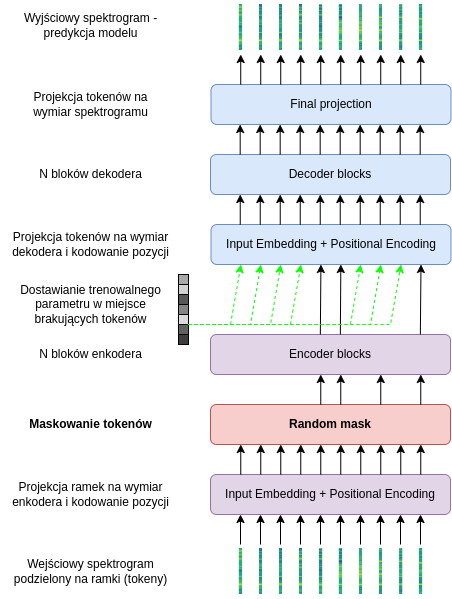
\includegraphics[width=0.8\textwidth]{./images/mae_transformer.png}
    \caption{Schemat autoenkodera uzupełniającego fragmenty spektrogramu.}
    \label{fig:mae_transformer}
\end{figure}

% opis modelu - dokładny opis na podstawie rysunku
Idąc za pomysłem twórców algorytmu MAE, zastosowana została architektura składająca się z~dwóch części --- enkodera i~dekodera --- które razem tworzą autoenkoder. Każdy z~nich jest po prostu osobnym transformerem, ale dekoder powinien być zdecydowanie mniejszy. Cały model zaprezentowany jest na rysunku \ref{fig:mae_transformer}. Na wejściu do modelu znajduje się spektrogram. Następnie, zgodnie z~opisaną już wcześniej zasadą działania transformera, ramki są rzutowane na odpowiednią dla enkodera liczbę wymiarów i~dodawane jest do nich kodowanie pozycji. Następuje później kluczowa operacja maskowania, która odbywa się na poziomie sekwencji tokenów. Polega ona na usunięciu losowej części sekwencji, zgodnie z~odpowiednimi, opisanymi poniżej założeniami. Enkoder przetwarza następnie jedynie niezamaskowane tokeny, dzięki czemu dla dużych proporcji maskowania zmniejsza się znacząco złożoność wymaganych obliczeń. Jest to jeden z~głównych atutów wspomnianego algorytmu MAE. Po przejściu przez wszystkie bloki enkodera niezamaskowana część sekwencji powinna być docelowo przedstawiana w~postaci wektorów bogatych semantycznie cech. Przed wejściem do dekodera, skrócona sekwencja jest z~powrotem rozszerzana do oryginalnej długości. Wykorzystuje się w~tym celu specjalny, ,,trenowalny'' wektor odpowiedniej długości, który jest wstawiany w~miejsce wszystkich zamaskowanych tokenów. Cała sekwencja przechodzi później przez dekoder, którego zadaniem jest wytworzyć spektrogram, jak najbardziej zbliżony do oryginalnego. Aby to zrobić, musi uzupełnić zamaskowane tokeny na podstawie informacji, jaką w~niezamaskowanej części sekwencji umieścił enkoder. Mały rozmiar dekodera wymusza wyciągnięcie jak najwięcej informacji z~widocznych tokenów przez enkoder. Co więcej, ponieważ dekoder przetwarza już pełną sekwencję tokenów, to jego rozmiar wpływa bardzo na złożoność obliczeń.

\subsection{Zasady maskowania spektrogramów}

% maskowanie spektrogramów - wstęp
Operacja maskowania spektrogramów, jak już wspomniano, odbywa się na poziomie całej sekwencji --- maskowane są zawsze całe tokeny, a~nie ich fragmenty. Jest to oczywiście jedno z~możliwych podejść, można bowiem próbować maskować również fragmenty tokenów. Zastosowane podejście pozwala jednak bardzo łatwo na optymalizację, polegającą na przetwarzaniu przez enkoder jedynie niezamaskowanej części sekwencji.

% maskowanie spektrogramów - kwestia proporcji
Indeksy wycinanych tokenów są losowane, a~proporcja między ich liczbą a liczbą pozostawionych tokenów jest hiperparametrem danego treningu samonadzorowanego. W~przypadku maskowania słów w~zdaniach \cite{devlin_bert_2019} wycinana jest jedynie niewielka część ($15\%$) sekwencji, ponieważ każdy pojedynczy token (słowo), ma już w~sobie bardzo dużo informacji --- bardzo bogate i~szerokie, abstrakcyjne znaczenie. W~przypadku maskowania obrazów \cite{he_masked_2021} jest dokładnie odwrotnie --- wycinana jest spora część obrazu ($75\%$), ponieważ pojedyncze piksele mają w~sobie niewiele informacji i~mogą być skutecznie uzupełnione przez zwykłą interpolację liniową. W~przypadku spektrogramów sytuacja jest bardziej zbliżona do obrazów, ponieważ uzupełnienie pojedynczych ramek również można zrealizować poprzez nieskomplikowaną interpolację. Co więcej, charakter spektrogramów dla utworów muzycznych jest taki, że często ich długie, trwające ułamek sekundy lub nawet kilka sekund fragmenty są stałe. Zależy to oczywiście od gatunku i~od tego, które fragmenty spektrogramu są brane pod uwagę. Jeżeli chodzi natomiast o~częstość zmian akordów w~zachodniej muzyce popularnej, to w $10$-sekundowych fragmentach będą się one często zmieniać zaledwie kilka razy. Z~tego powodu, aby zadanie uzupełniania spektrogramów było dość wymagające, maskowana część musi najprawdopodobniej zajmować przynajmniej kilkadziesiąt procent długości całej sekwencji.

% maskowanie spektrogramów - kwestia wielkości dziur
Poza proporcją maskowania, istotne jest również to, czy wycinane ramki będą tworzyły dłuższe, ciągłe fragmenty. Wynika to z~faktu, że uzupełnienie co drugiej ramki, choć proporcja maskowania wynosi $50\%$, wciąż pozostaje stosunkowo łatwym zadaniem. Natomiast uzupełnienie trwającego $2$ sekundy ciągłego fragmentu, chociaż jest to tylko piąta część całej sekwencji, stanowi zadanie znacznie trudniejsze i~wymaga głębszej interpretacji widocznych fragmentów nagrania. Dlatego też drugim hiperparametrem treningu samonadzorowanego jest liczba ciągłych bloków, na które dzielona jest cała sekwencja. Kiedy następuje operacja maskowania, tokeny są wycinane lub pozostawiane jedynie w~ciągłych grupach, tworzących te bloki. Za pomocą tego hiperparametru i~proporcji maskowania można modyfikować trudność zadania między samonadzorowanymi treningami wstępnymi.

% maskowanie spektrogramów - łatwa implementacja
Omawiając zasady maskowania spektrogramów, warto wspomnieć o~jeszcze jednej zalecie tego algorytmu --- jest on bardzo łatwy w~implementacji. Maskowanie można zrealizować jako wykonanie permutacji sekwencji tokenów i~odcięcie odpowiedniej ich liczby. Aby po przejściu przez bloki enkodera uzyskać sekwencję oryginalnej długości i~kolejności, wystarczy dokleić odpowiednią liczbę razy wektor oznaczający zamaskowane tokeny i~wykonać permutację odwrotną. Podejście to można stosować również wtedy, kiedy chce się zachować zadaną liczbę ciągłych bloków w~ramach sekwencji.

\subsection{Procedura treningu}

% eksperymenty, treningi, zbiory i~epoki
W~przypadku treningów samonadzorowanych, na pojedynczy eksperyment składa się tylko jeden trening, ponieważ nie stosowano tutaj metod takich jak walidacja krzyżowa. Sama nauka odbywa się na podstawie wszystkich danych nieoznaczonych ($10000$ utworów), które tworzą zbiór treningowy. Dane te, pomijając fakt, że nie mają oznaczeń, przetwarzane są do postaci $10$-sekundowych spektrogramów dokładnie w~taki sam sposób, jak w~treningach nadzorowanych. Stosowane są również te same augmentacje. We wszystkich wykonanych eksperymentach nienadzorowanych wykorzystany jest pełny zbiór treningowy. Mimo braku oznaczeń wciąż konieczne jest jednak aby sprawdzać, czy zbiór nie uczy się danych treningowych na pamięć. W~tym celu pierwsza z~pięciu części danych oznaczonych (same niezaugmentowane nagrania, bez oznaczeń akordów) wykorzystana jest jako zbiór walidacyjny. Dokładnie tak jak w~eksperymentach nadzorowanych, trening dzieli się na epoki, gdzie pojedyncza epoka oznacza kilkukrotnie przejście przez wszystkie nagrania treningowe, ale dla każdego z~nich losowany jest zawsze jeden $10$-sekundowy fragment.

% kroki, maskowanie, predykcja i~funkcja kosztu
Epoki dzielą się na kroki, gdzie każdy krok to równoległe przetworzenie całego \emph{batcha} $10$-sekundowych fragmentów i~jednokrotna modyfikacja parametrów modelu. W~ramach danego kroku generowana jest pojedyncza maska (lista numerów tokenów), stosowana dla wszystkich fragmentów w \emph{batchu}. Dla pojedynczej ramki wyjściowej $f' \in \mathbb{R}^F$ i~pojedynczej ramki wejściowej $f \in \mathbb{R}^F$ wyliczany jest błąd średniokwadratowy (ang. \emph{mean squared error}) odgrywający rolę funkcji kosztu, zgodnie ze wzorem:
\begin{equation}
    \textrm{MSE} = \frac{1}{F} \sum_{i=1}^{F} (f'_{i} - f_{i})^2
\end{equation}
Wartość ta jest wyliczana tylko dla tych ramek, które były zamaskowane (wycięte) i~uśredniana między nimi, oraz między sekwencjami. Ma to zmusić model do skupienia się na zadaniu rekonstrukcji, a~nie kopiowaniu wartości wejściowych.  Następnie, w~standardowy sposób, parametry całego autoenkodera są optymalizowane na podstawie gradientu błędu średniokwadratowego.  Wartość funkcji kosztu jest logowana dla każdego \emph{batcha}.

% walidacja
Po przejściu przez wszystkie przykłady treningowe z~epoki następuje etap bieżącej walidacji modelu, mający na celu uniknięcie przetrenowania. Dokładnie tak samo, jak dla danych uczących, wyliczane są predykcje na fragmentach ze zbioru walidacyjnego i~obliczana jest wartość tej samej funkcji kosztu.  Wartość ta jest logowana i~służy jedynie porównaniu z~wartością na zbiorze treningowym --- nie wylicza się na jej podstawie pochodnej i~nie optymalizuje parametrów modelu. W~przeciwieństwie do treningów nadzorowanych zbiór walidacyjny jest przetwarzany tak samo, jak zbiór treningowy, poprzez losowanie $10$-sekundowych fragmentów dla kolejnych utworów. Podejście to jest zdecydowanie wystarczające, aby ocenić, czy model zaczyna się uczyć na pamięć.

% po walidacji
Na koniec każdej epoki, stan enkodera jest zapisywany, aby umożliwić późniejsze wykorzystanie go do rozpoznawania akordów (treningów nadzorowanych). Dodatkowo, aby ułatwić ocenę stanu autoenkodera, która jest dość trudna na podstawie samej wartości błędu średniokwadratowego, wybierane są trzy losowe przykłady ze zbioru walidacyjnego. Każdy z~nich zapisywany jest w~postaci obrazka z~trzema spektrogramami: wejściowy sprzed operacji maskowania, zamaskowany przed wejściem do sieci i~predykcja sieci. Obejrzenie konkretnych predykcji modelu pozwala ocenić w~jakim stopniu rzeczywiście model nauczył się rozumieć strukturę nagrań muzycznych.

\subsection{Implementacja i~wykorzystana infrastruktura}

% implementacja i~sprzęt
Cała procedura treningu samonadzorowanego wraz z~konstrukcją autoenkodera została zaimplementowana w~pliku \url{src/training/mae_training.py}. Podobnie jak trening nadzorowany, przygotowana została możliwość treningu rozproszonego, a~wszystkie hiperparametry i~metryki są logowane do systemu \emph{MLflow}. Treningi odbywały się na jednej lub kilku kartach graficznych NVIDIA GeForce RTX 3090.

\subsection{Podsumowanie hiperparametrów treningu}

% podsumowanie hiperparametrów treningu
Wszystkie ustawienia pojedynczego treningu samonadzorowanego, włączając w~to ustawienia zbioru danych i~hiperparametry autoenkodera zostały przedstawione w~Tab. \ref{tab:mae_training_params}.  Wartości hiperparametrów z~tej tabeli są wymieniane dla każdego udokumentowanego eksperymentu. Tak samo, jak dla treningów nadzorowanych, pominięte zostały niektóre stałe lub techniczne ustawienia, opisane w~poprzednich rozdziałach. 

% wszystkie hiperparametry wynikające z~argparse (F-fixed, T-technical, X-changed between experiments)
% DATASET
% F   sample_rate=22050
% F   frame_size=2048
% F   hop_size=2048
% F   frames_per_item=100
% X   item_multiplier
% X   song_multiplier
% F   audio_preprocessing (cqt, raw)=CQT
% F   standardize_audio=YES
% X   pitch_shift_augment
% F   labels_vocabulary=MAJ_MIN
% T   subsets=None
% F   dataset_fraction=1.0
% T   use_ram_cache
% ENKODER
% X   encoder_dim
% X   encoder_n_heads
% X   encoder_n_blocks
% T   encoder_extra_features_dim=NO
% T   pretrained_encoder_path
% T   pretrained_encoder_run_name
% DEKODER
% X   decoder_dim
% X   decoder_n_heads
% X   decoder_n_blocks
% TRENING
% X   masking_ration
% X   chunks_per_item
% T   experiment_name
% T   run_name
% X   n_epochs
% X   batch_size
% X   lr
% T   ddp

\begin{table}
    \centering
    \caption{Hiperparametry pojedynczego samonadzorowanego treningu wstępnego.}
    \label{tab:mae_training_params}
    \begin{tabular}{|l|p{0.6\linewidth}|}
        \hline \multicolumn{2}{|c|}{ZBIÓR DANYCH} \\ \hline
        \code{item\_mutliplier} & Liczba przykładów zwracanych dla jednego utworu \\
        \code{song\_multiplier} & Liczba przejść przez wszystkie utwory w~jednej epoce \\
        \code{augment} & Czy zastosowano augmentacje \\
        \hline \multicolumn{2}{|c|}{ENKODER} \\ \hline
        \code{encoder\_dim} & Liczba wymiarów pojedynczego tokena przechodzącego przez enkoder \\
        \code{encoder\_n\_heads} & Liczba równoległych operacji MSA w~enkoderze\\
        \code{encoder\_n\_blocks} & Liczba bloków w~enkoderze \\
        \hline \multicolumn{2}{|c|}{DEKODER} \\ \hline
        \code{decoder\_dim} & Liczba wymiarów pojedynczego tokena przechodzącego przez dekoder \\
        \code{decoder\_n\_heads} & Liczba równoległych operacji MSA w~dekoderze\\
        \code{decoder\_n\_blocks} & Liczba bloków w~dekoderze \\
        \hline \multicolumn{2}{|c|}{TRENING} \\ \hline
        \code{masking\_ratio} & Proporcja maskowania --- jaka część sekwencji tokenów jest wycinana \\
        \code{chunks\_per\_item} & Liczba ciągłych, niepodzielnych bloków w~sekwencji \\
        \code{n\_epochs} & Liczba epok w~treningu \\
        \code{batch\_size} & Liczba utworów przetwarzanych w~jednym kroku \\
        \code{lr} & Współczynnik uczenia \\ \hline
    \end{tabular}
\end{table}

\chapter{Rozpoznawanie akordów muzycznych}

% wstęp/skrót całego rozdziału
Rozpoznawanie akordów muzycznych zostało zrealizowane za pomocą sieci neuronowych. Wykorzystana
została popularna ostatnio w wielu obszarach architektura transformera
\cite{vaswani_attention_2017}. Modele tego typu były wykorzystywane w najnowszych pracach związanych
z rozpoznawaniem akordów, w tym w pracy stanowiącej główny punkt odniesienie dla niniejszych badań
\cite{park_bi-directional_2019}.

Podczas realizacji zadania rozpoznawania akordów, w pierwszej kolejności zreprodukowane zostały
wyniki z pracy referencyjnej. W tym celu wykonany został zwykły trening nadzorowany, z
wykorzystaniem zbliżonego zbioru danych, zbliżonej procedury i identycznego modelu, jak w
oryginalnych badaniach.

W następnej kolejności model został uproszczony i pozbawiony autorskich usprawnień, po czym wykonana
została seria eksperymentów mająca na celu uzyskać tym modelem jak najlepsze wyniki. Celem tego
etapu było przygotowanie punktu odniesienia dla późniejszych eksperymentów z uczeniem
nienadzorowanym. Model został uproszczony aby nie zaciemniać właściwego tematu pracy, jakim jest
wykorzystanie uczenia nienadzorowanego.

Mając przygotowany działający i stosunkowo prosty model, który uzyskuje wyniki zbliżone do
najlepszych w literaturze, można było przejść do treningów nienadzorowanych, a dokładnie
samonadzorowanych (ang. \emph{self-supervised}). Wykonana została seria czasochłonnych i
zasobożernych eksperymentów, wykorzystujących jedynie dane bez oznaczeń, dzięki którym uzyskano
pretrenowane (ang. \emph{pre-trained}) sieci. Na końcu te pretrenowane modele zostały dotrenowane do
zadania rozpoznawania akordów i wyniki porównano z tymi, uzyskanymi bez uczenia wstępnego.

% co zawiera rozdział
W niniejszym rozdziale opisana została szczegółowo wykorzystana architektura sieci neuronowej.
Następnie przedstawione zostały procedury i zasady treningów nadzorowanego i nienadzorowanego oraz
reguły oceny wytrenowanego modelu. Na końcu opisane zostały wszystkie wykonane eksperymenty i
przeprowadzona została dyskusja otrzymanych wyników.

% model (model.py), trening nadzorowany (training.py), trening nienadzorowany (mae_training.py) i
% ewaluacja (evaluate.py)
\section{Algorytm rozpoznawania akordów muzycznych}

% wstęp - dyskusja na temat podejścia do rozpoznawania akordów (TODO: czy to dobry wstęp i w ogóle
% dobry tytuł tej pierwszej z dwóch części rozdziału, może ta dyskusja powinna być gdzieś indziej)
Jak wspomniano powyżej, do rozpoznawania akordów muzycznych wykorzystano sieci neuronowe. Modele te
są jednak bardzo ogólne i wykorzystując je, wciąż można podejść do zadania rozpoznawania akordów na
bardzo wiele różnych sposobów. Samo zadanie polega właściwie na podzieleniu wejściowego nagrania
muzycznego na logiczne części, w których wybrzmiewają pojedyncze, rozpoznane przez algorytm akordy.
Można więc potraktować to zadanie jako dwa podzadania, albo przeformułować je tak, aby było prostsze
ale dawało takie same rezultaty. 

Po pierwsze należy więc zadać sobie pytanie, z jaką dokładnością mają być rozpoznawane chwile
rozpoczęcia i zakończenia trwania akordów. Sygnał dźwiękowy jest sygnałem ciągłym, ale zapisany jest
w postaci cyfrowej z określoną częstotliwością próbkowania. Można zatem próbować rozpoznawać akordy
z największą możliwą dokładnością, czyli co do pojedynczej próbki. Jest to jednak dokładność
zdecydowanie nadmiarowa w kontekście tego zadania. Zakładając z kolei, że dane wejściowe nie
będą miały postaci surowych próbek ale postać spektrogramu, dokładność rozpoznawania można
ograniczyć do pojedynczych ramek czasowych tworzących spektrogram. Podejście takie jest o tyle
proste, że zadanie rozpoznawania akordów staje się stricte zadaniem klasyfikacji ramek spektrogramu,
które są po prostu wektorami pewnych cech. Uzyskana dokładność czasowa, rzędu dziesiątych części
sekundy, wydaje się być jak najbardziej wystarczająca. Takie też podejście zostało zastosowane w
niniejszej pracy, co jasno widać po opisanym w poprzednim rozdziale wstępnym przetwarzaniu danych.

Kolejnym tematem jest sposób przetwarzania ramek spektrogram przez sieć neuronową. Teoretycznie
każda ramka może być najpierw klasyfikowana osobno, bez uwzględnienia kontekstu przed i po danej
chwili czasu. Powstała w ten sposób, zapewne dość zaszumiona sekwencja akordów, może być wygładzona
kolejnym algorytmem. Wiele podejść tego typu było wcześniej stosowanych. Lepszym pomysłem wydaje się
jednak wykorzystanie szerszego kontekstu czasowego na etapie rozpoznawania pojedynczych akordów.
Można np.  podawać na wejście sieci dłuższy (trwający więcej niż sekundę) fragment a rozpoznawać
jedynie akord brzmiący na samym środku tego fragmentu, jak to zostało zrobione w
\cite{korzeniowski_fully_2016}.  Wciąż można później zaaplikować algorytm uwzględniający szerszy
kontekst, czyli np. konkretne progresje akordów. Najlepiej by jednak było, gdyby model rozpoznający
akordy był jeden i łączył w sobie zarówno informacje lokalne (brzmiące w danym ułamu sekndy
częstotliwości) jak i informacje globalne (progresje akordów). Można więc podawać na wejście sieci
od razu dłuższy fragment utworu i z dokładnością do ramek czasowych dokonywać swego rodzaju
segmentacji semantycznej, czyli przypisywać klasę dla każdej ramki. Takie podejście zostało właśnie
zastosowane w \cite{park_bi-directional_2019}. Idąc za tym najprostszym i być może najbardziej
naturalnym pomysłem zastosowano go również w niniejszej pracy. 

\subsection{Opis wykorzystanego modelu sieci neuronowej}

Do rozpoznawani akordów, podobnie jak w \cite{park_bi-directional_2019}, wykorzystany został
popularny w ostatnim latach model sieci neuronowej o nazwie \emph{Transformer}. W niniejszej pracy,
poza fazą reprodukcją wyników z \cite{park_bi-directional_2019}, wykorzystana została jak
najprostsza i jak najbardziej zbliżona do oryginału wersja tego modelu. Implementacja została,
przygotowana samodzielnie (plik \url{src/training/model.py}) na bazie literatury i innych
implementacji.

\subsubsection{Krótka historia transformerów}

% krótka historia transformera (TODO: czy to do przeglądu literatury czy tutaj)
Model transformera został oryginalnie wprowadzony jako model do przetwarzania języka naturalnego, w
pracy \cite{vaswani_attention_2017}. Była to architektura typu \emph{enkoder-dekoder}, służąca np.
do tłumacznie z jednego języka na drugi. Wcześniej do zadań związanych z językiem naturalnym były
głównie wykorzystywane sieci rekurencyjne, które miały problem, aby dobrze radzić sobie z długimi
sekwencjami słów --- zapominały kontekst jeżeli przetwarzany tekst nie był dość krótki. W celu
rozwiązania tego problemu wprowadzono mechanizm atencji (ang. \emph{attention}), który pozwalał
uwzględnić dalszy kontekst zdania \cite{bahdanau_neural_2016}. Pomysł twórców transformera polega na
tym, aby zrezygnować z sieci rekurencyjnych i pozostawić jedynie mechanizm atencji, w połączeniu z
warstwami liniowymi i funkcjami aktywacji (MLP). Transformer nie jest więc ani siecią rekurencyjną,
ani siecią splotową. Po odniesieniu ogromnego sukcesu w NLP (dziś praktycznie wszystkie modele do
NLP są budowane na bazie transformerów), architektura ta została wykorzystana również w
przetwarzaniu obrazów \cite{dosovitskiy_image_2021}. Na potrzeby klasyfikacji zdjęć została nieco
uproszczona ponieważ pozostawiony został sam enkoder. Na tym polu transformery również odniosły
sukces, chociaż nie wyparły sieci splotowych \cite{liu_convnet_2022}, tak jak wyparły sieci
rekurencyjne. Ostatecznie modele tego typu zostały wykorzystane również do przetwarzania dźwięku, w
tym do klasyfikacji dźwięków \cite{gong_ast_2021} i do rozpoznawania mowy
\cite{kim_squeezeformer_2022}. Transformery są więc dziś bardzo popularnymi modelami, które znajdują
zastosowanie praktycznie w każdej dziedzinie wykorzystującej uczenie maszynowe.

\subsubsection{Ogólny opis architektury}

\begin{figure}
    \centering
    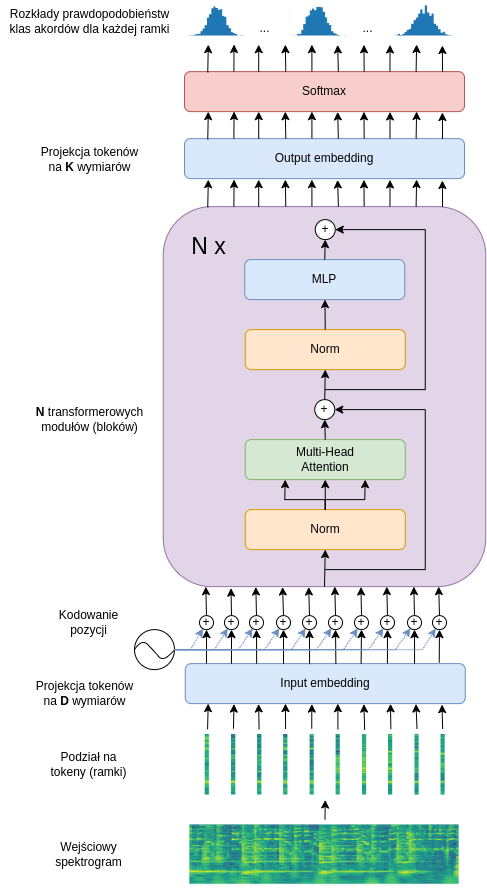
\includegraphics[width=0.8\textwidth]{./images/transformer.png}
    \caption{Schemat modelu transformera do rozpoznawania akordów muzycznych}
    \label{fig:transformer}
\end{figure}

% ogólny opis architektury - wejście
Rysunek \ref{fig:transformer} prezentuje wykorzystany do treningów model sieci neuronowej ---
transformer. Architektura tego modelu jest bardzo prosta. Na wejście sieci podawany jest składający
się z $N$ ramek spektrogram $\defmatrix{S}{N}{F}$, który następnie dzielony jest (tylko ideowo, w
praktyce to wciąż pojedyncza macierz) na ramki (wektory $\vec s_i \in \mathbb{R}^F$). Ramki pełnią
rolę tokenów, czyli np. kolejnych słów w przypadku przetwarzania języka naturalnego. Transformer
przetwarza cały ciąg tokenów równolegle, co jest jego podstawową przewagą nad sieciami
rekurencyjnymi, które przetwarzają ciąg tokenów w sposób sekwencyjny. W praktyce jednocześnie przez
sieć może przejść kilka ciągów tokenów, czyli cały \emph{batch} sekwencji. Długość sekwencji tokenów
jest zupełnie arbitralna, ten sam model może przetwarzać sekwencje różnej długości, zarówno w
treningu jak i później, podczas inferencji.

% ogólny opis architektury - input embedding i positional encodding
W pierwszej kolejności sekwencja ramek (macierz $\matrix{S}$) przechodzi przez pojedynczą warstwę
liniową, która rzutuje tokeny wejściowe na wybraną dla danego modelu liczbę wymiarów
$d_{\mathrm{model}}$:
\begin{equation}
    \matrix{T_{in}} = \matrix{S} \matrix{W_{in}}
\end{equation}
gdzie $\defmatrix{T_{in}}{N}{d_{\mathrm{model}}}$ to wyjściowa macierz tokenów a
$\defmatrix{W_{in}}{F}{d_{\mathrm{model}}}$ to macierz parametrów tej warstwy. Liczba wymiarów
$d_{\mathrm{model}}$, podobnie jak liczba tokenów $N$, nie zmienia się podczas przechodzenia przez
kolejne warstwy, co różni transformer od sieci splotowych, gdzie rozmiar danych przechodzących przez
sieć jest sukcesywnie zmniejszany. W rzeczywistości istnieją architektury oparte o oryginalny
transformer, które podobnie jak sieć splotowa, zmniejszają rozmiar danych wejściowych
\cite{liu_swin_2021}, ale to tylko głupie wymysły Microsoftu. Przed wejściem do stanowiących
właściwą część transformera serii bloków, do tokenów dokładana jest informacja o ich pozycji w
sekwencji --- jest to kodowanie pozycji (ang. \emph{positional encoding}). Szczegóły tej operacji
zostały opisane poniżej.

% ogólny opis architektury - bloki, w tym MLP i normalizacja
Centralną część transformera stanowi ciąg identycznych bloków BLK. Liczba tych bloków ($B$), w
połączeniu z wymiarowością tokenów ($d_{\mathrm{model}}$), stanowią główne hiperparametry modelu i
decydują o jego rozmiarze. Każdy blok składa się z dwóch głównych warstw: warstwy atencyjnej MSA
(ang. \emph{Mulit-Head Self-Attention}) i niewielkiego perceptrona wielowarstwowego MLP (ang.
\emph{Mulitlayer Perceptron}). Każdą z tych warstw poprzedza normalizacja Norm typu \emph{Layer
Normalization} \cite{ba_layer_2016}, a kończy połączenie rezydualne \cite{he_deep_2015}, czyli
dodanie do wartości na wyjściu nieznormalizowanej wartości z wejścia. Operacje realizowane przez
pojedynczy blok dla ciągu tokenów $\defmatrix{T}{N}{d_{\mathrm{model}}}$ można opisać równaniami:
\begin{eqnarray}
     \textrm{MSA}'(\matrix{T}) = \textrm{MSA}(\textrm{Norm}(\matrix{T})) + \matrix{T} \\
     \textrm{MLP}'(\matrix{T}) = \textrm{MLP}(\textrm{Norm}(\matrix{T})) + \matrix{T} \\
     \textrm{BLK}(\matrix{T}) = \textrm{MLP}'(\textrm{MSA}'(\matrix{T}))
\end{eqnarray}
Zastosowana nomalizacja aplikowana jest niezależnie (choć równolegle) dla każdego tokena $t \in
\mathbb{R}^{d_{\mathrm{model}}}$ z sekwencji $\matrix{T}$. Polega ona na odjęciu wartości średniej
tokena oraz podzieleniu przez jego odchylenie standardowe. Przedstawia to wzór:
\begin{equation}
    \textrm{Norm}(t) = \frac{t - \textrm{E}[t]}{\sqrt \textrm{Var}[t]} \cdot \gamma + \beta
\end{equation}
gdzie $\gamma$ i $\beta$ to trenowane parametry warstwy, przesuwające i skalujące odpowiednio wynik
normalizacji. Jeżeli chodzi o perceptron wielowarstwowy, to ma ona zawsze dwie warstwy ukryte, z
wymiarem ukrytym czterokrotnie większym niż $d_{\mathrm{model}}$ oraz funkcją aktywacji GELU.
\begin{equation}
    \textrm{MLP}(\matrix{T}) = \textrm{GELU}(\matrix{T}\matrix{W_1} + b_1)\matrix{W_2} + b_2
\end{equation}
gdzie wejściem jest sekwencja tokenów $\defmatrix{T}{N}{d_{\mathrm{model}}}$, macierze
$\defmatrix{W_1}{d_{\mathrm{model}}}{4d_{\mathrm{model}}}$,
$\defmatrix{W_2}{4d_{\mathrm{model}}}{d_{\mathrm{model}}}$ oraz wektory (dodawane do każdego wiersza
odpowiedniej macierzy) $b_1 \in \mathbb{R}^{4d_{\mathrm{model}}}$ i $b_2 \in
\mathbb{R}^{d_{\mathrm{model}}}$ to parametry dwóch warstw ukrytych perceptrona wielowarstwowego.

% ogólny opis architetury - dropout
W rzeczywistości pojedynczy blok zawiera jeszcze jeden opcjonalny element, jakim są warstwy
\emph{dropout}, umieszczone po każdym z dwóch połączeń rezydualnych, czyli w połowie bloku i na jego
wyjściu. Dodatkowo \emph{dropout} może być stosowany również przed wejściem do sieci, czyli
bezpośrednio na spektrogramie. Warstwy tego typu zerują z wybranym prawdopodobieństwem niektóre z
przechodzących przez nie wartości w celu regularyzacji sieci i uniknięcia przetrenowania. Technika
ta jest opcjonalna i nie była stosowana we wszystkich eksperymentach.

% ogólny opis architektury - wyjście (klasyfikacja)
Po serii bloków następuje ostatnia część modelu, odpowiedzialna za klasyfikację. Najpierw,
utrzymywana przez wszystkie bloki, wymiarowość tokenów jest zmieniana przez warstwę liniową, w
zależności od liczby klas $K$.
\begin{equation}
    \matrix{T_{out}} = \matrix{T} \matrix{W_{out}}
\end{equation}
gdzie $\defmatrix{T_{out}}{N}{K}$ to macierz wyjściowa, $\defmatrix{T}{N}{d_{\mathrm{model}}}$ to
macierz sekwencji tokenów a $\defmatrix{W_{out}}{d_{\mathrm{model}}}{K}$ to macierz parametrów tej
warstwy liniowej. Następnie dla każdego tokena $t \in \mathbb{R}^K$ zwracany jest rozkład
prawdopodobieństwa przynależności do poszczególnych klas akordów, za pomocą funkcji \emph{softmax}:
\begin{equation}
    \textrm{softmax}(t_i) = \frac{\exp{t_i}}{\sum_{j=1}^{K}\exp{t_j}}
\end{equation}
gdzie $t_i$ to $i$-ty element wektora (tokena) $t$. Podsumowując, na wejściu sieci jest spektrogram,
składający się z $N$ ramek i $F$ cech, a na wyjściu jest $N$ rozkładów prawdopodobieństwa między $K$
klas, dla każdej z ramek spektrogramu. Wszystkie ramki spektrogramu są więc klasyfikowane
jednocześnie, ale z uwzględnieniem kontekstu, jaki tworzą razem.

\subsubsection{Kodowanie pozycji tokenów}

% positional encoding
Jak widać na rysunku \ref{fig:transformer}, pomiędzy projekcją tokenów wejściowych a wejściem do
serii bloków, jest jeszcze etap kodowania pozycji każdego z tokenów. Etap ten jest niezbędny aby
zawrzeć w każdym z tokenów informację o tym, jaka jest jego pozycja w sekwencji. W przypadku sieci
rekurencyjnych, informacja ta jest zawarta niejawnie, poprzez przetwarzanie tokenów jeden po drugim,
w odpowiedniej kolejności. W przypadku transformerów, gdzie tokeny są przetwarzane równolegle,
informacja ta musi być dodana jawnie.  Istnieje wiele sposobów, według których można zakodować
pozycję tokenów, głównie dzielących się na wykorzystanie wartości wyuczonych (parametry modelu) i
stałych (odpowiednia funkcja).  W niniejszej pracy wykorzystane zostało podejście oryginalnych
twórców transformera, oparte o wartości funkcji sinus i kosinus. Polega ono na tym, że dla każdego
tokena (dla każdej pozycji) generuje się wektor, który ma tę samą liczbę wymiarów co token, dzięki
czemu może być do niego dodany. Wartości tych wektorów zdefinowane są wzorami:
\begin{equation}
    PE_{(\textrm{pos},2i)} = \sin(\textrm{pos}/10000^{2i/d_{\textrm{\tiny model}}})
\end{equation}
\begin{equation}
PE_{(\textrm{pos},2i + 1)} = \cos(\textrm{pos}/10000^{2i/d_{\textrm{\tiny model}}})
\end{equation}
Równania te oznaczają, że każdy wymiar wektora kodującego pozycję odpowiada sinusoidzie o innej
częstotliwości. Parzyste pozycje w wektorze to wartości odpowiednich funkcji sinus dla danej
pozycji, a nieparzyste to wartości funkcji kosinus dla danej pozycji. Stosowany jest również
wariant, gdzie pierwsza połowa wektora to wartości funkcji sinus a druga to wartości funkcji
kosinus. Autorzy uzasadniają, że użycie tych funkcji pozwala modelowi łatwo wykorzystywać informację
o pozycji, ponieważ między wektorami prezentującymi różne pozycje występują zależności liniowe. Na
rysunku \ref{fig:positional_encoding} przedstawiono graficzną reprezentację wektorów kodujących
pozycję, dla sekwencji składającej się ze 100 tokenów (wiersze), gdzie liczba wymiarów każdego z
nich to 256 (kolumny).
\begin{figure}
    \centering
    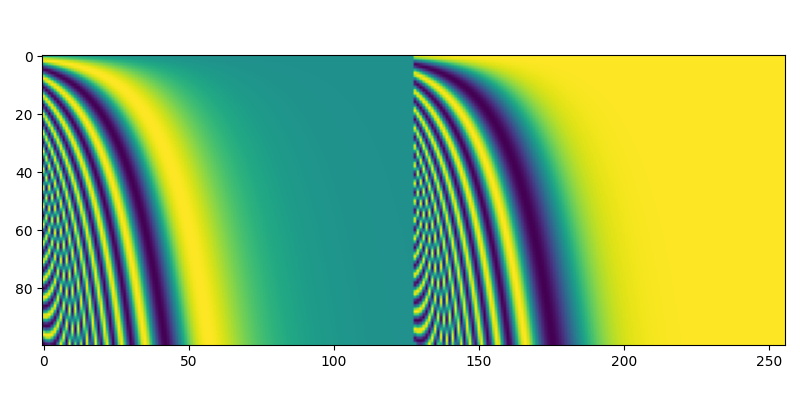
\includegraphics[width=1.0\textwidth]{./images/positional_encoding.png}
    \caption{Przykład wektorów kodujących pozycję dla sekwencji 100 tokenów o wymiarowości 256}
    \label{fig:positional_encoding}
\end{figure}

\subsubsection{Multi-Head Self-Attention}

% mutli-head self-attention - wstęp
Najważniejszą część transformera stanowi warstwa atencyjna MSA. Jako jedyna w całym modelu
odpowiada ona za ,,wymianę'' informacji między tokenami --- uwzględnienie kontekstu pozostałych
tokenów w sekwencji, podczas tworzenia nowej reprezentacji danego tokena.

% mutli-head self-attention - ogólnie o mechaniźmie attention
Sama idea mechanizmu \emph{Attention} polega na tym, że mając dla danego tokena wejściowego
zapytanie (ang. \emph{query}) i mając zbiór par klucz-wartość (ang. \emph{key-value}) związanych z
innym (lub tym samym) ciągiem tokenów, wylicza się nową reprezentację tokena jako ważoną sumę tych
wartości, gdzie wagi są wyliczane na podstawie dopasowania zapytania do kluczy. Wagi te informują
więc o tym, jak dużo uwagi powinno poświęcić się danej wartości, tworząc nową reprezentację danego
tokena. W przypadku zadania tłumaczenia maszynowego, mechanizm ten pozwala skupić się na
odpowiednich częściach sekwencji wejściowej, podczas tworzenia sekwencji wyjściowej. Jeżeli zarówno
zapytania jak i pary klucz-wartość pochodzą z tej samej sekwencji tokenów, mamy do czynienia z
\emph{Self-Attention}. Warstwa tego typu wyznacza więc dla każdego tokena w sekwencji zapytanie,
klucz i wartość, a następnie tworzy jego nową reprezentację jako ważoną sumę wartości pozostałych
tokenów. Informacje zakodowane w poszczególnych tokenach mieszają się zatem między sobą. W praktyce
warstwa atencyjna w transformerze realizuje równolegle kilka niezależnych operacji
\emph{Self-Attention}, których wyniki na końcu są łączone w całość, stąd też nazwa \emph{Multi-Head
Self-Attention}. Pozwala to uzyskać lepsze rezultaty niż pojedyncza operacja, nawet jeżeli
wykorzysta się niżej wymiarowe reprezentacje.

% mutli-head self-attention - dokładnie jak działa, wzorki
Na wejściu warstwy atencyjnej w transformerze znajduje się macierz
$\defmatrix{T}{N}{d_{\mathrm{model}}}$, czyli sekwencja $N$ tokenów. Dla każdego z nich, za pomocą
zwykłych warstw liniowych, wylicza się $H$-krotnie trzy wektory: zapytanie $q_i \in
\mathbb{R}^{d_k}$, klucz $k_i \in \mathbb{R}^{d_k}$ oraz wartość $v_i \in \mathbb{R}^{d_v}$, gdzie
$i \in [1, H]$. Dla całej sekwencji tokenów wektory te tworzą macierze $\defmatrix{Q_i}{N}{d_k}$,
$\defmatrix{K_i}{N}{d_k}$ oraz $\defmatrix{V_i}{N}{d_v}$. Przedstawiają to równania:
\begin{eqnarray}
    \matrix{Q_i} = \matrix{T} \matrix{W_i^Q} \\\
    \matrix{K_i} = \matrix{T} \matrix{W_i^K} \\\
    \matrix{V_i} = \matrix{T} \matrix{W_i^V} \\\
\end{eqnarray}
gdzie macierze $\defmatrix{W_i^Q}{d_{\mathrm{model}}}{d_k}$,
$\defmatrix{W_i^K}{d_{\mathrm{model}}}{d_k}$ oraz $\defmatrix{W_i^V}{d_{\mathrm{model}}}{d_v}$ to
macierze parametrów warstw liniowych tworzących $i$-tą trójkę: zapytanie, klucz i wartość.

Dla pojedynczej trójki macierzy $\matrix{Q}$, $\matrix{K}$ i $\matrix{V}$, operacja
\emph{Self-Attention} wygląda następująco:
\begin{equation} \label{eq:sa}
    \textrm{SA}(\matrix{Q}, \matrix{K}, \matrix{V}) = \textrm{softmax}(\frac{\matrix{Q}\matrix{K^T}}{\sqrt{d_k}})\matrix{V}
\end{equation}
Człon ,,$\textrm{softmax}(\frac{\matrix{Q}\matrix{K^T}}{\sqrt{d_k}})$'' oznacza wyliczenie macierzy
atencji między wszystkimi parami klucz-zapytanie, poprzez wykonanie iloczynów skalarnych dla
każdej z tych par, przeskalowanie uzyskanych wartości i wykorzystanie normalizującej funkcji
\emph{softmax}. Dlatego też funkcja SA nazywa się właściwie \emph{Scaled Dot-Product Attention}.
Wartości w uzyskanej macierzy atencji pełnią rolę wag, które następnie są użyte do stworzenia
nowej reprezentacji wszystkich tokenów, za pomocą średniej ważonej wektorów z macierzy $\matrix{V}$.
Wynik operacji SA jest więc macierzą, o wymiarach $N \times d_v$.

Cała opracja \emph{Multi-Head Self-Attention} polega na $H$-krotnym wykonaniu operacji
\emph{Self-Attention}, których wektory wynikowe są łączone i ostatecznie rzutowane z powrotem na
$d_{\mathrm{model}}$ wymiarów. Przedstawiają to poniższe wzory:
\begin{equation}
    \textrm{MSA}(\matrix{T}) = \textrm{Concat}(\textrm{SA}(\matrix{Q_1}, \matrix{K_1}, \matrix{V_1}), ..., \textrm{SA}(\matrix{Q_H},
    \matrix{K_H}, \matrix{V_H}))\matrix{W^O}
\end{equation}
gdzie macierz $\defmatrix{W^O}{Hd_v}{d_{\mathrm{model}}}$ to parametry ostatniej w ramach bloku
atencyjnego warstwy liniowej, która rzutuje sklejone wektory z pojedynczych operacji SA na
początkowe $d_{\mathrm{model}}$ wymiarów. Dzięki temu wymiarowość tokenów na wyjściu z warstwy
atencyjnej pozostaje taka sama jak na wejściu. W niniejszej pracy zastosowane zostało powszechne
podejście, aby liczba wymiarów wektorów zapytań, kluczy i wartości ustalić z góry i uzależnić od
liczby wymiarów tokenów i liczby równoległych operacji SA. Zależność ta jest następująca:
\begin{equation}
    d_k = d_v = \frac{d_{\mathrm{model}}}{H}
\end{equation}
Poza wspomnianymi wcześniej hiperparametrami $B$ i $d_{\mathrm{model}}$ istotna dla funkcjonowania
modelu jest również liczba $H$ równoległych operacji SA, nazywana również ,,liczbą głów''. Wszystkie
hiperparametry transformera zostały zebrane w tabeli \ref{tab:transformer_params}.

\begin{table}
    \centering
    \caption{Hiperparametry transformera}
    \label{tab:transformer_params}
    \begin{tabular}{|c|l|} \hline
        Symbol & Znaczenie \\ \hline
        $F$ & Wymiarowość na wejściu \\
        $d_{\mathrm{model}}$ & Wymiarowość tokenów wewnątrz sieci \\
        $B$ & Liczba bloków transformera \\
        $H$ & Liczba ,,głów'' w bloku MSA \\
        $K$ & Liczba klas na wyjściu \\
        $p_d$ & Prawdopodobieństwo warstw \emph{dropout} \\ \hline
    \end{tabular}
\end{table}

\subsubsection{Dwukierunkowy transformer do rozpoznawania akordów --- BTC}

W pracy referencyjnej \cite{park_bi-directional_2019} autorzy postanowili wprowadzić drobne
modyfikacje w stosunku do oryginalnego bloku transformera tworząc swój autorski model nazwany
\emph{bi-directional transformer for chord recognition} (BTC). Pierwszą z nich jest zamiana warstw
liniowych w module MLP, na jednowymiarowe warstwy splotowe z polem recepcyjnym szerokości 3 tokenów.
Według autorów ma to ułatwić sieci tworzenie bardziej ,,wygładzonych'' predykcji i lepsze
wykorzystanie kontekstu otaczającego każdą ramkę. Druga różnica polega na tym, że pojedynczy blok
transformerowy został rozbity na dwa, które dostają te same wartości na wejściu, a ich wartości
wyjściowe są łączone za pomocą dodatkowej warstwy liniowej. Bloki te różnią się operacją MSA.
Została w nich zastosowana technika maskowania, polegająca na modyfikacji macierzy atencji (wzór
\ref{eq:sa}) w ten sposób, że dla danego tokena, wagi wszystkich wcześniejszych lub późniejszych
tokenów są zerowane. Oznacza to, że tworząc nową reprezentację danego tokena wykorzystuje
się jedynie tokeny poprzedzające, lub następujące po nim. W modelu BTC, każdy z dwóch bloków
tworzących moduł MSA ma inny kierunek maskowania. Technika ta ma zmusić model do pełnego
wykorzystywania zarówno wcześniejszego jak i późniejszego kontekstu przy klasyfikacji danej ramki.

\subsection{Procedura treningu nadzorowanego}
TODO

\subsection{Procedura samonadzorowanego treningu wstępnego}
TODO

\subsection{Zasady ewluacji modelu}
TODO


\section{Eksperymenty}
TODO

\chapter{Podsumowanie} \label{chapter:summary}

W ramach niniejszej pracy przeprowadzone zostały badania na temat zastosowania nienadzorowanego uczenia sieci neuronowych w zadaniu rozpoznawania akordów muzycznych. Przeanalizowana została odpowiednia literatura i wyszukane zostały dostępne zbiory danych oznaczonych. Następnie przygotowana została metoda automatycznego gromadzenia nagrań z ogólnodostępnych źródeł. Po zgromadzeniu danych zaprojektowana została adaptacja nienadzorowanego algorytmu uczenia sieci neuronowej na nagraniach muzycznych. Zaimplementowane zostały niezbędne skrypty, pozwalające przeprowadzać dwa rodzaje treningów sieci o architekturze transformera. Wykonane zostały wreszcie serie eksperymentów, weryfikujących skuteczność zaproponowanego podejścia.

% lipne dane
Pierwszy wniosek z przeprowadzonych badań dotyczy zastosowanego, automatycznego sposobu gromadzeni danych. Zasadniczo metoda ta nie sprawdziła się zbyt dobrze i doprowadziła do niższej niż w literaturze jakości klasyfikacji akordów. Zgromadzone badania nie są wystarczająco dobrze dopasowane do znalezionych oznaczeń i uniemożliwiają skuteczny trening modelu oraz jego rzetelną ewaluację. Właściwie to nierzetelna ewaluacja jest głównym problemem, ponieważ znane są przykłady prac, kiedy model jest trenowany na zaszumionych danych. Aby jednak móc ocenić jego jakość i porównać z innymi wynikami w literaturze, konieczny jest chociaż stosunkowo niewielki, niezaszumiony zbiór. Zbiór taki nie został jednak przygotowany w ramach niniejszej pracy, co uniemożliwia dobre porównanie z badaniami innych autorów. Właściwym tematem pracy są jednak metody nienadzorowane i korzyści z nich pochodzące. Zaszumiony zbiór nie uniemożliwia dokładnego zbadania tego tematu.

% udane treningi nienadzorowane
Jeżeli chodzi o przeprowadzone treningi nienadzorowane, to zakończyły się one sukcesem. Udało się wykazać, że model skutecznie uczył się uzupełniać zamaskowane fragmenty spektrogramów. Pozostaje kwestią sporną, czy wykonanie tego zadania wymagało ekstrakcji bardzo abstrakcyjnych i wysokopoziomowych cech. Faktem jest, że dotrenowanie pretrenowanych w sposób samonadzorowany enkoderów na zadaniu rozpoznawania akordów prowadziło do nieznacznej poprawy wyników i zdecydowanie krótszego czasu treningu.

% zysk czasowy
Osiągnięty zysk w czasie treningu należy uznać za sukces. Kilkukrotne skrócenie czasu treningu przekłada się na realnie mniejsze koszty wytwarzania modeli, które mogą być używane w różnego rodzaju aplikacjach. Możliwie jest również dzięki temu wykonywanie większej liczby treningów w krótszym czasie i w związku z tym, przeprowadzanie dokładniejszych, rzetelniejszych badań. Co więcej, pretrenowany model ma charakter ogólny i tak naprawdę powinien przynieść podobną korzyść, kiedy byłby dotrenowywany na innych zadaniach niż rozpoznawanie akordów, takich jak rozpoznawanie gatunku muzycznego, instrumentów czy ekstrakcja linii melodycznej.

% zysk dokładności - probem leży gdzie indziej
Niewielki zysk w dokładności rozpoznawania akordów można interpretować na wiele sposobów. Najprawdopodobniej jest on jednak związany z tym, że zadanie rozpoznawania akordów jest zadaniem stosunkowo prostym dla modelu sieci neuronowej. Jakość wyników zależy natomiast głównie od danych uczących, które w tym przypadku były bardzo zaszumione. Chcąc osiągnąć lepsze wyniki na tym zadaniu, należałoby przede wszystkim skupić się na poprawieniu danych. Metody nienadzorowane są być może w tym przypadku nadmiarowe, choć jak się okazuje i tak prowadzą do poprawy wyników. Widać to szczególnie kiedy danych uczących jest skrajnie mało, wtedy trening wstępny pozwala znacząco poprawić jakość klasyfikacji.

% perspektywy
Perspektywy dalszych badań są bardzo różne. Jeżeli chcieć skupić się konkretnie na zadaniu rozpoznawania akordów, to wobec przeprowadzonych eksperymentów i poczynionych obserwacji, słuszniejszym wydaje się zrezygnować z tak złożonych i wymagających metod, jak treningi nienadzorowane. Należałoby natomiast szukać szczegółowych przyczyn niemożności osiągnięcia lepszych wyników, zwłaszcza w kontekście jakości danych uczących i walidacyjnych. Z drugiej zaś strony, w niniejszej pracy wykazano korzyści i duży potencjał metod nienadzorowanych w obszarze MIR. Aby kontynuować badania na ten temat, należałoby przede wszystkim wykonać znacznie więcej eksperymentów nienadzorowanych i wykorzystać pretrenowane modele w innych zadaniach, nie tylko w rozpoznawaniu akordów. Jeżeli wykorzystać przy tym nawet niewielkie, ale jakościowo dobre zbiory danych, możliwe byłoby znalezienie optymalnego sposobu przeprowadzania treningu samonadzorowanego. Trzeba również pamiętać, że istnieją jeszcze inne algorytmy, które są możliwe do wykorzystania i mogą dawać lepsze rezultaty niż zastosowane podejście, oparte o metodę MAE.


\printbibliography

\listoffigures
\listoftables

\end{document}
